 %\documentclass[12pt]{dalthesis}
\documentclass[12pt]{book}
 %  \documentclass [12pt , letterpaper , twoside , openright ]{book}


%\documentclass[a4paper,11pt]{article}
\usepackage[utf8]{inputenc}
\usepackage{graphicx}


\usepackage{helvet}
\usepackage{graphicx,makeidx,multicol}
\usepackage{amsmath,amsthm,latexsym,amssymb}
\usepackage{float}
\usepackage{epsfig, graphicx,xspace,color,graphics}
\usepackage{xspace}
\usepackage{setspace}
\usepackage{array,ragged2e}

\usepackage{cite}
\usepackage{natbib}
\usepackage{amsfonts}
\usepackage{amsmath}
\usepackage{mathtools}
\usepackage{amsthm}
\usepackage{amssymb}
\usepackage{algorithm}
\usepackage{multirow}
\usepackage{capt-of}
\usepackage[noend]{algpseudocode}
\usepackage[hyphens]{url}
\usepackage{hyperref}
\usepackage{appendix}
\usepackage{subfigure}

\usepackage{units}
\usepackage{textcomp}
\usepackage[margin=.99in]{geometry}
\usepackage[utf8]{inputenc}
\usepackage{verbatim}
\setcounter{secnumdepth}{3}
\newtheorem{property}{Property}
\raggedbottom
%\doublespacing
%\newtheorem{theorem}{Theorem}[section]
\newtheorem{theorem}{Theorem}
\newtheorem{corollary}[theorem]{Corollary}
\newtheorem{proposition}[theorem]{Proposition}
\newtheorem{lemma}[theorem]{Lemma}
\newtheorem{observation}[theorem]{Observation}
\newtheorem{remark}[theorem]{Remark}
\newtheorem{conjecture}[theorem]{Conjecture}
\newtheorem{definition}{Definition}
\newcommand{\tab}{\hspace*{2em}}
\newcommand{\bv}{{\it black virus }}
\newcommand{\bvs}{{\it black viruses }}
\newcommand{\hb}{{\it homebase }}

\begin {document}



%%%%%%%%%%%%%%%%%%%%%%%%%%%
\chapter {Introduction}
\label{INTRO}
%%%%%%%%%%%%%%%%%%%%%%%%%%%

  A distributed system is a group of computational entities cooperating with each to achieve one or more tasks. This thesis deals with distributed computing by mobile agents in network. More specifically, we deal with the problem of deploying a group of mobile agents who follow the same protocol to explore the network and decontaminate the dangerous virus (called Black Virus) present on the network nodes.
  In this chapter, the motivations of the problem are provided, following is a brief summary of the contributions.Finally, an overview of the organization of the thesis is presented.


\section{Problem and Motivation} 
Mobile agents are widely used in distributed and network systems while the applications of them can cause some security issues, thus threatening to the network: A contaminated or infected host can destroy working agents for various malicious purposes; A malicious agent can contaminate or infect other computer nodes so they become malfunctional or crash.
  The harmful hosts, often called {\em Black Holes} trigger the problem called {\em Black Hole Search} (BHS), the focus of which is to locate their positions since it is statics. This problem has been studied in many variants. For example, different topologies and different settings (synchronous and asynchronous). The harmful agents trigger the problem called {\em Intruder Capture} (IC). Its main focus is to deploy a group of mobile agents to capture a extraneous mobile agent (the intruder) who moves arbitrarily fast through the network and infects the visiting sites. Also it has been investigated in a variety of topologies. More detailed literature review will be provided in Chapter 2. Note that BH is static and only damage the agents reaching it without leaving any detectable trace. Intruder is mobile and harmful to the network nodes but does not cost any harm to other system agents. 
    A new harmful presence called {\em black virus} BV has been initially introduced by Cai et al. in\cite{Cai}. It is a dangerous process resides at an unknown site in a network and destroys any upcoming agents, but unlike the BH, the node where the original BV resides thus become clean. At the same time, the original BV multiplies (called clones) and spread to all neighbouring nodes, thus increasing its number,and damage in the network. A BV is destroyed when it moves to a site where there is already an agent. Based on this harmful presence, a new problem called Black Virus Decontamination(BVD) is presented by Cai et al., the main focus of which is to use a group of system agents to permanently remove any presence of the BV from the network. A protocol defining the actions of the agents solves the BVD problem if at least one agent survives and the network is free of BVs. Also, a desirable property of a  decontamination protocol is that the nodes which have been explored or cleaned by mobile agents are not be recontaminated by the BV spreading. A solution protocol with such a property will be called {\em monotone}. see\cite{monotone}.
Some important cost measure is the number of node infections by the BVs (casualties); size of the team, i.e, the number of agents employed by the solution, the time needed by the solution. 
    Solutions in which the agents explore the network's node in sequence have been proposed in \cite{Cai}, \cite{Alotaibi} and \cite{ Cai1}. The size of team is minimum in \cite{Cai} and the number of site infections is also minimum in such case,i.ie., exploring the network nodes in sequence. Now we are interested in the solution using parallel strategy where we deploy a larger number of mobile agents following the same protocol to decontaminate the network in the exploring phase with the goal to minimize the {\em total working time} (TWT) which is caculated by multiplying the number of agents and the total execution time and also the casualties.


%---------------------------------
\section{Our Contribution} 


\begin{enumerate}
\item In this thesis, we propose parallel strategy to solve the BVD problem. It is the first attempt to deal with this issue in a parallel way. Agents are not allowed to communicate with each other unless they are in the same network node so the protocol should enable the agents in different nodes to move properly, i.e, the route of every agent is different but they are served to explore the network; when a BV is triggered, other agents should bypass the new-formed BVs... We give simple but efficient solution to deal with this problem with acceptable cost. Also we give the size of the exploring team which is minimum to guarantee both the TWT and the  casualties we reach.
\item The BVD problem is investigated for three important topologies: {\em meshes}, {\em tori}, {\em chordal rings}. All the protocol are optimal both in term of TWT and casualties. We compare our solution with \cite{Cai} and \cite{Alotaibi} in which the exploring route is in sequence and the result is that our solution is better than that of them in both TWT and casualties. One should be point out that in chordal ring especially, the more complicated the chordal ring becomes, the more TWT that we save comparing to \cite{Alotaibi}.
\end{enumerate}

%---------------------------------

\section{Thesis Organization} 

The thesis is organized as followed:

Chapter 2 contains a literature review on related problems. We begin by reviewing the Black Hole Search and Intruder Capture problem, and then focus on the solution of BVD problem where the mobile agents explore the network in sequence, the issue has been studies in different topologies: two-dimensional grids, three-dimensional grids, tori, chordal rings, hypercubes and arbitrary network. Also, the variant of this problem, which is decontamination of an arbitrary network from multiple black virus is also reviewed. We also present our assumption and the topologies ( meshes, tori, chordal rings).

Chapter 3 introduces terminology, definitions and model for the BVD problem used in the rest of the thesis. Also we describe the high level ideas that serve as the basic of all our solutions. Since monontone is the necessary condition for spread optimality, we go through the principle and finally make a conclusion.

Chapter 4 focus on the BVD problem for two simple classes of network topologies: {\em meshes} and {\em tori}. For each kind of network, an optimal algorithm in terms of casualties and TWT is developed.Some comparision and analysis are made between our solution and \cite{Cai}.

Chapter 5 presents the BVD problem for the chordal ring topology. In this chapter, we introduce the {\em Three Jump Notifying Technique} (TJNT) to manipulate each mobile agent efficiently go through their route in the exploring phase and avoid any new-formed BV after the original BV is triggered. Based on this technique, we develop the parallel strategy for the mobile agents to decontaminate the choral ring from BV. Finally some comparison and analysis are made between our solution and \cite{Alotaibi}.

Chapter 6 summaries the main conclusion of our work and present some open problems and future work.
  
  
In this section, we will present the organization of the thesis. After this chapter we review literature on topics related to our problem. We begin by reviewing some papers that address the black hole search problem in different settings, variations and topologies. We then review some papers concerning the decontamination problem, sometimes referred to as intruder capture, in different settings and variations. Finally, we review the only paper that investigates black virus disinfection in several topologies.

In chapter  3  we introduce the problem in question and provide definitions and terminology regarding black virus disinfection. We also present our assumptions and topology (the chordal ring) and describe the high level ideas that serve as the basis for all of our solutions.

In chapter 4 we go through our solution for double loop chordal rings. 
We describe in detail the two phases and  their complexities. For the second phase, we  introduce  three deployment strategies: {\em Move-optimal}, {\em Simple greedy} and {\em Smart greedy}. For the move-optimal deployment strategy, we present the solution for two cases: shortly-chorded double loops (where the non-ring chord is small compared to the size of the ring) and the general double-loop.  Our bound on the move-complexity is tight for shortly chorded double loops.

In chapter 5 we address the problem in  triple loop chordal rings. 
We describe in detail the two phases and  their complexities. For the second phase, we  describe only the move-optimal strategy since the greedy approach does not always work for this type of chord structure. For simplicity, we only consider  the shortly-chorded triple loops in the calculation of the upper bound on the number of moves. We also show that the  bound is tight in  two special extreme cases.

In chapter 6 we address the problem in chordal rings with consecutive chords.   For  the second phase, we describe only a local greedy strategy (One-direction greedy) because it also provides an optimal-move solution for this particular chordal ring.

In chapter 7 we discuss the problem in  arbitrary chordal ring structures. 
The surrounding solution that we propose is very general and works with any chord structure, however, it is not  optimal. We provide upper bounds to the path lengths. 


In chapter 8 we conclude our thesis by summarizing all the results and discussing some open problems related to the \bv disinfection topic.




\begin{comment}


\begin{figure}[H]
  \centering  
  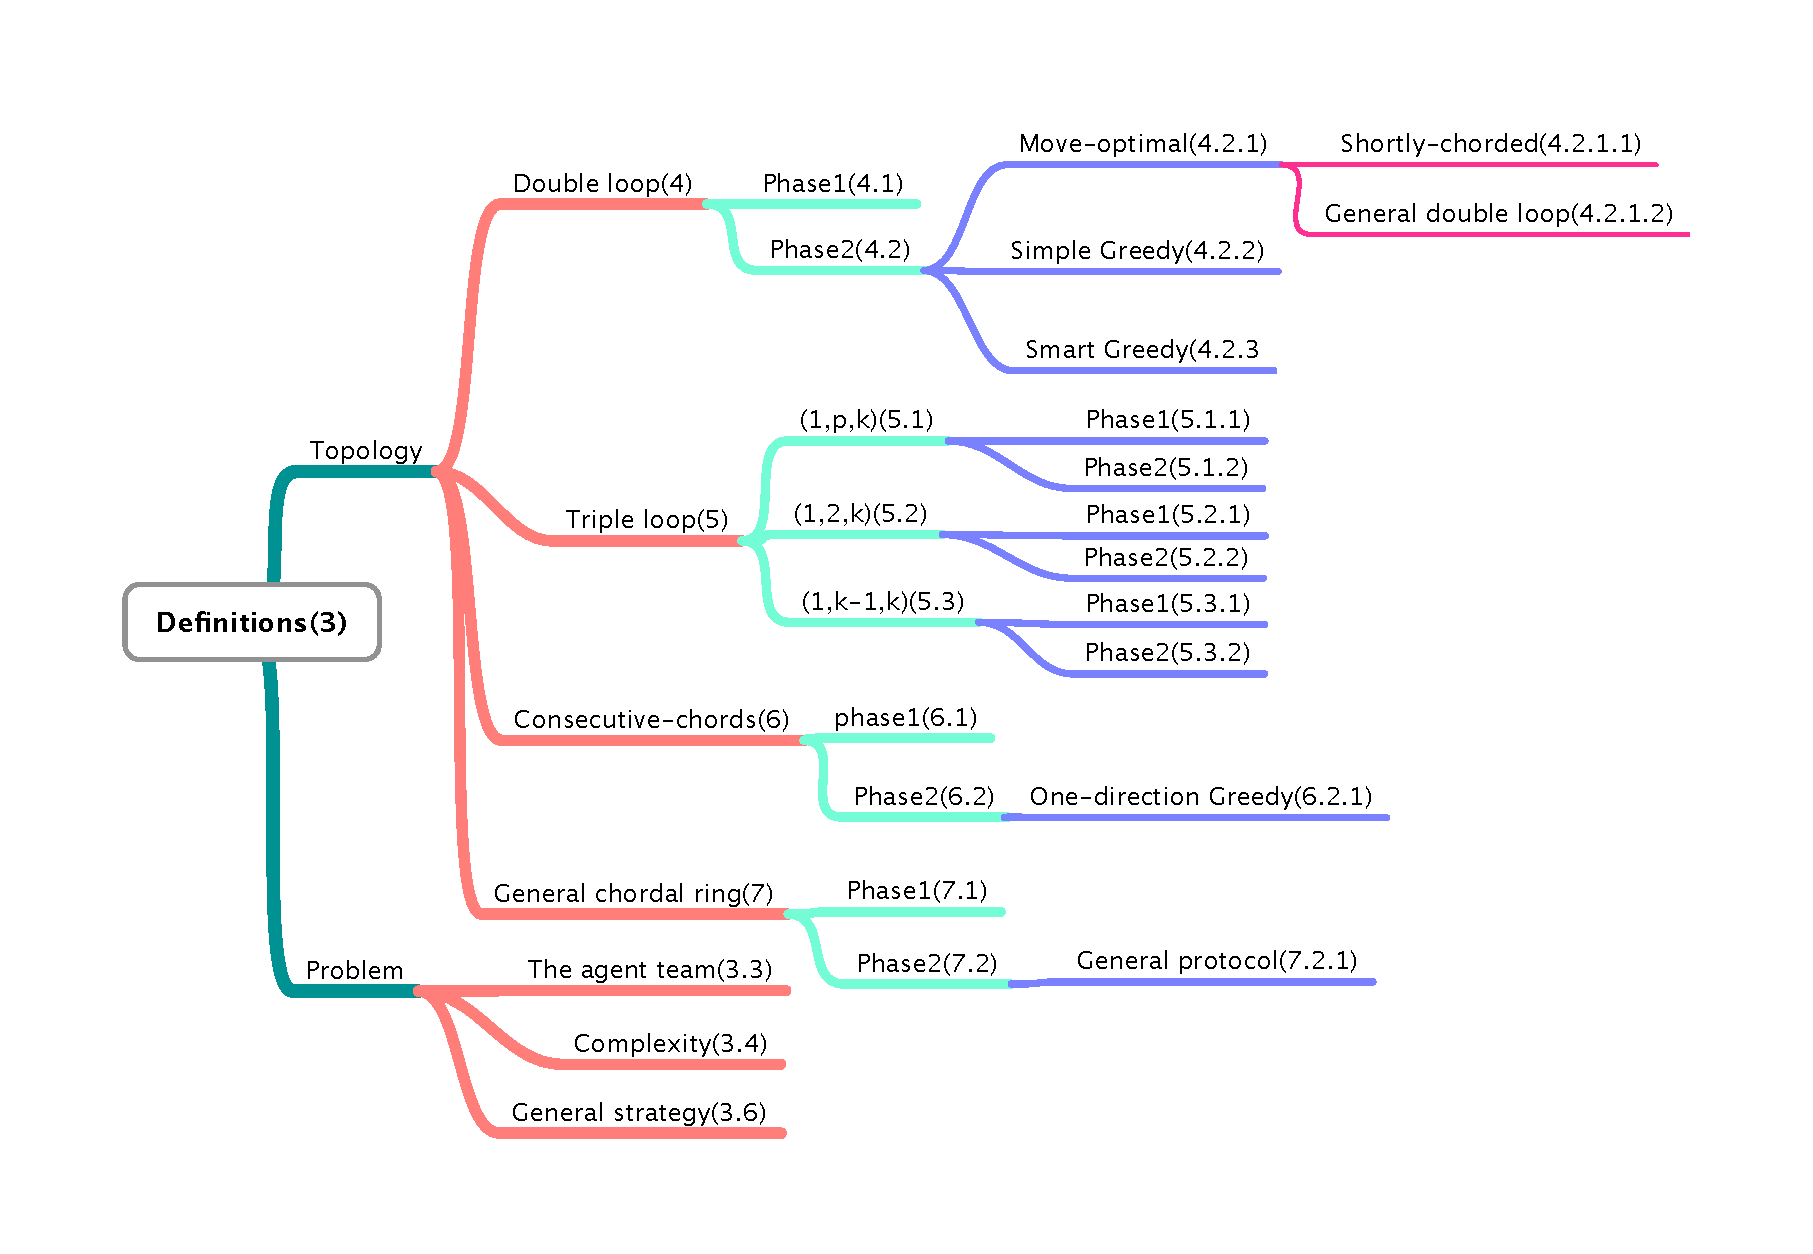
\includegraphics[width=1\textwidth]{figures/map2.pdf}
  \caption{A map showing the organization of the thesis}
\end{figure}

\end{comment}

%%%%%%%%%%%%%%%%%%%%%%%%%%%
\chapter {Literature Review}
\label{RW}
%%%%%%%%%%%%%%%%%%%%%%%%%%%
Mobile agents have been widely used in the field of distributed computing due to their features especially the mobility which allow them to migrate between computers at any time during their execution. A group of agents can be used to perform a various tasks, for example, network exploration, maintenance, and etc. However, the introduction of mobile agent tend to cause security problem, thus threatening the network. Various security issues and solution algorithms have been proposed by Flocchini and Santoro in \cite{security}. Generally, the threaten that the mobile agents cause are divided into two categories: in first case,the malicious agents can cause network nodes malfunction or crash by contaminating or infecting them (the harmful agent); in second case, the contaminated or infected hosts can destroy working agent for various malicious purposes (the harmful hosts). These two threaten trigger two problems: Black Hole Search (BHS) and Intruder Capture (IC) which will be introduced in the following sections. Then we review the BVD problem which deal with the decontamination of a harmful presence which cause the network node malfunction but leaves the network node clean when it is triggered and spreads to all its neighbouring nodes, thus increases it presences. In the section introducing BVD problem, we present the the abilities of mobile agents that has been proposed and different decontamination strategies based on different strategies.

\section{Black Hole Search, BHS}
The BHS problem assumes there is a BH or multiple static BHs residing at certain network nodes and will destroy any upcoming agents without leaving any detectable trace.The task is to use a team of agent to locate the black hole(s) and is completed when at least one agent survives and reports the location(s) of the black hole(s). Note that the solution is based on graph exploration and the goal can be reached totally depending on the sacrifice of some agents. In \cite{Das}, Das et al. considered a model for unknown environment with dispersed agents under the weakest possible setting, many exploration models and works were included in this article. The BHS problem has been widely studies in various topologies and settings: the timing is synchronous or asynchronous; the number of black hole(s) is known or unknown. For example: by Chalopin \cite{Das1,Das2} in asynchronous rings and tori, Dobrev et al. \cite{ Dobr} in arbitrary graph, \cite{Dobr1} in anonymous ring and \cite{Dobr2} in common interconnection networks...What is worth pointing out is that the number of BHs remains the same as it of the beginning, thus not causing harm to other sites of the network.


\section{Intruder Capture}
The IC problem assumes that there is an intruder moves with an arbitrary speed from node to node in the network and contaminate the sites it visits, the goal of which is to deploy a group of mobile agents to capture the intruder;the intruder is captured when it comes in contact with an agent. Note that the intruder does not cause any harm to the upcoming agents. It is equivalent to the problem of decontaminating a network contaminated by a virus while avoiding any recontamination. This problem is first introduced in \cite{Flocchini} and has been widely investigated in a variety network topologies: trees \cite{Flocchini, Flocchini1,treeintruder}, hypercubes\cite{Flocchini2}, multi-dimensional grids\cite{ Flocchini2}, chordal rings\cite{Flocchini3} etc. The studies of arbitrary graph has been started in \cite{Nisse,Nisse1}. Note that monotone is a critical principle in the solutions of IC problems.  

\section{Agent Capabilities}
Different capacities granted to the mobile agents have an impart on solving the BHS problem,IC problem and also the BVD problem.now we discuss these capabilities in the following section.

\paragraph{Communication Mechanisms} 
Mobile agents can communicate with each other only when they are in the same node in a network.Some essential communication methods have been studied in literature: whiteboard,tokens and time-out. In \cite{J.C, Dobr, Flocchini4, A.K}, the whiteboard model is used, which is a storage space located at each node and agents arriving there are able to read and write. In the token model, (see \cite{ J.C1, Flocchini4}), tokens are like memos of the agents which can be dropped off and picked by agents at nodes or edges. While the time-out mechanism can only be used in synchronous setting where each agent has a pre-determined amount of time. (see \cite{C.C, C.C1, J.C2}).

\paragraph{Knowledge of the topology} 
Different assumption of mobile agents' knowledge of the topology has an impact on solutions of some of the problems mentioned above, for example, the BHS problem. In \cite{Dobr}, Dobrev et al. present three types of topological knowledge in an asynchronous arbitrary network and show the results of the BHS problem based on different setting of the topology knowledge.

\paragraph{Other capabilities}
In some studies, agents are endowed with the visibility, which mean that they can see whether or not their neighbouring nodes are clean or contaminated (see \cite{M.Huang, M.Huang1}).They observe that the visibility assumption allow them to drastically decrease the time and move complexities in torus, chordal ring and hypercubes when dealing with IC problem. For example, in chordal ring $C_n\{d_1=1,d_2,...,d_k\}$, the number of agents, the time and the moves required in local model are $(2d_k+1)$, $3n-4d_k-1$, $4n-6d_k-1$ respectively, while in visibility model, they are $2d_k$, $\left \lceil \frac{n-2d_{k}}{2(d_{k}-d_{k-1})} \right \rceil$, $n-2d_k$. In torus , the number of agent, the time and the moves required are $2h+1$, $hk-2h$, $2hk-4h-1$ and in visibility model are $2h$, $\left \lceil \frac{k-2}{2} \right \rceil$, $hk-2h$ respectively. They also compare the complexity of both models in hypercubes, a algorithm requiring $\Theta$  ($n \over { \sqrt {log n}} $) number of agents and $O(n \log n)$ moves while the algorithm they propose in the visibility model requires $\frac{n}{2}$ agents and $O(n \log n)$ moves.

In \cite{Cai3}, the concept of {\em k-hop visibility} is presented. The agents have the {\em full topologies} if each of them have a map in their memory  of the entire network including the identities of the node and the labels of the edges. If a agent has {\em k-hop visibility}, then at a node {\em v} a agent can see the k-neighbourhood $N^{(v)}$ of {\em v}, including the node identities and the edge labels. Note that {\em Diam-hop} visibility is equivalent to full topological knowledge. 

Another interesting capability of agents is cloning which is introduced in \cite{M.Huang1}. Cloning is the capacity for an agent to create copies of itself. In this paper, they also discuss how the combination of different capacities reaches different optimal strategy in IC problem in hypercube. For example, the strategy is both time and move-optimal when visibility and cloning are assumed or when cloning, local and synchronicity are assumed. But the time and move-optimal strategy can be obtained at the expense of increasing the number of agents.
The last capability of agents be discussed is immunity which means that a node is immune from recontamination after an agent departs. Two kinds of immunity have been proposed:local and temporal. In local immunity, (see
\cite{Flocchini6,N.Santoro}, the immunity of a node depends on the state of its neighbouring nodes. More specifically, a node remains clean after the departure of an agent until more than half of its neighbours are contaminated. In the temporal immunity, a node is immune for a specific amount of time $(t)$. The node remains clean until time expires and becomes recontaminated if at least one of its neighbours are contaminated. In models without immunity assumption, a node becomes recontaminated if it has at least one contaminated neighbours.

\section{Black Virus Decontamination}
\subsection{Overview}
The BVD problem is first introduced by Cai at al. in cite{Cai}: A black virus is a  extraneous harmful process endowed with capabilities for destruction and spreading. The location of the initial BV(s) is known a priori. Like a BH, a BV destroy any agents arriving at the network where it resides. When that happen, the clones of the original BV spread to all it neighbouring nodes and remain inactive until an agent arrives. The BVD problem is to permanently remove any BVs in the network using a team of mobile agents. They proposed that the only way to decontaminate a BV is to surround all its neighbouring nodes and send an agent to the BV node. In this case, the node where the original BV resides is clean and all its clones are destroyed by the guarding agents in its neighbouring nodes.They have presented different protocols in various topologies: q-grid, q-torus, hypercudes in \cite{Cai} and arbitrary graph \cite{Cai1}. A basic idea of implementing the decontamination has also been propose by them assuming that the timing is asynchronous which divides the whole decontamination process into two part: '{\em shadowed exploration}' and '{\em surround and eliminate}'. In order to minimize the spread of the virus, they use a '{\em safe-exploration}' technique which is executed by at least two agents: the {\em Explorer Agent} and the {\em Leader Explorer Agent} who both residing at a safe node {\em u} at the beginning, for example,the homebase. The {\em Explorer Agent} moves to a node {\em v} to explore it and it needs to return to node {\em u} to report the node {\em v} is safe. The {\em Leader Explorer Agent} determines if the node {\em v} is safe or not by {\em Explorer Agent}'s arriving or a BV's arriving. If node {\em v} is safe, both of them move to node v. For the purpose of insuring monotonicity, at any point in time the already explored nodes must be protected so they are not be recontaminated again. After the BV is detected, the '{\em surround and eliminate}' begins. In this phase, some agents are employed to surround the new-formed BVs (the clones of the original BV) then some agents are sent to the clones to permanently destroy them. This is called the '{\em Four-step Cautious Walk}' and is widely used in BVD problem with synchronous setting. Also, BVD problem in chordal ring has been discussed in
\cite{Alotaibi}.

\subsection{BVD in different topologies}
Protocols regarding to BVD problems in grid are BVD-2G and BVD-qG which deal with BVD problems in 2-dimensional grid (meshes) and q-dimensional grid respectively. BVD-2G performs a BV decontamination of a 2-dimensional grid of size $n$ using $k=7$ agents and 3 casualties, within at most $9n+O(1)$ moves and at most $3n$ time. While protocol BVD-qG performs a decontamination of a q-dimensional grid of size $d_1\times d_2 ...\times d_q$ using $3q+1$agents and at most $q+1$ casualties, within at most $O(qn)$ moves and at most $\Theta$($n$) time. Algorithm to decontaminate the BV in a q-dimensional torus,called BVD-qT uses $4q$ agents with 2 casualties with at most $O(qn)$ moves and $\Theta$($n$). Protocol BVD-qH is to perform a BV decontamination of a q-hypercube using $2q$ agents and $q$ casualties with at most O($n\log n$) moves and $\Theta$($n$). In arbitrary graph (see \cite{Cai1}), two protocols are presented: GREEDY EXPLORATION and THRESHOLD EXPLORATION. In these two protocols, $\Delta +1$ agents are needed and both of the protocols are worst-case optimal with respect to the team size. Though the protocols are described for a synchronous setting, they easily adapt to asynchronous ones with an additional O($n$) moves for the coordinating activities. An advantage of these protocols is that the agents can use only local information to execute the protocol. Another interesting fact based on these two protocols is that both GREEDY ROOTED ORIENTATION and THRESHOLD ROOTED ORIENTATION produce an optimal acyclic orientation rooted in the homebase.

In \cite{Alotaibi}, solution for BVD in chordal ring is discussed. In Alotaibi's thesis, she discuss solutions based on different kinds of chordal ring: double loops, triple loops, consecutive-chords rings and finally general chordal ring. In double loops, she proposed three strategies in elimination phase and the upper bound of moves is $4n-7$ in the whole protocol and a maximum of 12 agents are employed.In triple loops, she discusses two classes of chordal ring: $C_n(1,p,k)$ and $C_n(1,k-1,k)$. In any triple loop $C_n(1,p,k)$, a maximum of $5n-6k+22$ moves and 24 agents are needed for the decontamination while in any triple loop $C_n(1,k-1,k)$, a maximum of $5n-7k+22$ moves and 19 agents are needed. Finally in the consecutive-chords ring, a maximum of $(k+2)n-2k-3$ moves and $4k+1$ agents are needed. She described the decontamination strategies in synchronous setting but only with a cost of $O(n)$ moves can the strategies be used in asynchronous setting.

Chapter 2 end 


%\section{Decontamination}

%Because of network connectivity, a moving object can contaminate an entire network, resulting in dysfunctional performance. This scenario is considered to be one of the most critical threads in network security (ie.,  viruses and how they attack devices on the Internet). As a result, there is a need for a cleaning and protecting process ({\em Decontamination}). This problem has been extensively studied in graph theory under several names: graph search, intruder capture and decontamination. This problem was first introduced in 1967 by \cite{bre4}. The decontamination process can be conducted internally or externally. Internal decontamination allows a node to perform the task without external help. In other words, the nodes are able to decontaminate themselves locally. For example, running an Anti-virus program on an infected device could rid that device from viruses it got from the Internet. On the other hand, external decontamination requires external intervention, such as mobile agents. An agent decontaminates infected nodes by passing through them, yet the nodes are vulnerable to recontamination once the agents depart. 


The Mobile Agents Model is a form of external decontamination in which moving agents are used to disinfect a contaminated network.
The mobile agents must decontaminate the network in a way that prevents recontamination. In this model, nodes have three states: contaminated, decontaminated or guarded. A node is decontaminated once an agent passes through it, guarded once an agent resides in it and otherwise contaminated. Initially, all nodes are contaminated with the exception of the homebase which is guarded. This model has many variations and parameters that have a significant impact on the overall complexity. As a result, there are many protocols and strategies that handle this problem in various topologies. These protocols were designed to be {\em monotone}, that is, once a node is decontaminated, it can not be re-infected.

Usually, the complexity of such protocols is measured by the number of agents used in the decontamination process, the number of moves the agents make and the amount of time needed to decontaminate an entire network.

The following variations have a significant impact on protocol performance and complexity: synchronicity, agent capabilities and topological characteristics.
\subsection{Synchronicity}
For synchronous execution many papers address the problem of decontamination where agents synchronize their movements in such a way that the explored nodes never get re-contaminated  (see \cite{lucetal22,floc21,baretal24}). In the case of asynchronous execution, there is a need for a coordinator who organizes other agents, ensuring that all agents are in the correct positions before starting a new step (see \cite{floetal13,lucetal22,floetal20,floetal19,floetal17}).


\subsection{Agent Capabilities}
In this problem, agents have been given certain capabilities including cloning, visibility and immunity.

\paragraph{ Visibility.}  Some studies have granted agents the visibility, which is the ability to see whether the neighbouring nodes are clean or contaminated (see \cite{floetal17,floetal20}). Some studies have only employed the local model in which agents only know the information (state, ports) for the node in which they reside (\cite{floetal19,floetal17,floetal20}). Visibility impacts complexity since the agents are able to move in an autonomous fashion, without the need for coordination. In \cite{floetal17}, Flocchini et al. demonstrate that to decontaminate a chordal ring $C_n\{d_1=1,d_2,...,d_k\}$ in the local model, the number of agents required is $(2d_k+1)$, while in the visibility model, the number of agents required is $(2  d_k)$.

 In \cite{floetal20}, Flocchini et al. compare the complexity of  decontaminating a hypercube in both models. In the local model, they propose an algorithm that requires  $\Theta$  ($n \over { \sqrt {log n}} $) number of agents and  $O(n \log n)$  moves. In the  visibility model, they propose an algorithm that requires ($n\over2$) agents and $O(n \log n)$ moves.



\paragraph{ Cloning.}
Cloning refers to an agent's ability to make copies of itself. This feature would reduce the number of moves but would not produce an optimal number of agents. In \cite{floetal20}, Flocchini et al. study the impact of the cloning feature on the decontamination of a hypercube. They demonstrate that using cloning, the number of moves is drastically reduced: ($n-1$) in both the visibility and local models.


\paragraph{ Immunity.}
Immunity means that a node is immune from recontamination after an agent departs. In the literature, there are two types of immunity: local and temporal. In local immunity, the immunity of a node is determined by the state of its neighbours. For instance, a node stays clean after the departure of an agent unless the majority of its neighbours are contaminated. If the majority of its neighbours are contaminated, that node gets re-contaminated. In other words, the immunity level in this model is about half of the node’s degree. If the contamination reaches more than half, the node gets re-contaminated (see \cite{lucetal22,floc21}). In temporal immunity, a node is immune for a specified amount of time $(t)$. After the departure of an agent, the node is clean for $t$ time regardless of the state of its neighbours. After the time elapses, the node is vulnerable to recontamination if it has at least one contaminated neighbour (see \cite{floetal13}). The two types of immunity provide a network with some resistance to recontamination.  In the absense of these two models, the immunity of the nodes is nil, meaning that the node can be recontaminated if any of its neighbours are contaminated.



\subsection{Topologies}

The mobile agent decontamination model has been studied in various topologies. In this section we list the results of decontamination protocols in some common topologies.

 
\noindent{\bf Tree.}  
Many researchers have studied the decontamination process in trees. The basic strategy for decontaminating a tree is to divide the tree into sub-trees starting from a single homebase (the root), see \cite{floetal13,lucetal22}. 

The best case scenario in terms of the number of agents required occurs when the homebase is the first or last node and we have a line that requires one agent for decontamination. If the homebase is any other node, we require two agents. The worst possible case is the decontamination of a complete binary tree.


In \cite{lucetal22}, Luccio et al. consider an asynchronous environment, continuous search, visibility mode, local immunity, single homebase, and a monotone strategy. In order to enforce local immunity there are three basic rules controlling agent departure from a node. If the number of clean neighbours is lower than half of the total number of neighbours (i.e. the majority), the agent does not depart. If the number of clean neighbours is equal to half of the total number of neighbours, the agent only moves to a contaminated neighbour. If the number of clean neighbours is greater than half of the total number of neighbours, the agent moves to any neighbour.
To identify the minimum number of cleaning agents, this paper divides trees into two classes: trees with degree $d \leq 3$ (e.g. binary tree, line) and general arbitrary trees.
\begin{itemize}

\item Trees with degree $d \leq 3$ can be decontaminated using a maximum of two agents,
%Obviously, we need only one agent to decontaminate a line; also we need only one agent to decontaminate any n-node binary tree, 
while the number of moves is $(2(n-1) - diam)$, where $diam$ represents the diameter. 
\item For general arbitrary trees with degree $d >3$, this paper introduces the state of stability. A node x is stable if it satisfies the following two conditions: x is immune to recontamination whether it is guarded or not, and the majority of its children are stable. 
The authors use these conditions to determine the minimum number of cleaners needed to keep a node stable. As a result, we can determine the minimum number of agents required to decontaminate the entire tree. Any lower bound on the minimum number of agents needed to stabilize x provides a lower bound on the minimum number of agents needed to decontaminate a tree rooted in the homebase. In this protocol, the agent stabilizes the root and then recursively moves to unstable nodes and stabilizes them until all nodes are stable. The number of moves in this protocol is not proven. This study demonstrates how local immunity improves complexity (minimum number of cleaners), especially in a binary tree.
 \end{itemize}
In \cite{floetal13}, the authors consider a synchronous environment, continuous search, temporal immunity (i.e. $t>0$), single homebase and a monotone strategy. In this case, any node is immune from recontamination when it is guarded and during the immunity time $t$ after the agent leaves. Therefore, agents can move back and forth during period t. In other words, an agent can leave a node and traverse a path of length up to t/2 and go back to that node without worrying about recontamination. Using this property, the Depth-First traversal strategy, and a decontaminating leader (i.e., an agent), this paper demonstrates that a tree requires at least $2h\over(t+1)$ agents, where $h$ is the height of the tree, and $t$ is the immunity time. We can see that the temporal immunity has a significant impact on the process of decontamination. 


\noindent{\bf  Hypercube.}
The hypercube is thoroughly studied in \cite{floetal20}. This paper discusses several strategies for decontaminating a hypercube. The authors consider the local and visibility models, with and without cloning as we mentioned in the previous section.

%For the first strategy, the authors assume local model, asynchronous environment, single homebase, continuous search, and monotone strategy. This strategy relies on the existence of a coordinator (agent) that directs how the other agents move since the agents don’t have the capability to see the states of neighbours. This decontaminating strategy is performed on the broadcast tree of the hypercube level by level.
%It is proven that this strategy requires number of agents= Θ(n/(log n)1/2) ,and number of moves= O(n log n), where n is the number of nodes.
%The second strategy is the same as the first one except that this strategy considers the visibility model. This strategy uses (n/2) agents and O(n log n) moves to decontaminate the network. We can notice the drop in the number of agents in the visibility model. Lastly, the third strategy considers the visibility model and cloning. However, in this case no coordinator is needed. In this protocol, Initially, one agent starts from the homebase, then it clones agents as many as the number of dimensions -1, and send one agent through each link. After an agent cleans a node, it clones enough agents to clean all neighbors that are not clean or guarded. As a result the number of moves performed by agents is decreased to (n-1), where the minimum number of agents required for monotone decontamination is n/2. The following table shows a comparison between the previous three strategies in terms of complexity. Hence the table shows the time complexity.






\noindent{\bf Mesh.}
As seen in \cite{floetal19}, to decontaminate a mesh (grid) of $M\times N$ nodes, there two possible strategies. The authors assume an asynchronous environment, continuous search, single homebase, and monotone protocol. In the first strategy the authors use the local model in which the agents cannot see neighbouring states but have the ability to exchange information using whiteboard. In this strategy there is a need for a synchronizer that coordinates the protocol execution. Beginning from the homebase, $M$ agents (except one agent that remains at the homebase) move south in order to guard each node in the first column. The synchronizer then coordinates the moves of all agents in such a way that all the agents are moving east at the same time.  This process goes on column by column until the whole graph is decontaminated. This protocol requires $M+1$ agents and ${M^2+4MN-5M-2}\over 2$ moves. In the second strategy, the authors use the visibility model, eliminating the need for a synchronizer. In this case, agents depend on what has been written in the whiteboard to decide the next step. This strategy requires $M$ agents (no synchronizer here) and ${M^2+2MN-3M}\over 2$ moves.

In the previous two protocols, the authors assume a mesh M×N, where $M\leq N$, so the protocols carry on column by column. In the case of  $N < M$, it is better to proceed row by row to obtain a lower number of agents.

\noindent{\bf Tori.}
A torus $h\times k$ ($h<=k$) is a mesh where the nodes in the last row are connected to nodes in the first row, and nodes in the first column are connected to nodes in the last column. In order to decontaminate a torus we can use the strategies used to decontaminate a mesh with some slight modifications.  In \cite{floetal17}, Flocchini et al. use strategies similar to those used for the mesh. Instead of deploying agents to cover one column, agents are deployed to cover two successive columns. One column of agents then stays to guard the nodes from recontamination while the other column of agents moves through the torus. In the local model there is a need for a synchronizer. The complexity of this strategy is $2h+1$ agents and ($2hk-4h-1$) moves. In the visibility model, there is no need for a synchronizer, and the complexity is $2h$ agents and ($hk-2h$) moves. In \cite{lucetal22}, the authors demonstrate that in order to decontaminate a  k-dimensional tori ($k>2$) in the presence of local immunity, we need at least $2k$ synchronous agents and ($n+2k-2k-2$) moves.

\noindent{\bf Rings.}
When we have a ring  it is easy to find the minimum number of agents required for monotone decontamination. 

In the local model, two agents are sufficient to perform the decontamination if they start from a single homebase and move in opposite directions until they are reunited. The number of moves would therefore be n, where n represents the number of nodes, if we assume that an agent needs one time unit to traverse a link. In the visibility model, the two agents move in opposite directions until they reach two consecutive nodes. The number of moves is therefore $n-1$ (see  \cite{lucetal22}).


\noindent{\bf Chordal Rings.}
In \cite{floetal17}, Flocchini et al. provide the results of decontaminating a chordal ring $C_n\{d_1=1,d_2,...,d_k\}$ using the local and visibility models. In the local model, the complexity required to decontaminate the chordal ring using  asynchronous execution is $ (2d_k+1)$ agents and $4n-6d_k-1$ number of moves. In the visibility model, the number of agents is $(2  d_k)$  and the number of moves is ($n-2d_k$). 





%\section{Fault Tolerance in Chordal Rings}

\section{Black Virus Decontamination}
This term was initially introduced by Cai el al. in \cite{caietal18}. The {\it Black Virus} ($BV$) is a hostile node that resides in an unknown location, causing the destruction of any visiting mobile agent. The black virus also causes more damage by moving to neighbouring nodes. Therefore, we need a strategy to locate the hostile node and to disinfect the entire topology from its spread.
In \cite{caietal18}, the authors present the {\it Black Virus} (BV) threat by combining the statical feature of the {\it Black Hole} and the mobility feature of the {\it Intruder Capture}. They also propose a solution to the $BVD$ problem using a team of mobile agents. 

The authors assume that there is initially only one $BV$ in the network. Like $BH$, the location of $BV$ is unknown a priori and the $BV$  stays inactive (unharmful) unless it is triggered. The $BV$ is activated when a mobile agent arrives at its location. The mobile agent is then destroyed and the $BV$ clones itself into as many $BV$s as its number of degrees. The copies retain the same features as the original and each copy moves to a neighbouring node and remains inactive until triggered. According to \cite{caietal18}, the \bv is only deactivated when it moves to a node that is occupied by an agent. To the best of our knowledge, this problem has only been studied by Cai et al. in \cite{caietal18}.

In \cite{caietal18}, the proposed protocol consists of two phases: '{\em shadowed exploration}' and '{\em surround and eliminate}'. As the names suggest, the first phase involves exploring  the network, locating the \bv and triggering it. The second phase involves surrounding the newly created $BV$s and then triggering them to remove them from the network. This protocol is monotone, meaning that once a node is explored, it is immune from recontamination. The measures of efficiency considered include:  the spread ($spread$), the number of agents ($size$) and the number of moves.
The $BVD$ problem is solved when the network is completely decontaminated and at least one agent survives.
 The authors conduct their research using common topologies such as rings, multi-dimensional grids, multi-dimensional tori and hypercubes.

\noindent{\bf Ring(R).} The authors demonstrate that, regardless of the number of nodes ($n$), the monotone protocol requires ($size(R)= 4$) and ($spread(R)= 2$). It is possible that these results are not quite accurate. If the  \bv resides in node $n-1$, we either have a non-monotone protocol in which an explored node gets contaminated or  less complexity where ($size\leq 4$) and ($spread \leq 2$).

\noindent{\bf Grid(G).}The paper considers a 2-dimensional grid and a q-dimensional grid. In a 2-dimensional grid of size $d_1\times d_2$, they prove that regardless of $n$ their proposed optimal algorithm would cost ($spread(G)=3$), ($size(G)=7$), and at most ($5n+O(1)$) number of moves . While in a q-dimensional grid, the complexity would be ($spread(G)=q+1$), ($size(G)=3q+1$), and at most ($O(qn)$)  number of moves. 

\noindent{\bf Torus(T).} According to the protocol, decontaminating a q-dimensional torus from $BV$  requires  ($spread(T)=2q$), ($size(T)=4q$) and  ($O(qn)$) moves.

\noindent{\bf Hypercubes(H).} According to the protocol, decontaminating a hypercube from $BV$s requires ($spread(H)=3$), ($size(H)=6$) and at maximum of $34$ moves.
 

 










%%%%%%%%%%%%%%%%%%%%%%%%%%%
\chapter {Definitions and Terminology}
\label{PM}
%%%%%%%%%%%%%%%%%%%%%%%%%%%
\section{Model}
\subsection{Network, Agent, Black Virus}

\noindent{\bf Network} The environment in which mobile agents operate is a network modelled as simple undirected connected graph with $n = \left |V\right |$ nodes (or sites) and $m = \left |E\right |$ edges (or links). We denote by $E (v)\subseteq E$ the set of edges incident on $v\in V$, by $d (v) = \left|E (v)\right|$ its degree, and by$\Delta(G)$ (or simply $\Delta$) the maximum degree of G. Each node v in the graph has a distinct $id(v)$. The links incident to a node are labelled with distinct port numbers. The labelling mechanism could be totally arbitrary among different nodes; without loss of generality, we assume the link labelling for node $v$ is represented by set $l_v =1,2,3,...,d(v)$. 

\noindent{\bf Agent} A group of mobile agents are employed to decontaminate the network. The agent is modelled as a computational entity moving from a node to neighbouring node. More than one agents can be at the same node at the same time. Communication among agents occurs at this time; there are no a priori restrictions on the amount of exchanged information.When the agent arrives at a node, it can leave message on that node and read massage on that node. Information on the nodes can be set (writing the information on a white board) at the beginning of the exploration, so when the agent reach the node, it can update the information on the white board or update its own memory by learning the information on the white board.  We assume that all the agent' s moves follow the same clock. Also, agents are endowed with 1-hop visibility which means at a node {\em v}, it can see the labels of the edges incident to it and the identities of all its 1-hop neighbours. 

\noindent{\bf Black Virus}
In {\em G} there is a node infected by a black virus (BV) which is a harmful process endowed with reactive capabilities for destruction and spreading. The location of the BV is not known at the beginning. It is not only harmful to the node where it resides but also to any agent arriving at that node. In fact, a BV destroy any agent arriving at the network site where it resides, just like the black hole. Instead of remaining static as the black hole, the BV will spread to all the neighbouring sites leaving the current node clean. The clones can have the same harmful capabilities of the original BVs (fertile) or unable to produce further clones(sterile). A BV will be destroyed if and only if the BV arrive at a node where there is already an agent. Thus, the only way to eliminate the BV is to surround it completely and let an agent attack it. In such situation, the attacking agent will be destroyed while the clones of the original BV will be permanently eliminated by the agents residing the neighbouring nodes of the original node. We assume that at the same node, multiple BVs (clone or original) are merged. More precisely, at any time, there is at most one BV at each node. 
Another important assumption is that when a BV and an agent arrive at an empty at the same time, the BV dies and the agent survive remaining unharmed.

Also, in this thesis, we assume that when a BV is triggered, it take negative time for its clones to spread to all its neighbour. More specifically, when a BV is triggered by an agent at T($t_i$), then in T($t_i$), all the neighbours of this agents(if exist) receive the clones of it. The reason we make this assumption is that when we try to eliminate the new formed BVs parallelly in the chordal ring and assume that it takes one unit of time for both the agents and the BV to move from one node to another, then we are faced with a tricky situation: if the sites of two(or more) agents are connected, after these two clones are triggered(we send an agent to each of them to permanently destroy them), one of their clones spread to another site and since the agents sent to contaminate them die, these two sites are empty when the second round clones arrive, which make the decontamination invalid.
While with the assumption, the tricky situation can be easily solved: after the two clones are triggered, one of their clones spread to another site and both the original clone and the second round clone are destroyed by the agent.



Summarizing, there are five possible situations when an agent arrive at a node {\em v}:
\begin{itemize}
\item agents arrive at a node which is empty or contains other agents, they can communicate with each other and the node {\em v} is clean.
\item agents arrive at a node which contains a BV,the clones of the BV (BVC) spread to all the neighbours of {\em v} and the agent dies, leaving node {\em v} clean.
\item A BVC arrives at a node which is empty or there is already a BV: the node becomes/stays contaminated; it merges with other BVs.
\item BVCs arrive at a node {\em v} which contains one or more agents, the BVCs are destroyed but the agents are unharmed.
\item A BVC and an agent arrive at an empty node at the same time, the BVC dies while the agent remains unharmed. 
\end{itemize}

\subsection{Problem, Cost}
The BLACK VIRUS DECONTAMINATION (BVD) problem is to permanently remove the BV, and its clones from the network using a team of mobile agents starting from a given node, called home base(HB). The solutions where the agents explore the network sequentially have been proposed in some classes of topologies. chordal rings, hypercubes and arbitrary graph. In this thesis, we are interested in parallel strategies in BVD problem: instead of exploring the network in sequence, we explore it in parallel; in chordal ring, we also propose a parallel solution to surround the clones of the original BV. 
In this thesis, the efficiency measurements we have are: {\em spread} of BV (also measures the number of agents {\em casualties}; the {\em size} of the team, i.e, the number of agents employed by the solution; total working time(TWT) (calculated by multiplying the {\em size} of the team and the time cost by the solution. Note that TWT does not contains any practical meaning but exist only as a measurement. We propose TWT to compare more fairly the time of two protocols when the number of agents is different.

\subsection{Monotone, Synchrony}
A desirable property of a decontamination protocol is to prevent the nodes which been explored or cleaned by mobile agent from being recontaminated which will occur if the clones of the BV are able to move to a explored node in absence of agent. A BVD protocol with such property is called monotone. Monotone property is the necessary condition for spread optimality.

Asynchrony refers to the execution timing of agent movement and computations. The timing can be {\em Synchronous} or{\em Asynchronous}. When the timing is synchronous, there is a global clock indicating discrete time unit; it takes one unit for each movement (by agent or BV); computing and processing is negligible. When we have asynchronous agents, there is no global clock, and the duration of any activity (e.g., processing, communication, moving) by the agents, the BV, and its clones is finite but unpredictable. In this thesis, all our protocols work in synchronous setting.

\section{ General strategy}
Following the solution in sequential case, we decomposed the BVD process into two separate phase: {\em Shadowed Exploration} and {\em Surrounding and Elimination}. The task of the first phase is to locate the BV and the second phase is to decontaminate the BV and its clones. Apart from these two basic phase, we have initialization which is to deploy the agents properly at the beginning of executing the protocol because we explore the network in parallel, and the arrangement of the agents is crucial to successfully execute the protocol. 

\noindent{\bf Phase1: Shadowed Exploring}  Agents employed are divided into two group: shadowing group and exploring group, and the number of agents in two group is the same. For convenience, we call the agent in the shadowing group the shadow agent ({\em SA} and those in the exploring group the exploring agent {\em EA} (one {\em EA} is accompanied by one {\em SA}. As the name indicated, agents in exploring group explore the network and the agents in shadowing group follow the agents  protecting the node which have been explored. More precisely, at $T_1$, EA moves to node {\em v}; at $T_2$, SA moves to node {\em v} and EA moves to node {\em u} supposing that node {\em v} is clean. 

\noindent{\bf Phase2: Surrounding and Elimination}
In this phase, since we already know the position of the BV, we employ agents to surround all the neighbours of the BVCs. Once all the agent arrive the proper positions( all the neighbours of the BVCs are guarded), we employ another group of agents (the number of them is equal to the number of BVCs) to move to the BVCs, thus permanently destroy them. Usually, some of the agents moving to the neighbours of the BVCs are from the shadowing group and exploring group because in this way we can save the number of agents used in the whole protocol. Note that not all the agents are informed when the BV is detected. More specifically, only the agents who receives the clones know the existence of the BV, and other agents keep moving in the network. In some simple topologies, such as meshes and torus, the second phase begins when the BV is detected since the number of agents are enough to proceed the second phase. In some more complicated topologies, for example, the chordal ring which we discuss later, we take some other measures to call back enough number of agents to finish the second phase.
\section{Evaluation Criteria}
For each of our strategy, we compute the number of agents, the number of movements, the time and the casualties.  In addition, we propose another cost measure which combines all the criteria mentioned above (Cost Function Measurement). In this thesis, we propose parallel strategy which aim at reducing the execution time and casualties. We reach this purpose at the cost of employing more agents to explore the graph parallelly. Unlike the sequential strategy which use only one agent, the parallel strategy are more flexible because you can adjust the strategy based on your resource (the number of agents, the time,\ldots). Generally, the more agents we employ to explore the graph, the less time we use in the shadowed exploration phase( the number of casualties may reduce at the same time), so there are some tradeoff we should make when we want to use the parallel BV decontamination strategy in practice. Now we introduce the general idea of the Cost Function Measurement.
Let's denote by $w$ the number of agents we employ in the strategy, by $x$ the number of movements, by $y$ the time and by $z$ the casualties. Additionally, we introduce three useful function: $Cost_{AgentNumber}(w)$ which given the number of agents employed in the strategy, returns the overall cost of these agents; $Cost_{Movements}(x)$ which given the number of movements needed to complete the strategy, returns the overall cost of the movements; $Cost_{time}(y)$ which given the time required to finish the protocol, returns the overall cost of the time; $Cost_{casualty}(z)$ which given the casualty of the strategy, returns the overall of the casualties. Then the Cost Function $C(w, x, y, z)$ can be presented as $C(w, x, y, z)=C(Cost_{AgentNumber}(w), Cost_{Movements}(x), Cost_{time}(y), Cost_{casualty}(z))$.
Users can build their own function to fit the specific scenario. For example, if the user care more about the time cost, then they can increase the weight of the time; they can also adjust each subfunction to simulate the practical situation. The simplest model is the liner function. More specifically, the cost functions can be expressed as below:\\
\begin{equation}
\left\{
\begin{aligned}
&C(w, x, y, z)=Cost_{AgentNumber}(w)+Cost_{Movements}(x)+Cost_{time}(y)+Cost_{casualty}(z)\\
&Cost_{AgentNumber}(w)=\alpha w+\alpha _1\\
&Cost_{Movements}(x)=\beta x+\beta _1\\
&Cost_{time}(y)=\gamma y+\gamma _1\\
&Cost_{casualty}(z)=\delta z+\delta _1\\
&w, x, y, z\in \mathbb{Z}\\
\end{aligned}
\right.
\end{equation}
In this function we can see that the user view the four factor evenly (the coefficients of the four subfunctions are the same which are ``1''), and the cost of each item( agents, movement, time, casualty) increase linearly with their independent variable. We use this liner model to analyze some of our strategies. Note that the function we present here are for the purpose of explaining how to use the function method to analyze the BVD strategies, the function itself can be adjust by the users based on the practical situation.
We simply compare the overall cost of different strategies for the same problem and assume that the strategy with the minimum cost is the best solution for the users.  
\section{Conclusion}
In this Chapter, we presented the model of our problem and also some important terminologies. Also we described a general strategy for our problem depending on particular setting: synchronous timing, parallel strategy... In the next chapter, we discuss the parallel strategies in BVD problem in two simple topologies: meshes and torus. 







 





%%%%%%%%%%%%%%%%%%%%%%%%%%%
\chapter {Parallel Black Virus Decontamination in Meshes}
\label{DL}
%%%%%%%%%%%%%%%%%%%%%%%%%%%
 
\section{Introduction}
In this chapter, we discuss parallel strategy on BVD problem in grid and tori. In the sequential strategy ({\em BVD-2G}) for 2-dimensional grids which are meshes, an ``explorer agent ''and a ``leader explorer agent'' are sent to explore the graph and locate the BV. They traverse the mesh in a snake-like fashion column by column following the ``casual walk''. In the sequential protocol ({\em BVD-qG}) for q-dimensional grids, the grid is partitioned into $d_1\times\ldots\times d_{q-2}$ 2-dimensional grids of size $d_{q-1}\times d_q$, and each 2-dimensional grid is explored using the shadowed traversal technique as described in the 2-dimensional grids. Similarly, in the protocol ($BVD-qT$) for q-dimensional torus, the torus is partitioned into $d_1\times \ldots \times d_{q-1}$ ring of size $d_q$. The exploration procedure traverses a ring and, when back to the starting point, proceeds to another ring, with a neighbouring starting point. After locating the BV, agents surround the new formed BVs sequentially and eliminate them. These strategies are simple to follow, but at the same time they are not time-efficient. Now we consider that if more than two agents are allowed to participate in the exploring phase and we focus on decreasing the time cost in the exploring phase and the number of casualties, how to design a new strategy so that the we are able to reach the destination with acceptable cost (the increasing number of agents used in the exploring phase).\\
The general idea is simple, we will employ a group of agents and place them in a specific array at the beginning. Informally, in the shadowed exploration of our strategy in 2-dimensional grid({\em PBVD-2G}), q-dimensional grid({\em PBVD-qG})and tori({\em PBVD-qT}), the agents who are employed to explore the graph stay in that array and that ``agent array"  traverse that graph in the shadowed exploration. Note that after the BV is triggered, not all the agents automatically enter the elimination phase but only the agents who know the existence of BV, but in some cases, the number of agents knowing the existence of BV is not enough for surrounding and eliminating the BVs, so in the elimination phase, our strategies employ some agents who receive the clones of the original BV(thus knowing the existence of the BV) to notify some other agents to participate in the elimination phase. 
Also, we compare the number of agents, the time cost, the number of movement and also the casualty between each of our strategy and the sequential strategy.

\section{Parallel BV Decontamination of Grids}
\subsection{Base Case:2-Dimensional Grid}
A 2-dimensional grid (which is a mesh) of size $d_1\times d_2$ has $n=d_1\times d_2(d_1>2,d_2>2)$ nodes. Without loss of generality, let $d_1<d_2$ and let the node of {\em M} be donated by their column and row coordinate ($x_1$,$x_2$), $1\leq x_1 \leq d_1$, $1\leq x_2 \leq d_2$. Observe that in a mesh, we have three types of nodes: \textit{corner} (entities with only two neighbours), \textit{border}(entities with three neighbours), and \textit{interior}(with four neighbours).  Our strategy follows two phases: shadowed exploration and elimination. In the first phase, the network is traversed until the location of the BV is determined. That location is clear after the visit while all of its unprotected neighbours have become BVs. Actually, in $PBVD-2G$, there are only one new formed BV. In the second phase, new formed BV is surrounded and permanently eliminated. Note that when we say the second phase starts, we actually mean that those agents knowing the existence of BV start to surround the BV, or notify some other agents, and then eliminate the BV, but not mean that all the agents enter this phase. There are two significant differences between $PBVD-2G$ and the sequential strategy: the number of agents employed in the exploration phase; the route of agents in the exploration phase. We also give the routes of agents in the elimination phase. 

\noindent{\bf Shadowed Exploration Phase} \\

As we introduce above, we should place the agents in a specific array at the beginning and then let them explore the graph. Now let us consider how to arrange them at the beginning and how to design the routes for them to explore the graph. We prefer to place the agents at the borders (or the corners) of the mesh because in this way we can reduce the casualties. For the same purpose of reducing the casualties, we prefer to arrange all the agents in a array so that when one of the exploring agent trigger the BV, the exploring agents and shadowed agents guide as many neighbours of the BV as possible. In another word, we want all the agent explore the graph in one direction but not from different direction. With these two principles, our strategy in the shadowed exploration is that given specific number of agents, we place them in one border of the mesh and if there are more agents, we place them on the row which is parallel to the border and so on. Then we design routes for them so that at any time they move to one direction to explore the graph. \\
Monotonicity is a principle that we should obey in the whole process, which means one exploring agent should be followed by at least one shadowed agent, so the number of agents in the exploration phase should be at least twice the number of the exploring agents. To guarantee the monotonicity and the two principles, we should employ $2a\,(a\in\mathbb{Z}^*)$ agents in this phase and place $a$ of them in one of the border and the others in the second line paralleling to the border.
Now let's consider the number of agents we should employ.
When $a=1$, the arrangement is actually the sequential case. Since we want to explore the graph parallelly, let's start from the base case when $a=2$. The initial arrangement would be as Fig\ref{fig:twoagent1}:
\begin{figure}[H]
  \centering  
  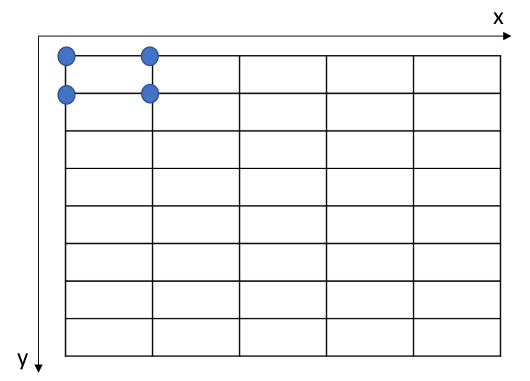
\includegraphics[width=2.5in]{figures/twoagent1.png}
  \caption{Arrangement of agents at the beginning(when $a=2$)}\label{fig:twoagent1}
\end{figure}
Now let's consider the routes for the agents. For convenience, we assume that all the agents move at $T(x)\,(x\in\mathbb{Z}^*)$ because some time should be reserved for the coordination after the BV is triggered. More detail about the moving cycle would be discussed after we decide the number of agents and the routes for them. 
Let $v=(x, y)$ be the node under exploration, with $1\leq x_i \leq d_1$, $1\leq i \leq d_2$. Additionally, we define ``Vertical Moving Mark'' (VMM) for every agent: VMM can only change between $0$ and $1$; every time when the agent moves SOUTH, that value changes. For example, if one agent continues to move SOUTH at $T(x)\,(x\in\mathbb{Z}^*)$ and its $Vertical_D$ is originally $0$, then its $Vertical_D$ changes into $1$ at $T(1)$, $0$ at $T(2)$ and so on.
Every agent hold two VMMs in its memory and let's say $VMM_1$ and $VMM_2$. The original value of $VMM_1$ of the agents is $0$; the original value of $VMM_2$ of agents residing at node $(1, y)$ and node $(2, y)$ ($1\leq y\leq a$) is $0$ and $1$ respectively. 

we now define the action of the $2a\,(a\in\mathbb{Z}^*)$ agents:\\ 
\begin{itemize}
\item Let $b=a-1$. When all agents' $VMM_1$ are ``0", then those agents with $VMM_2$ equal to ``0" move EAST when $x\neq d_1-1$ and move SOUTH for $b$ steps when $x=d_1-1$; those agents with $VMM_2$ equal to ``1" move EAST when $x\neq d_1$ and move SOUTH for $b$ when $x=d_1$. When all agents' $VMM_1$ are ``0", then those agents with $VMM_2$ equal to ``0"  move WEST when $x\neq2$ and move SOUTH for $b$ steps when $x=2$; those agents with $VMM_2$ equal to ``1" move WEST when $x\neq 1$ and move SOUTH for $b$ steps when $x=1$.
\item A agent only move to a node which it has not explored. (Note that when residing at a node, a agent is able to know whether it has explored the neighbours of that node or not.)
\end{itemize}
Informally, the routes of agents are snakelike routes. When $a=2$, the routes of agents are shown as Fig\ref{fig:twoagent2}.
%\iffalse
\begin{figure} [H]
  \centering 
  \subfigure[Routes of agents in the first line when $a=2$]{ 
    \label{fig:agentroute:a} %% label for first subfigure 
    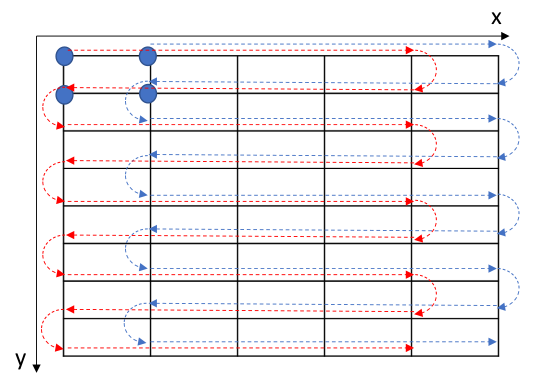
\includegraphics[width=3.5in]{figures/twoagentroute1.png}} 
 \hspace{1in} 
  \subfigure[Routes of agents in the second line when $a=2$]{ 
    \label{fig:agentroute:b} %% label for second subfigure 
    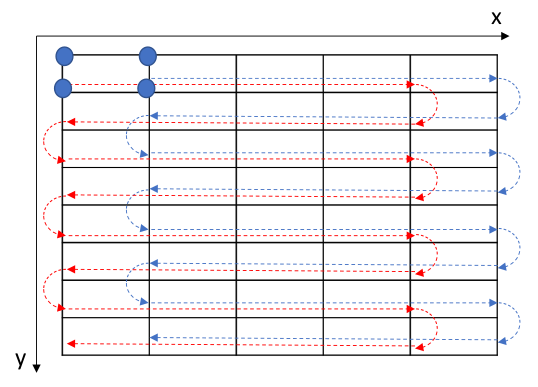
\includegraphics[width=3.5in]{figures/twoagentroute2.png}}
  \caption{Routes of agents when $a=2$} 
  \label{fig:twoagent2} %% label for entire figure 
\end{figure}
%\fi


when $a=3$, the routes of agents are shown as Fig\ref{fig:threeagent1}. 
\begin{figure} [H]
  \centering 
  \subfigure[Routes of agents in the first line when $a=3$]{ 
    \label{fig:agentroute:a} %% label for first subfigure 
    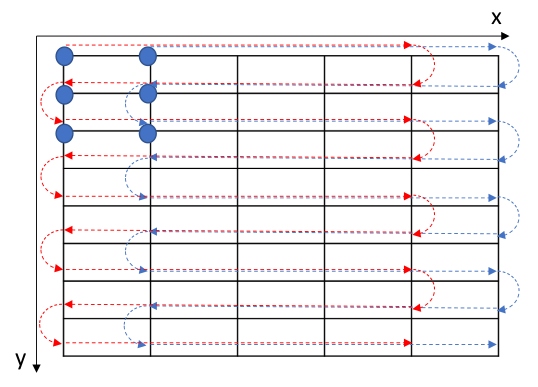
\includegraphics[width=3.5in]{figures/threeagentroute1.png}} 
  \hspace{1in} 
  \subfigure[Routes of agents in the second line when $a=3$]{ 
    \label{fig:agentroute:b} %% label for second subfigure 
    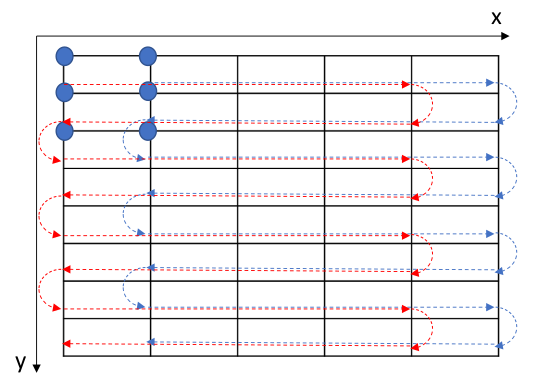
\includegraphics[width=3.5in]{figures/threeagentroute2.png}}
    \hspace{1in} 
    \subfigure[Routes of agents in the second line when $a=3$]{ 
    \label{fig:agentroute:c} %% label for second subfigure 
    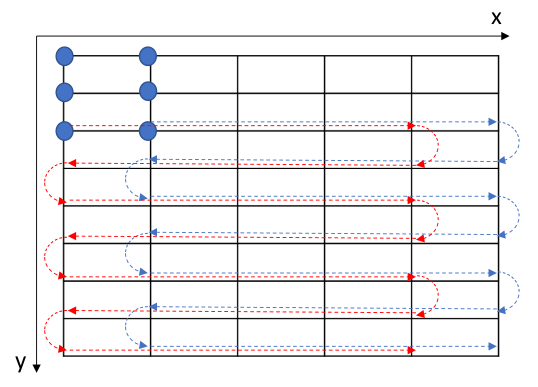
\includegraphics[width=3.5in]{figures/threeagentroute3.png}}
  \caption{Routes of agents when $a=3$} 
  \label{fig:threeagent1} %% label for entire figure 
\end{figure}





Initially, 2$d_1$ agents are placed at the first two columns at $T_0$. More specifically, the coordinate of them are (1, $x_i$) and (2,$x_i$) where $1\leq x_i\leq d_1$. The agents residing in the first column are in the shadowing group while the agents residing in the second column are in the exploring group. If the BV resides in a node in the first column, then all of its clones are destroyed. If the BV resides in a node in the second column, then the elimination phase begins. It is obvious that if the BV do not reside in any node in the first column, then a agent in the exploring group should be destroyed when the BV is exposed.  Let's assume that the we starts at $T_0$. Agents residing in nodes in the second column moves EAST at the beginning of T(2n), $n=0,1, \ldots ,d_2-1$. More precisely, node (x, y) move to (x+1, y) at the beginning of T(2n), $n=0,1, \dots , d_2-1$. Agents residing in the first column simply follow the node in the second column (see  Fig.\ref{fig:TShE}). When one of the node in the former column is destroyed by a BV, the second phase starts.
\begin{figure}[H]
  \centering  
  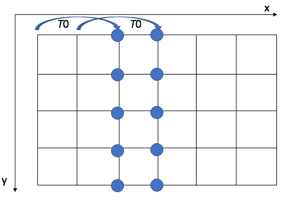
\includegraphics[width=2.5in]{figures/TShE.png}
  \caption{Agents move at time $T_0$}\label{fig:TShE}
\end{figure}
\noindent{\bf Elimination Phase}\\
The elimination begins when one of the node in the former column is destroyed by a BV( let's say, at T(2$x_i$)). No matter where is the BV, there are always three agents residing on its north(if the BV is not in the first line), west and south (if the BV is not in the last line), so only one BV clone survives. In another word, only one node becomes BV node after the BV being triggered.  Observe that in the parallel strategy, not all agents participate in the elimination phase automatically when the BV is explored because only those receive the clones of the original BV and those be notified by other agents can participate in the elimination phase. Since we want to make use of the agents we employ at the beginning in the elimination phase which means the situation that the number of agents is not enough for completing the elimination phase but there are still some agents keeping exploring the graph is not allowed to happen. So in some situation, agents who receive the BV clone should notify other agents to participate in the elimination.  Let the node where the surviving clone resided be $(x, y)$ and its situation can be divided into four cases. Different routes of agents in the elimination phase are based on the location of the new formed BV.
\begin{itemize}
\item Case 1: When $2<x<d_1$, $1<y<d_2-1$ (a interior node becomes a new formed BV), then agents (let's say agents $a,b,c$) residing in node $(x-1, y+1)$, $(x-1, y-1)$ and $(x-2, y)$ receive a BV clone at T(2$x_i$+1), so that they know the location of the original BV and also the new formed BV. Note that in the exploring phase, the agents move EAST at T(2n), $n=0,1, \ldots ,d_2-2$. Actually, one unit of time is reserved for some agents to receive the BV clone. After they receive the BV clone, these agents move EAST for one step (for example, to node $(x, y+1)$, $(x, y-1)$ and $(x-1, y)$ and stop. Note that other agents including agents residing in node $(x-2, y+1)$ and $(x-2, y-1)$ (let's say agent d and e) at T(2$x_i$) do not know the existence of the BV so they keep moving EAST. These two agents arrive at nodes $(x, y+1)$, $(x, y-1)$ at T(2($x_i+2$)) and at this time they meet agent $a$ and $b$ respectively. Agent $a$ and $b$ inform them of the location of the new form BV and the routes of agents $d$ and $e$ are as follow:\\
route of $d$: $(x, y+1)(at\ T(2(x_i+2)){\rightarrow}(x+1,y+1)(at\ T(2(x_i+2)+1){\rightarrow}(x+1,y)(at\ T(2(x_i+3))$.\\
route of $e$: $(x, y-1)(at\ T(2(x_i+2)){\rightarrow}(x, y)(at\ T(2(x_i+3)+1))$.
The routes of agents are showed in Fig.\ref{fig:subfigmesh1} where a blue node indicate that there are one agent residing here; a red node indicate that there are two agents residing here; a yellow node indicate that there are three agents residing here.

%\iffalse
\begin{figure} [H]
  \centering 
  \subfigure[$T(2x_i+1)$]{ 
    \label{fig:subfigmesh1:a} %% label for first subfigure 
    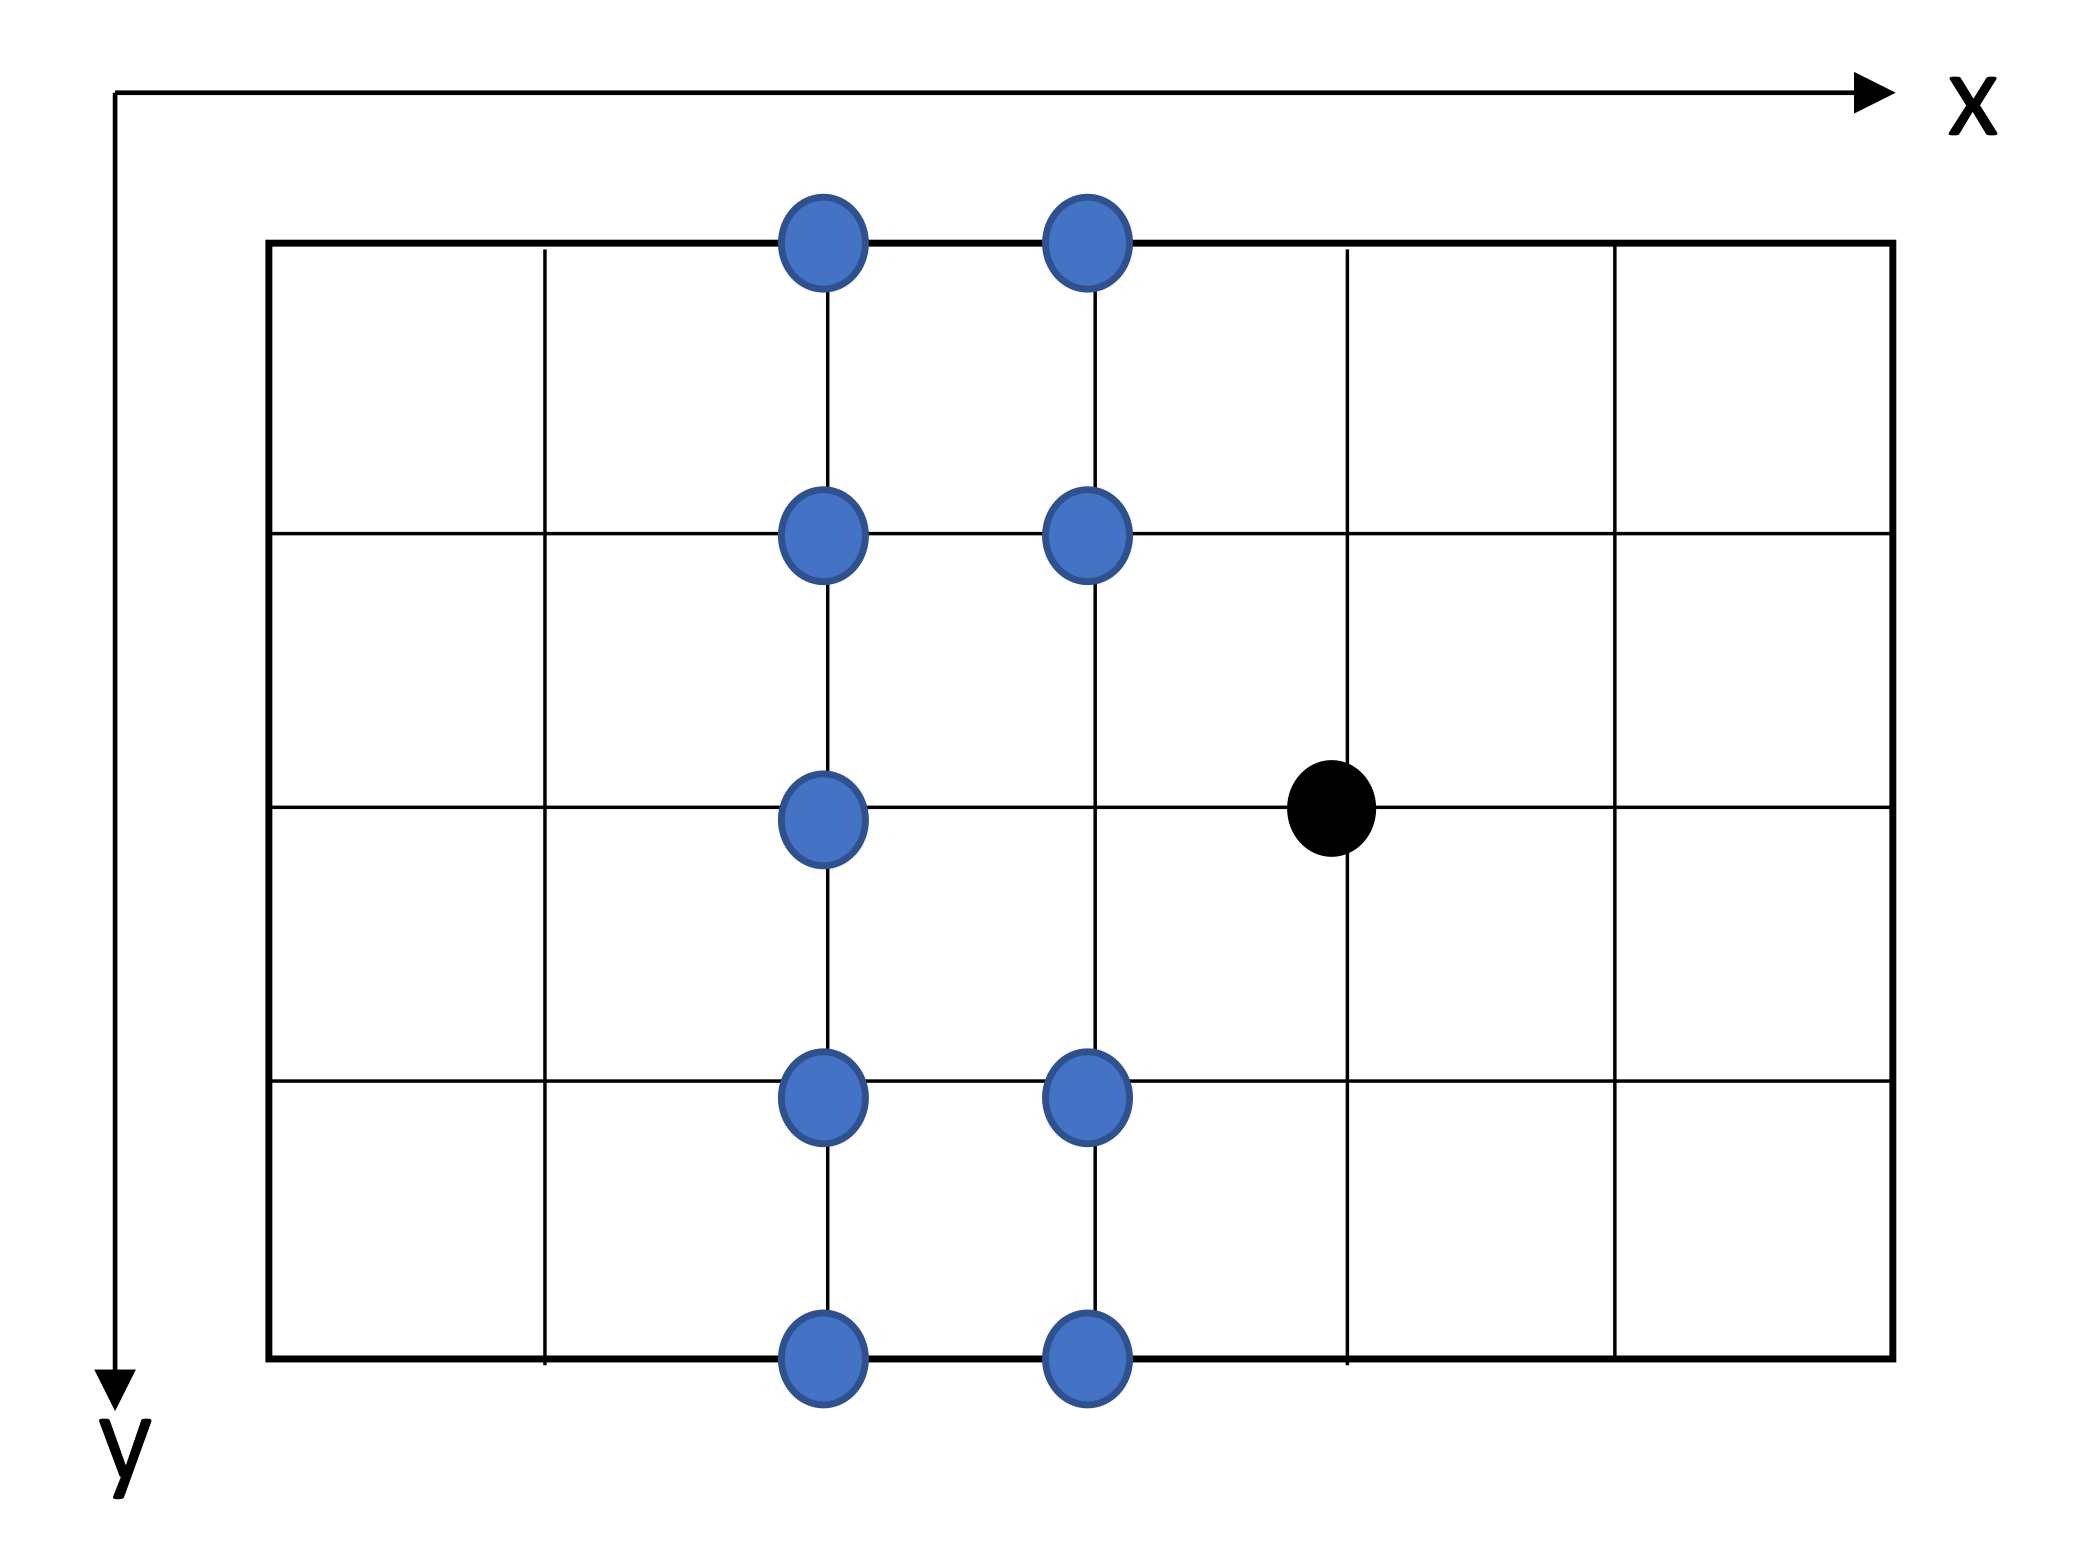
\includegraphics[width=2.5in]{figures/meshinterior.png}} 
%  \hspace{1in} 
  \subfigure[$T(2(x_i+1))$]{ 
    \label{fig:subfigmesh1:b} %% label for second subfigure 
    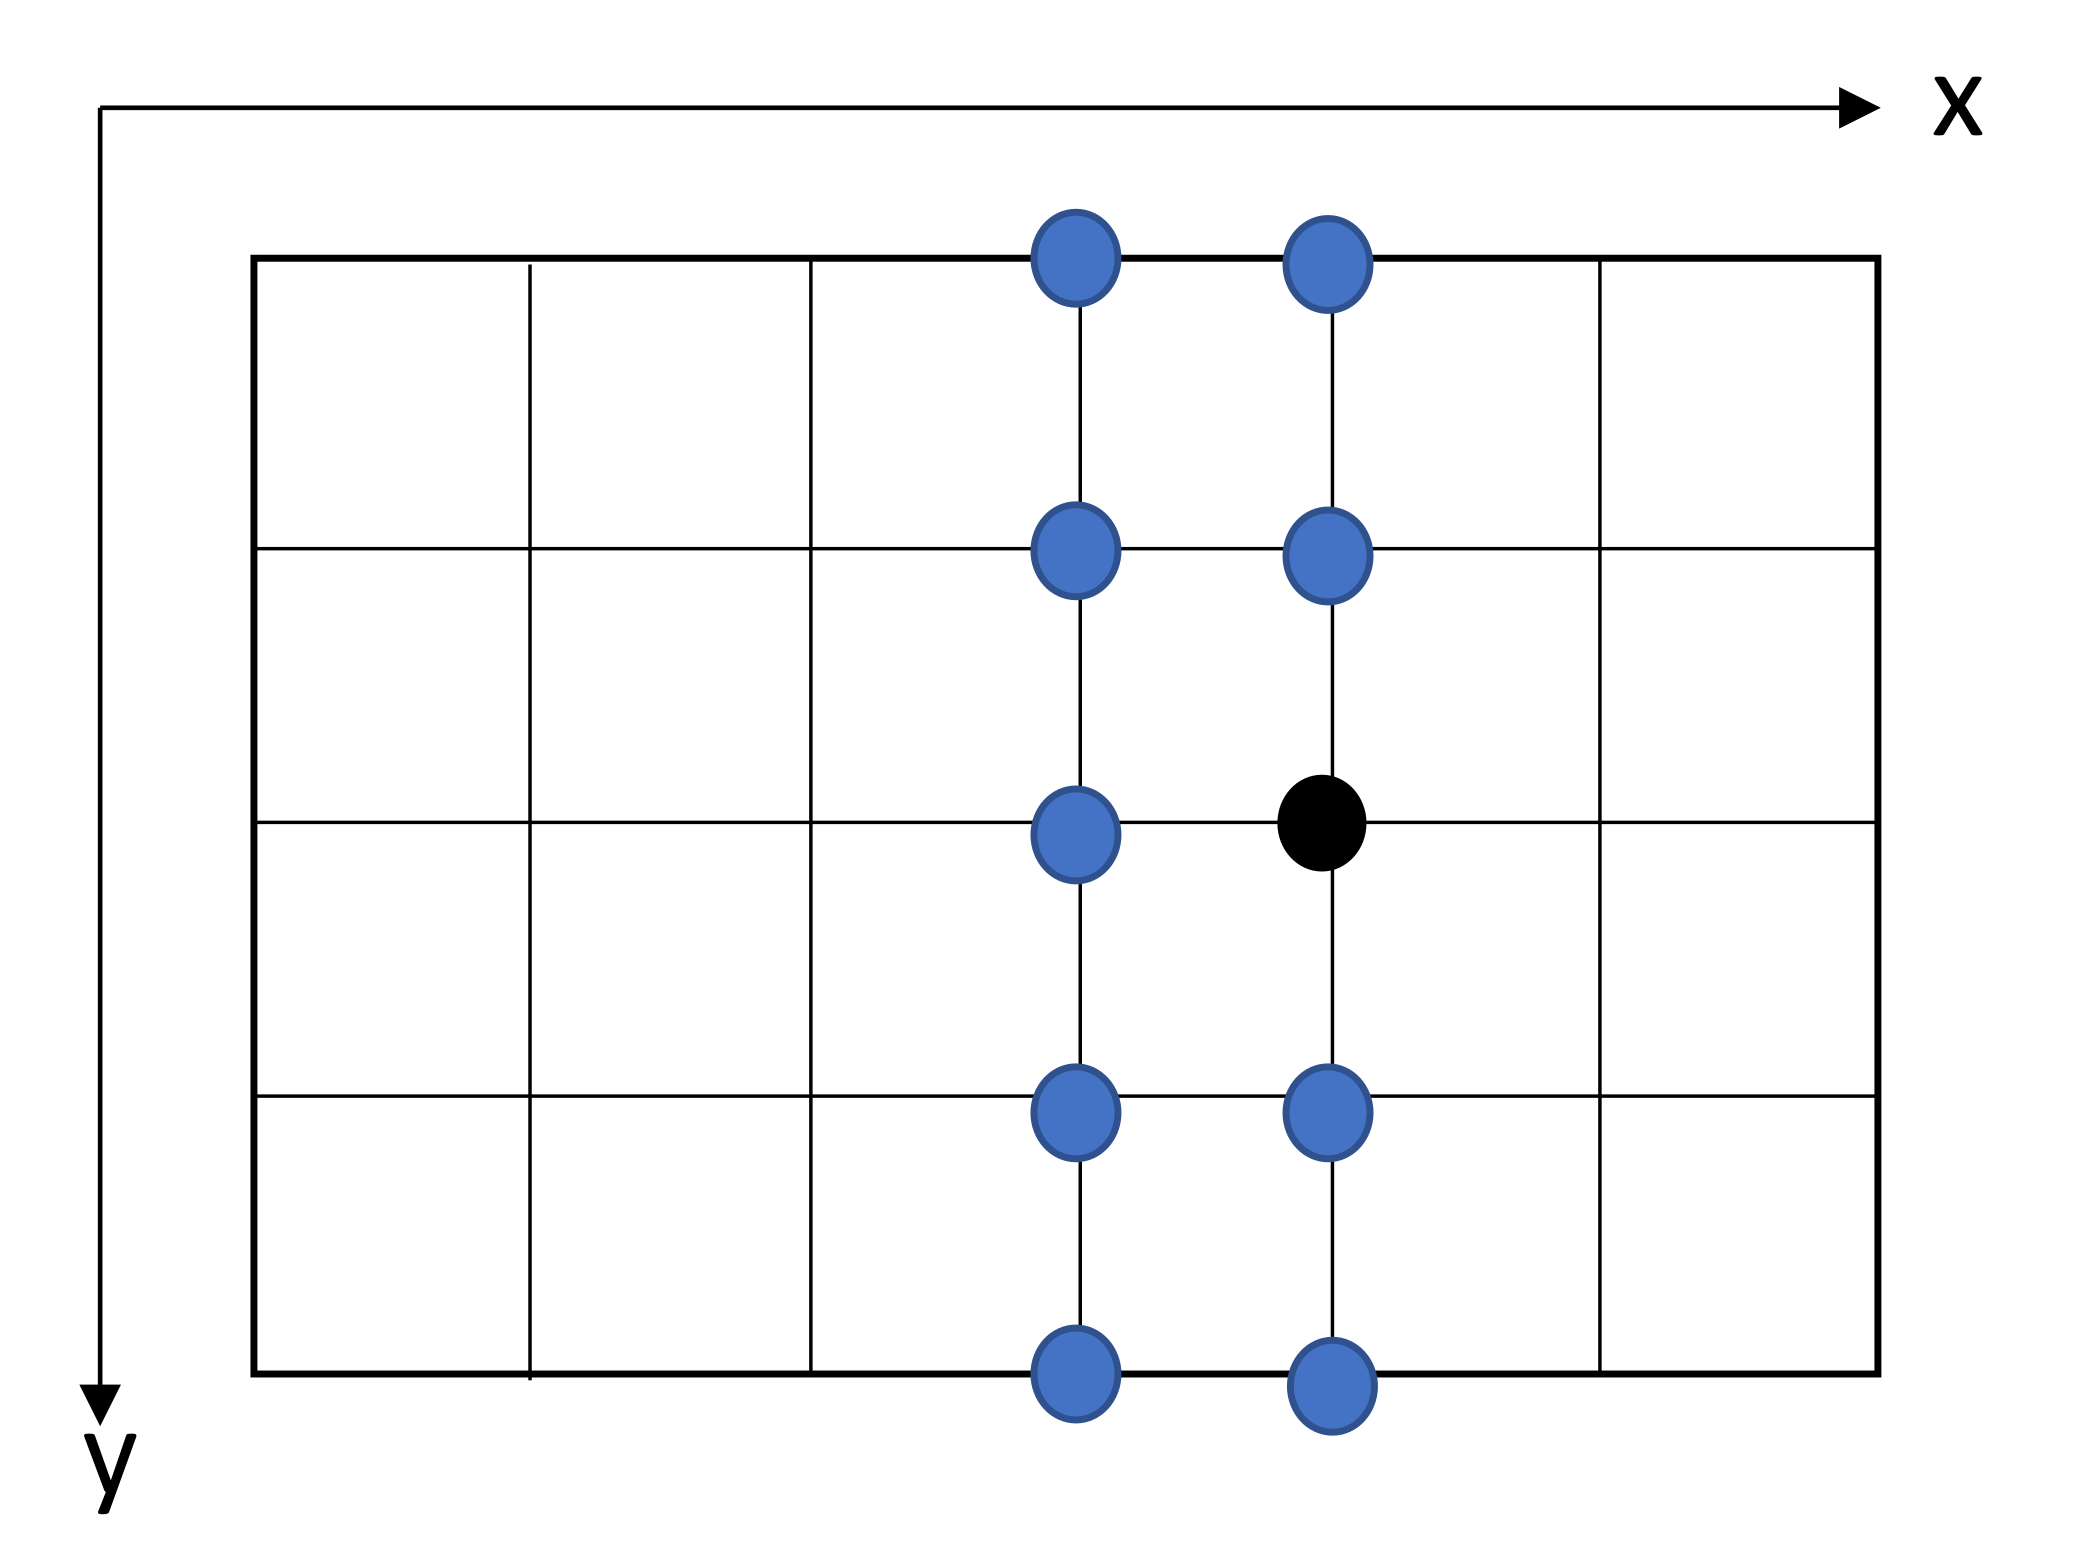
\includegraphics[width=2.5in]{figures/meshinterior1.png}}
    \hspace{1in} 
  \subfigure[$T(2(x_i+2))$]{ 
    \label{fig:subfigmesh1:c} %% label for second subfigure 
    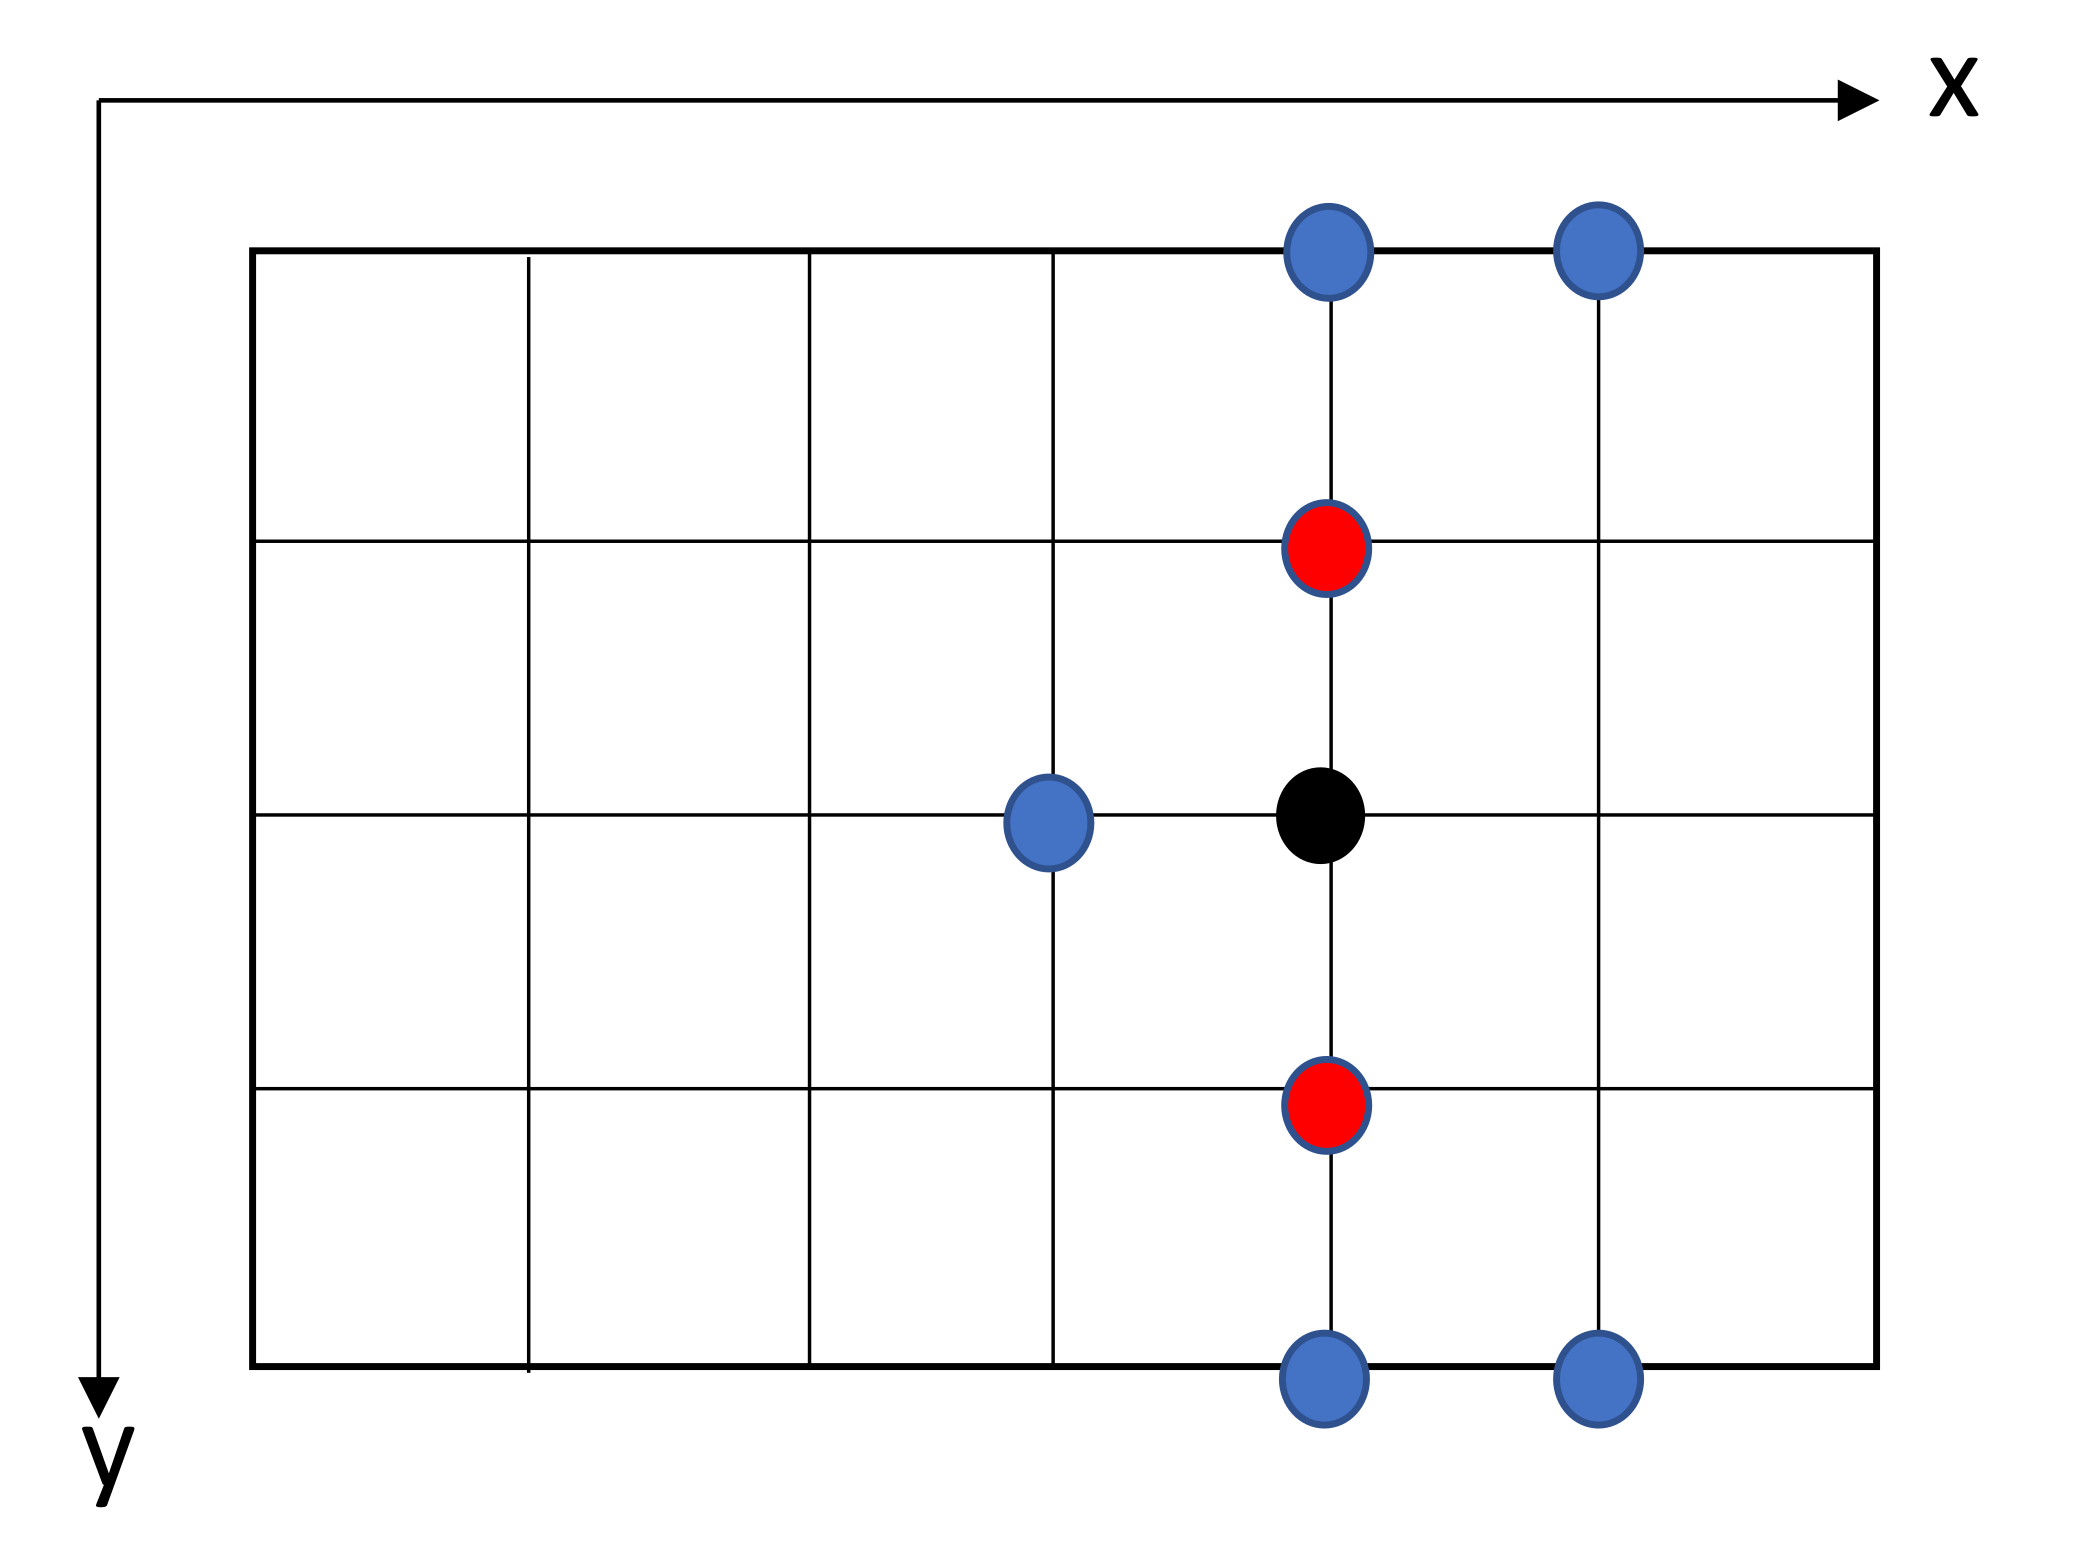
\includegraphics[width=2.5in]{figures/meshinterior2.png}}
%      \hspace{1in} 
  \subfigure[$T(2(x_i+3))$]{ 
    \label{fig:subfigmesh1:d} %% label for second subfigure 
    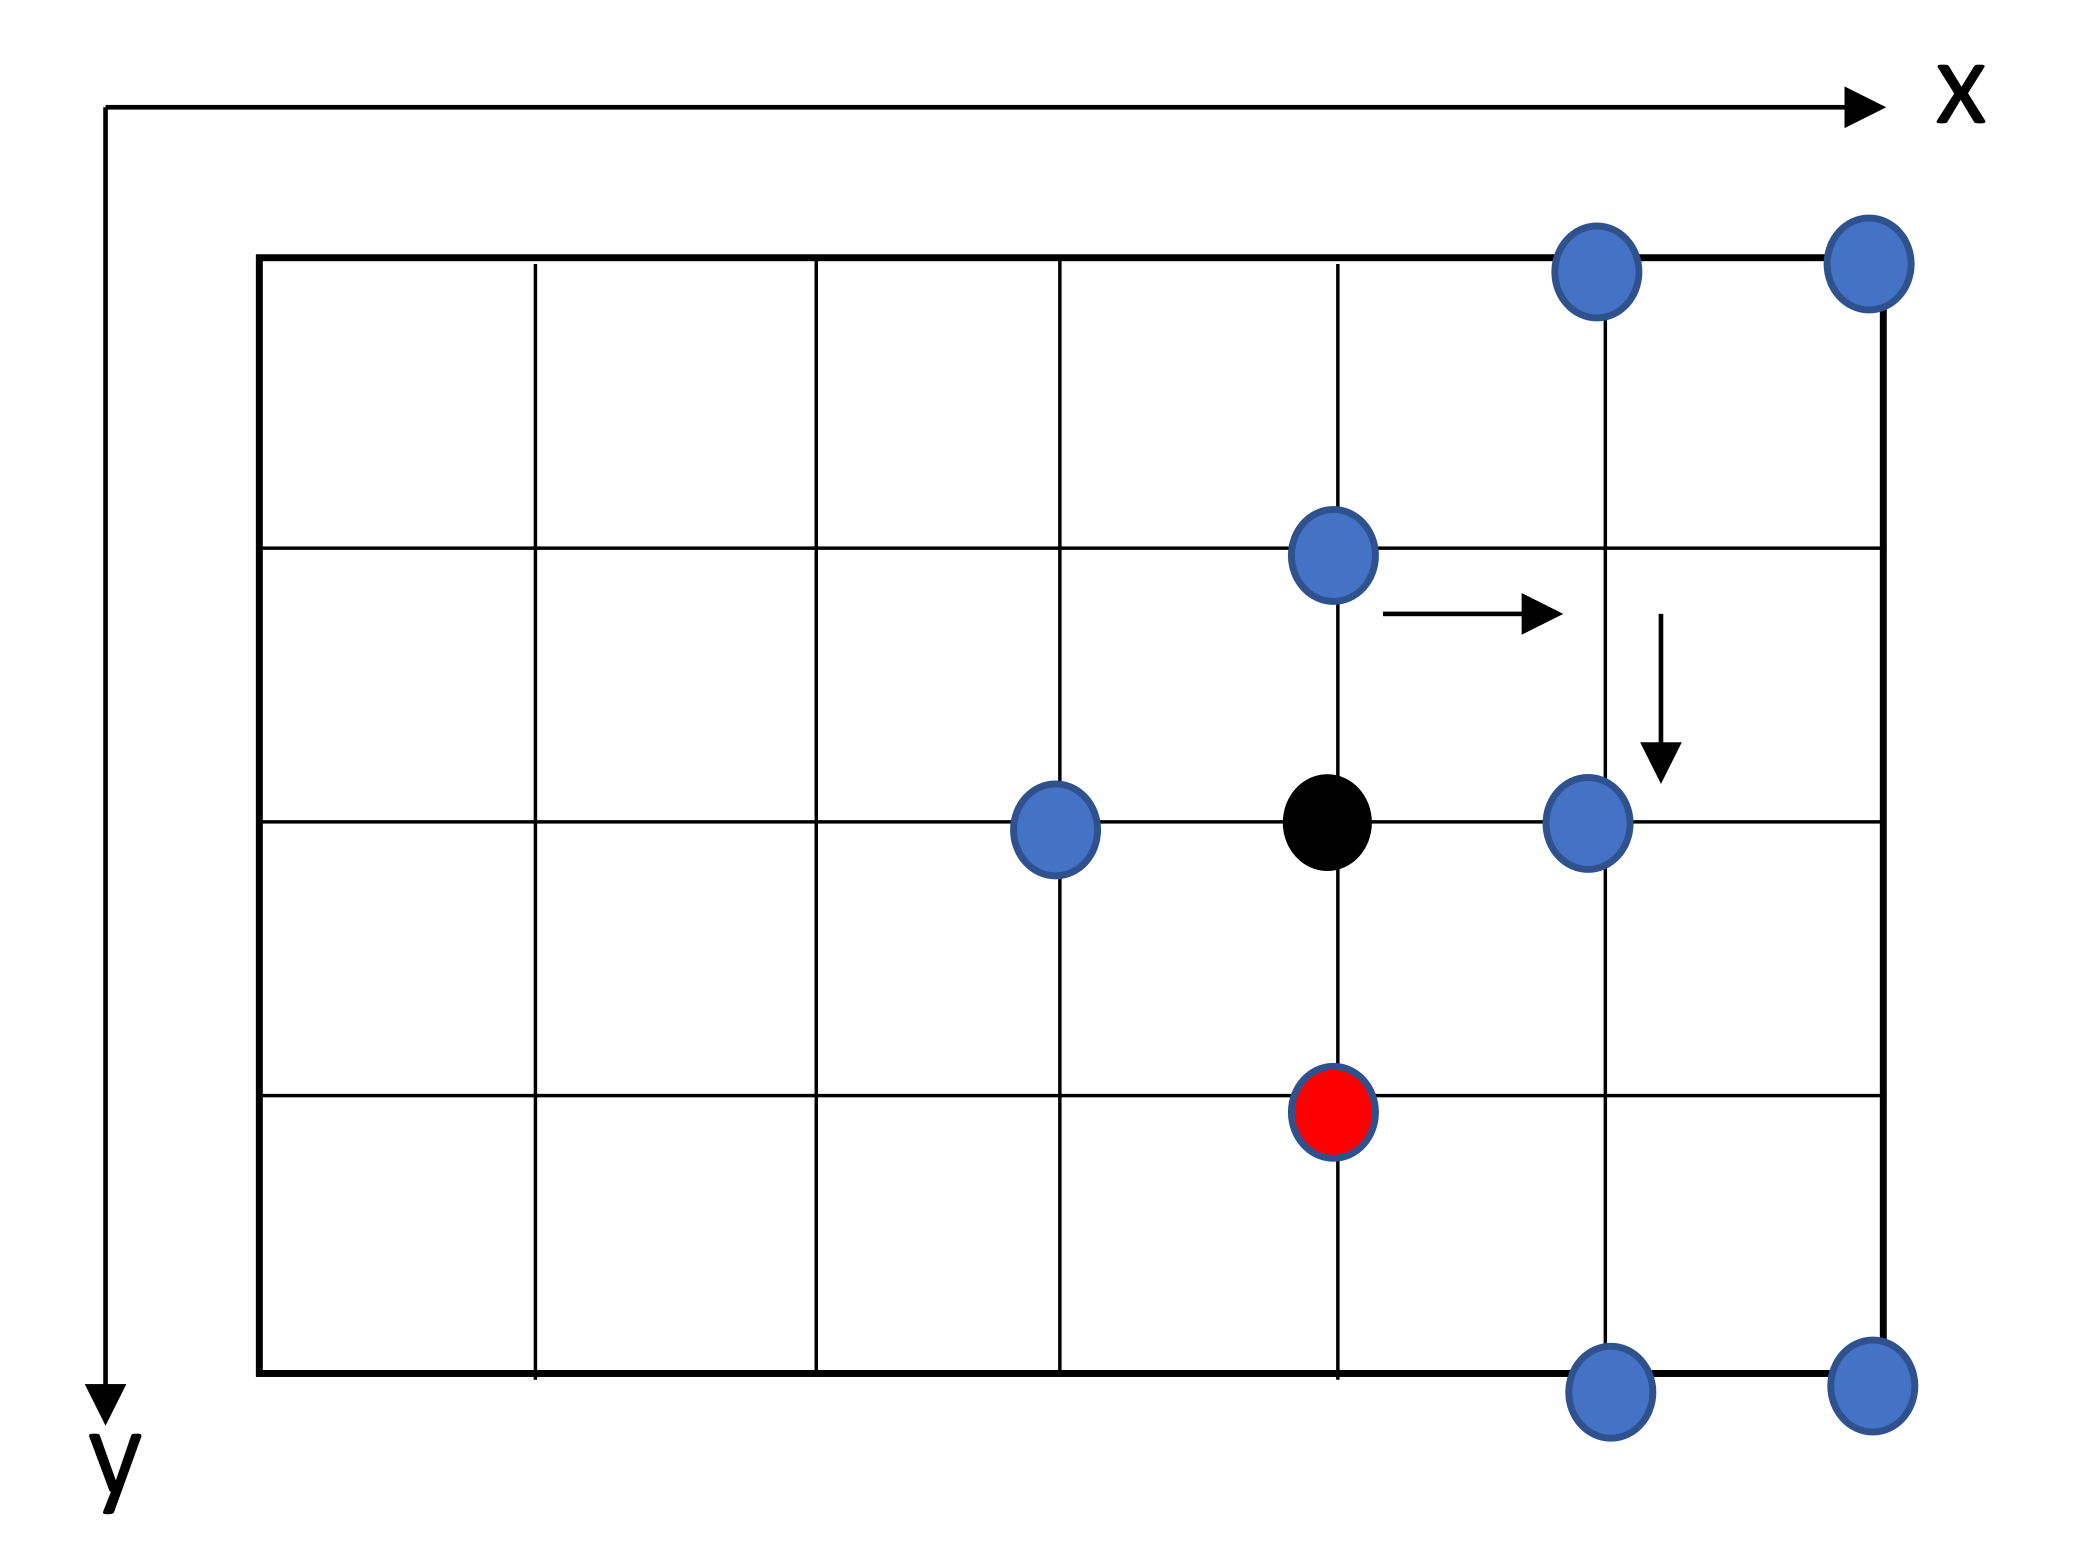
\includegraphics[width=2.5in]{figures/meshinterior3.png}}
      \hspace{1in} 
  \subfigure[$T(2(x_i+3)+1)$]{ 
    \label{fig:subfigmesh1:e} %% label for second subfigure 
    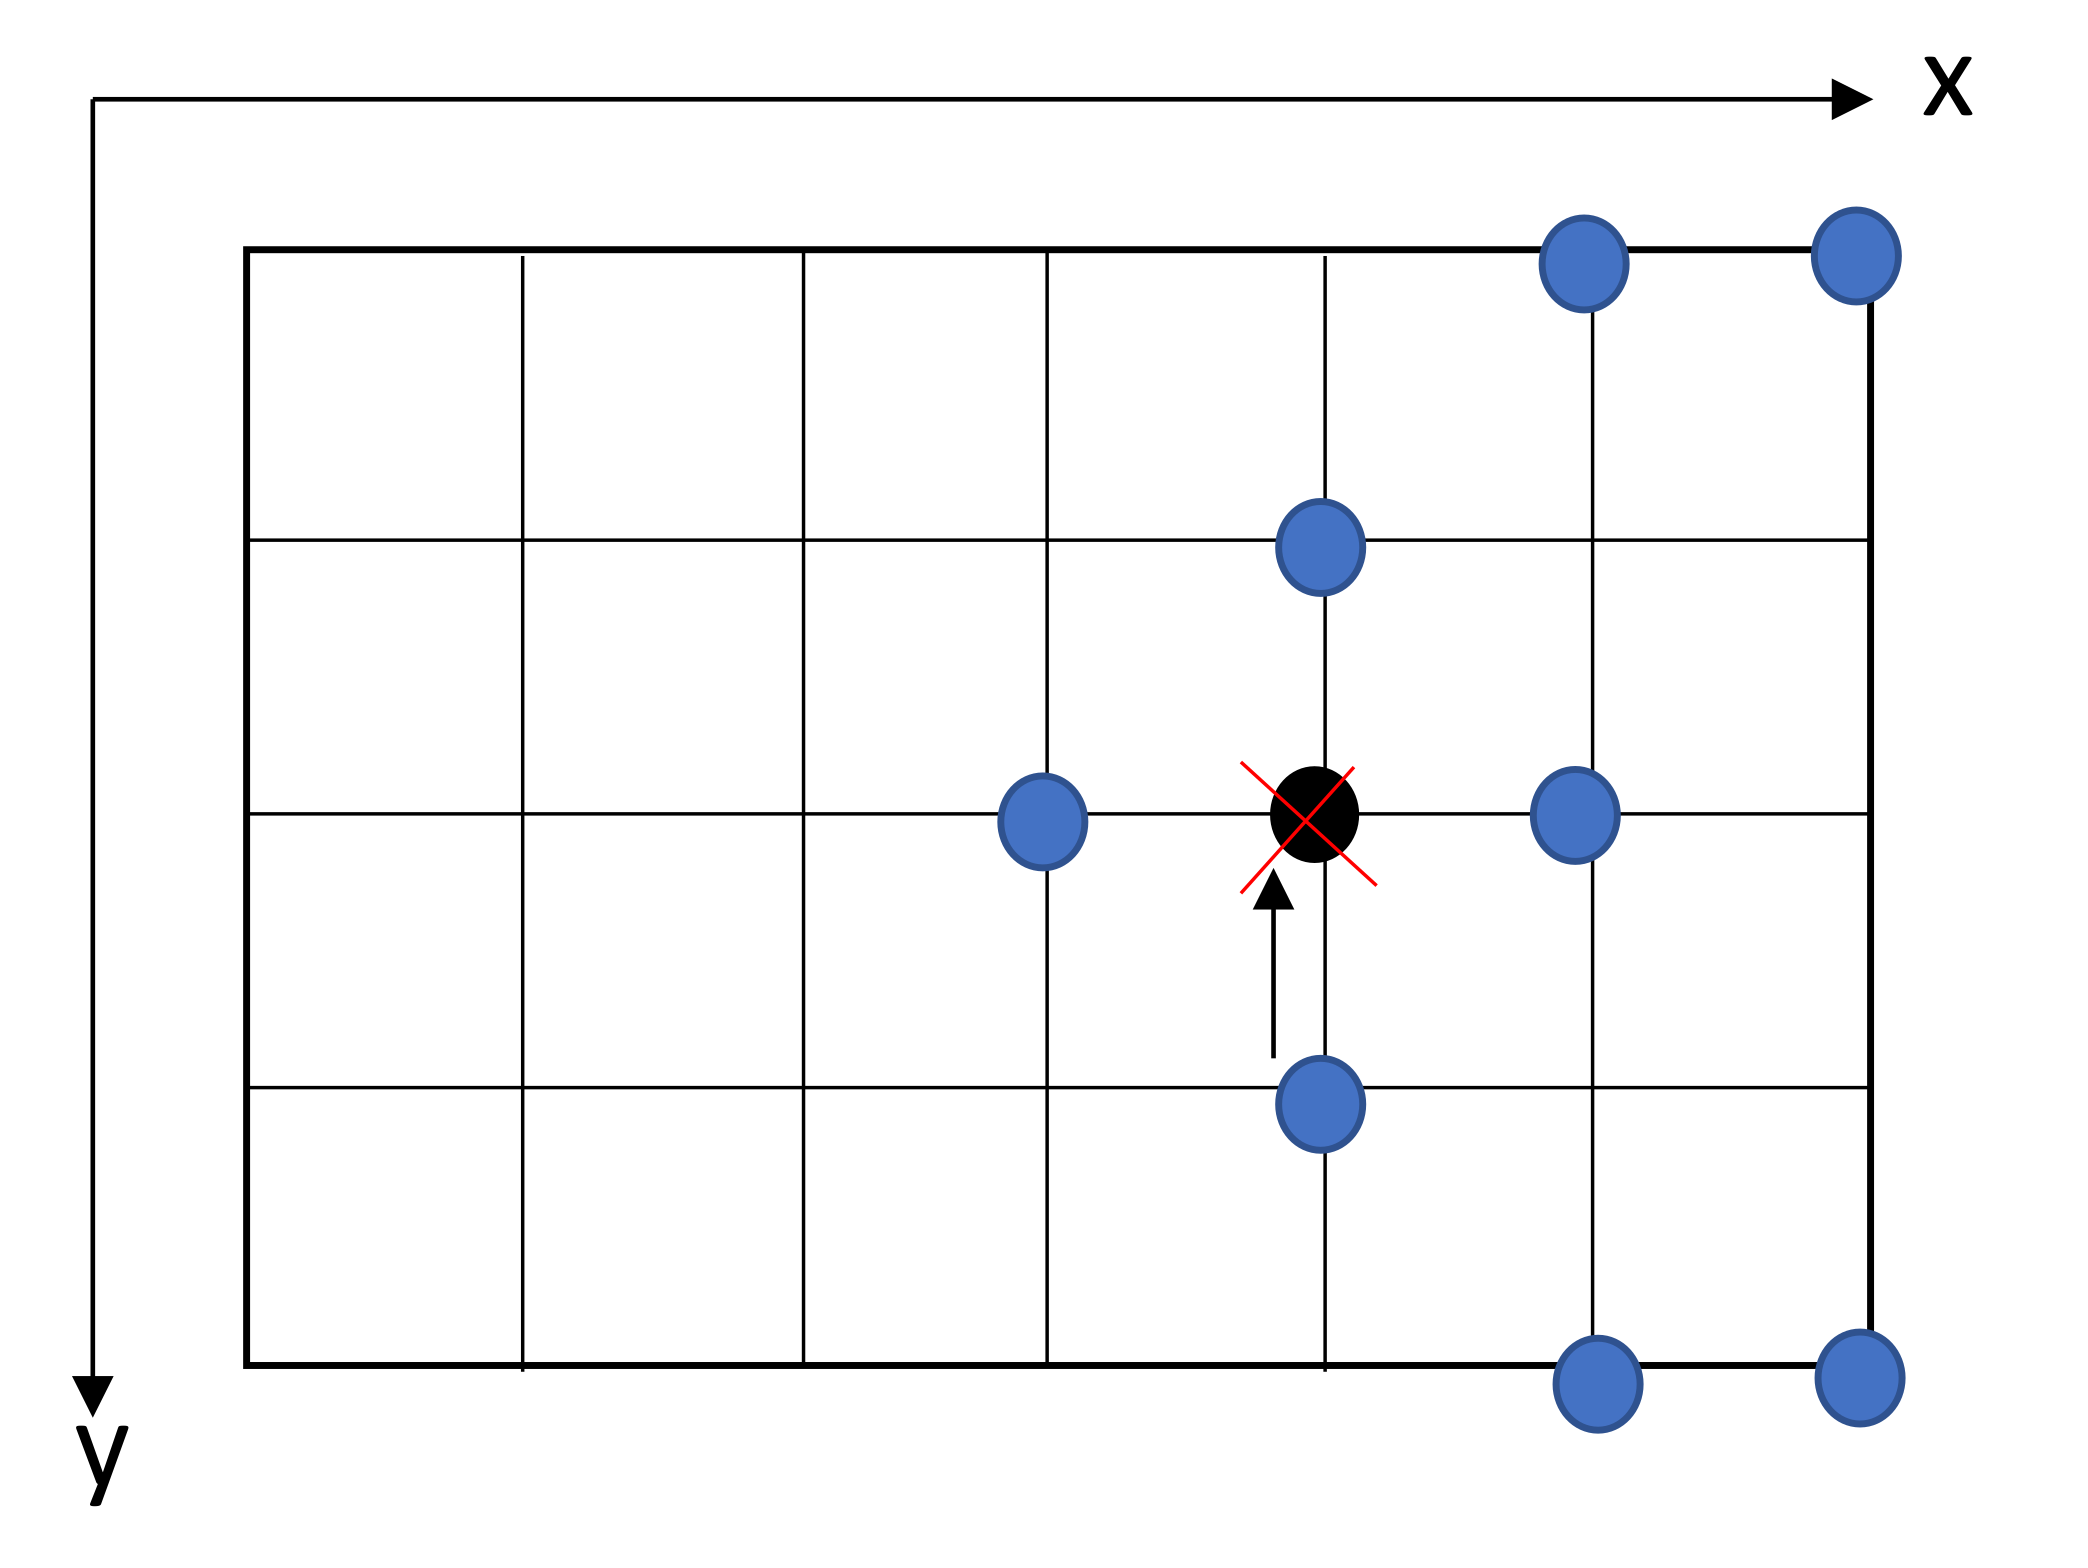
\includegraphics[width=2.5in]{figures/meshinterior4.png}}
  \caption{Arrangement of agents in elimination phase when the new formed BV resides in a interior node} 
  \label{fig:subfigmesh1} %% label for entire figure 
\end{figure}
%\fi


\item Case 2: When $x=d_1$, $2<y<d_2-1$ (a border node becomes a new formed BV), then agents (let's say agents $a,b,c$) residing in node $(x-1, y+1)$, $(x-1, y-1)$ and $(x-2, y)$ receive a BV clone at T(2$x_i$+1). As above, they move EAST for one step and stop. Agents residing in nodes $(x-2, y+1)$ and $(x-2, y-1)$ (let's say agents $a,b$) at T(2$x_i$) have no knowledge of the BV, so they keep moving and arrive at nodes $(x, y+1)$ and $(x, y-1)$ at T(2($x_i$+2)) when they are informed of the location of the new formed BV. One of agents $a$ and $b$ should move to the new formed BV to decontaminate it while the other one stop moving. In order to avoid conflict, we always employ the agent $a$ to move to the new formed BV.
\begin{figure} [H]
  \centering 
  \subfigure[$T(2x_i+1)$]{ 
    \label{fig:subfigmesh2:a} %% label for first subfigure 
    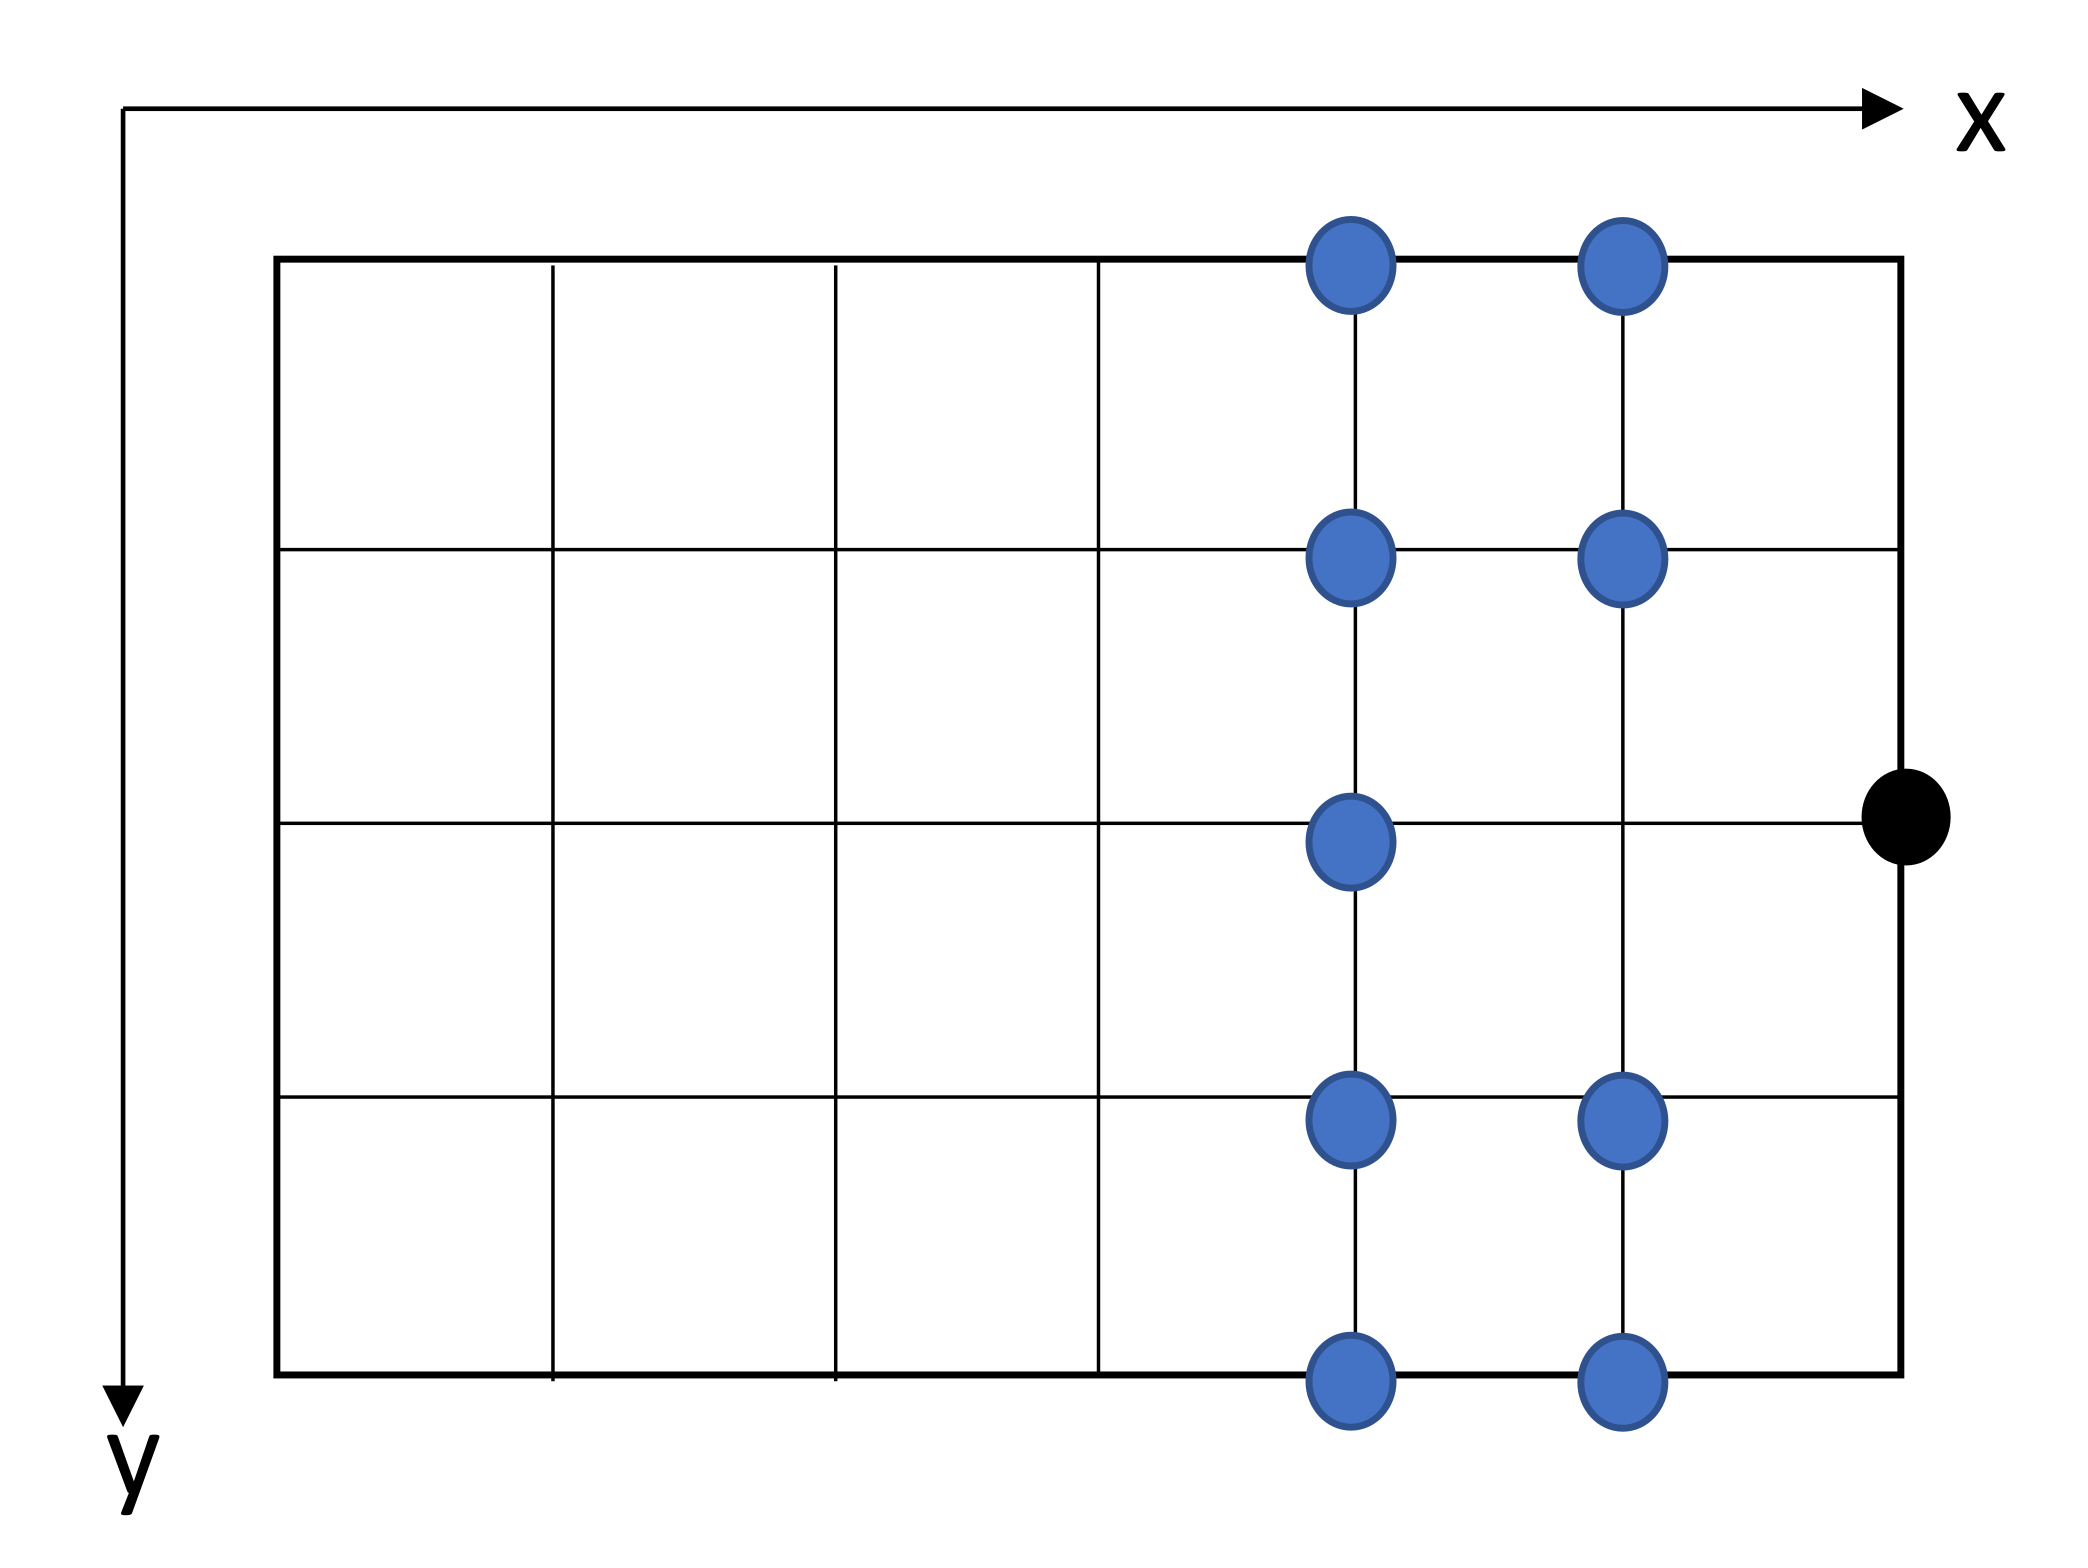
\includegraphics[width=2.5in]{figures/meshborderx1.png}} 
%  \hspace{1in} 
  \subfigure[$T(2(x_i+2))$]{ 
    \label{fig:subfigmesh2:b} %% label for second subfigure 
    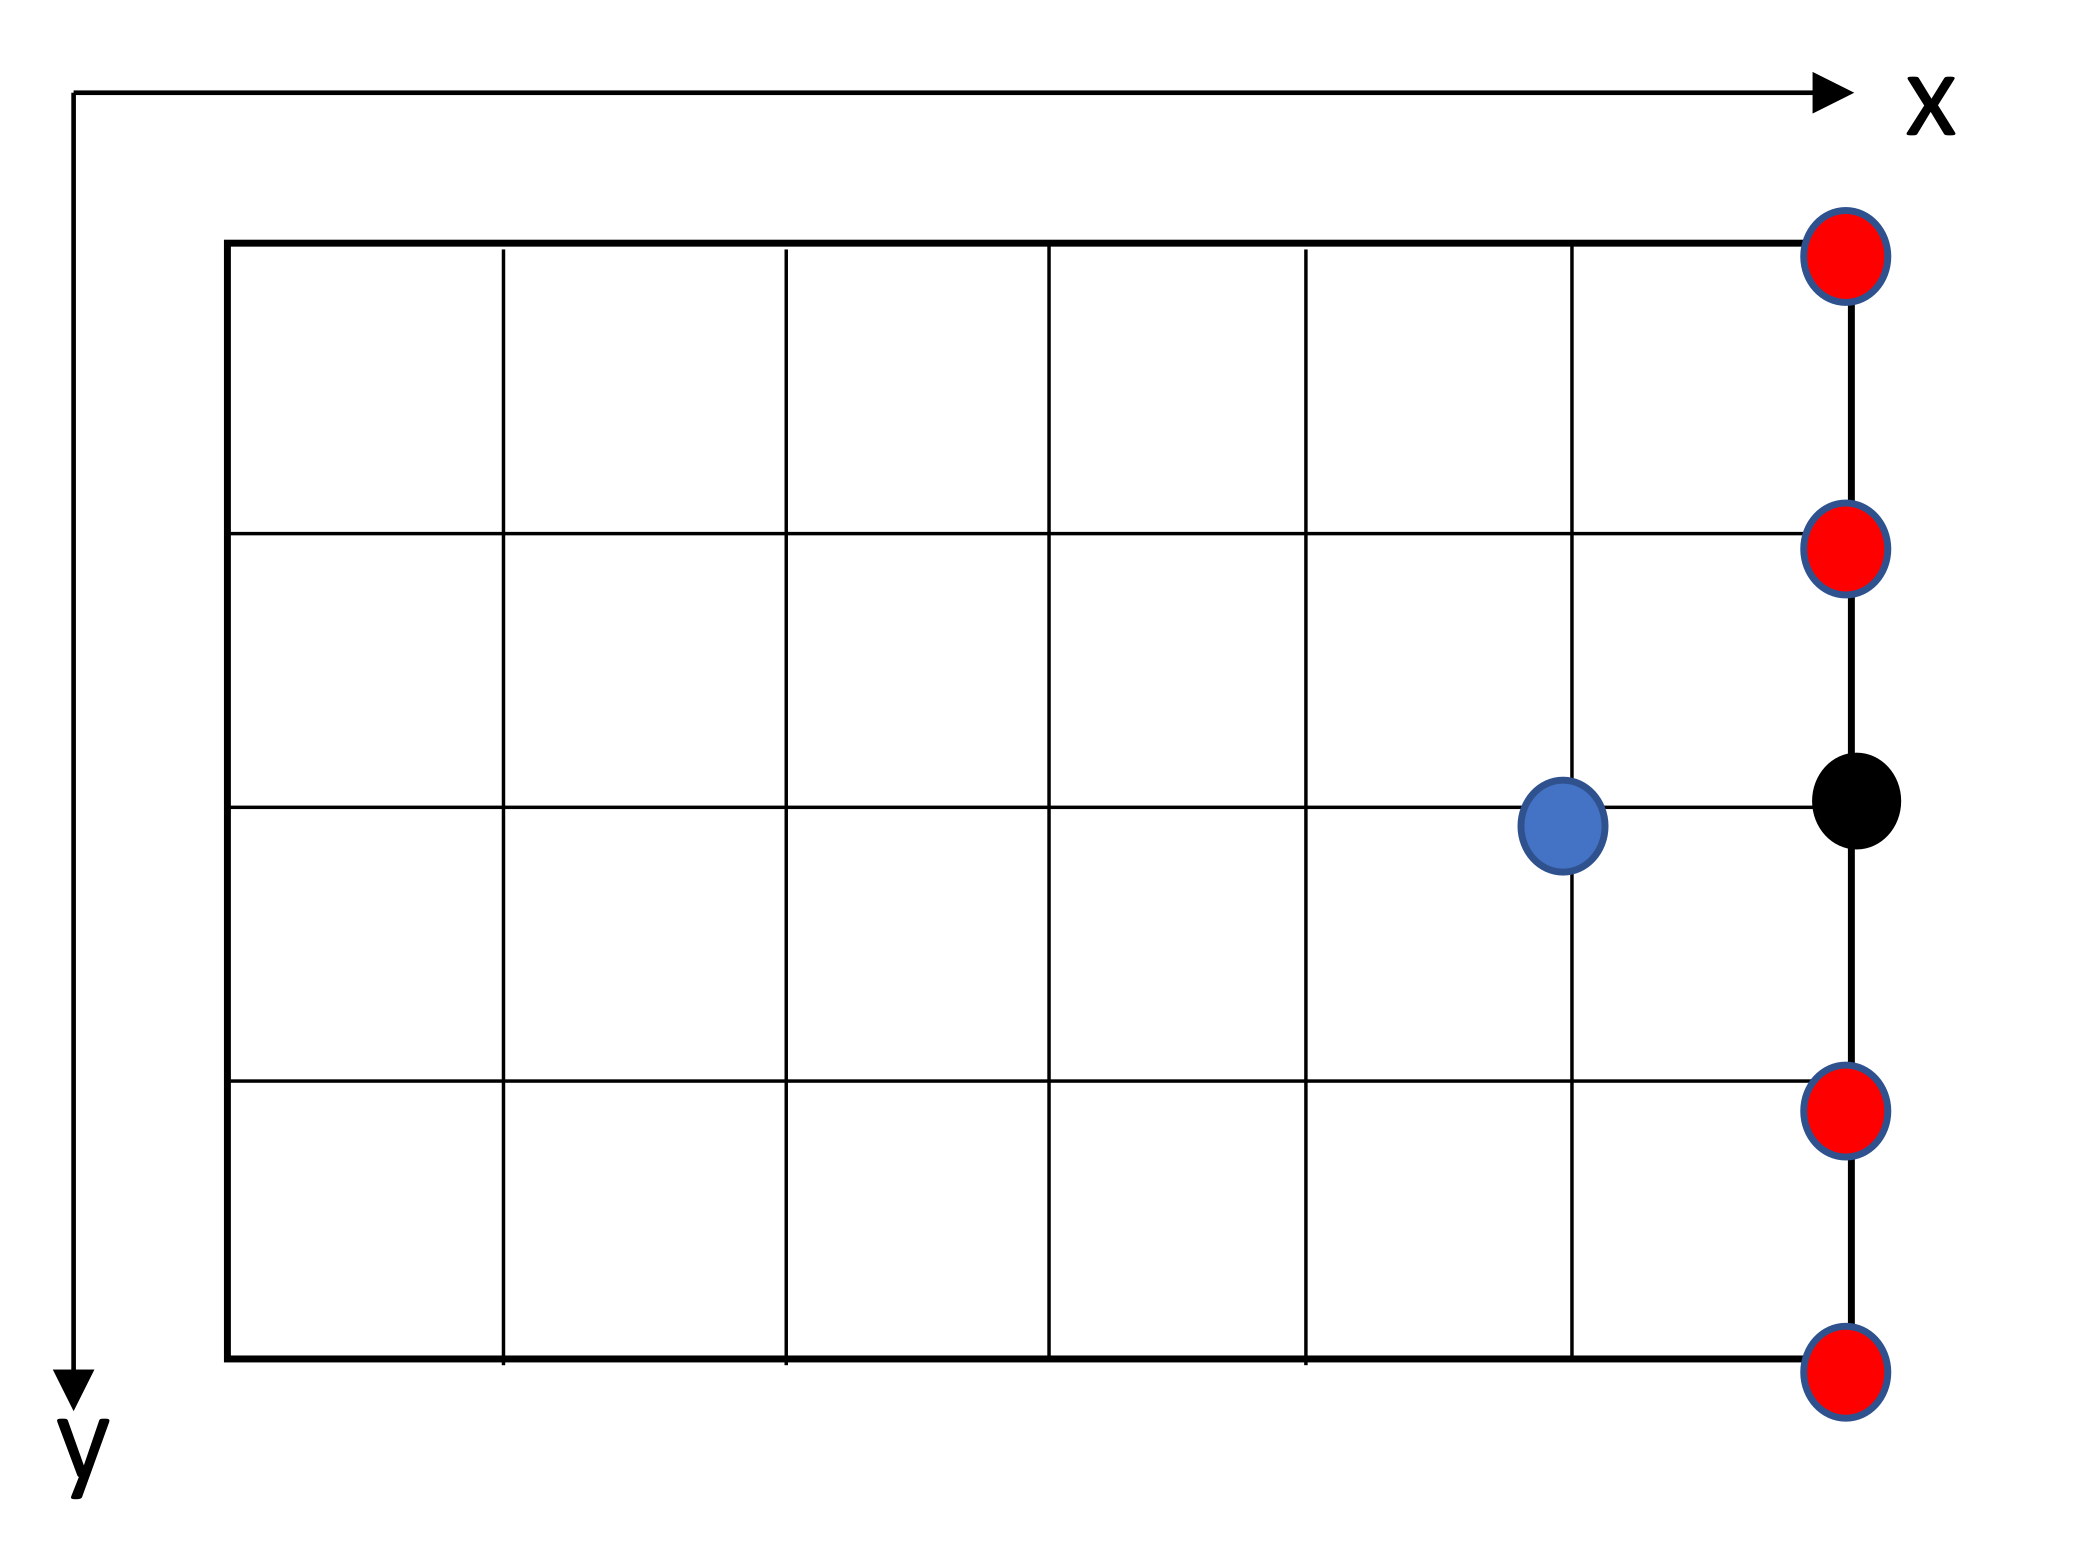
\includegraphics[width=2.5in]{figures/meshborderx2.png}}
    \hspace{1in} 
  \subfigure[$T(2(x_i+2)+1)$]{ 
    \label{fig:subfigmesh2:c} %% label for second subfigure 
    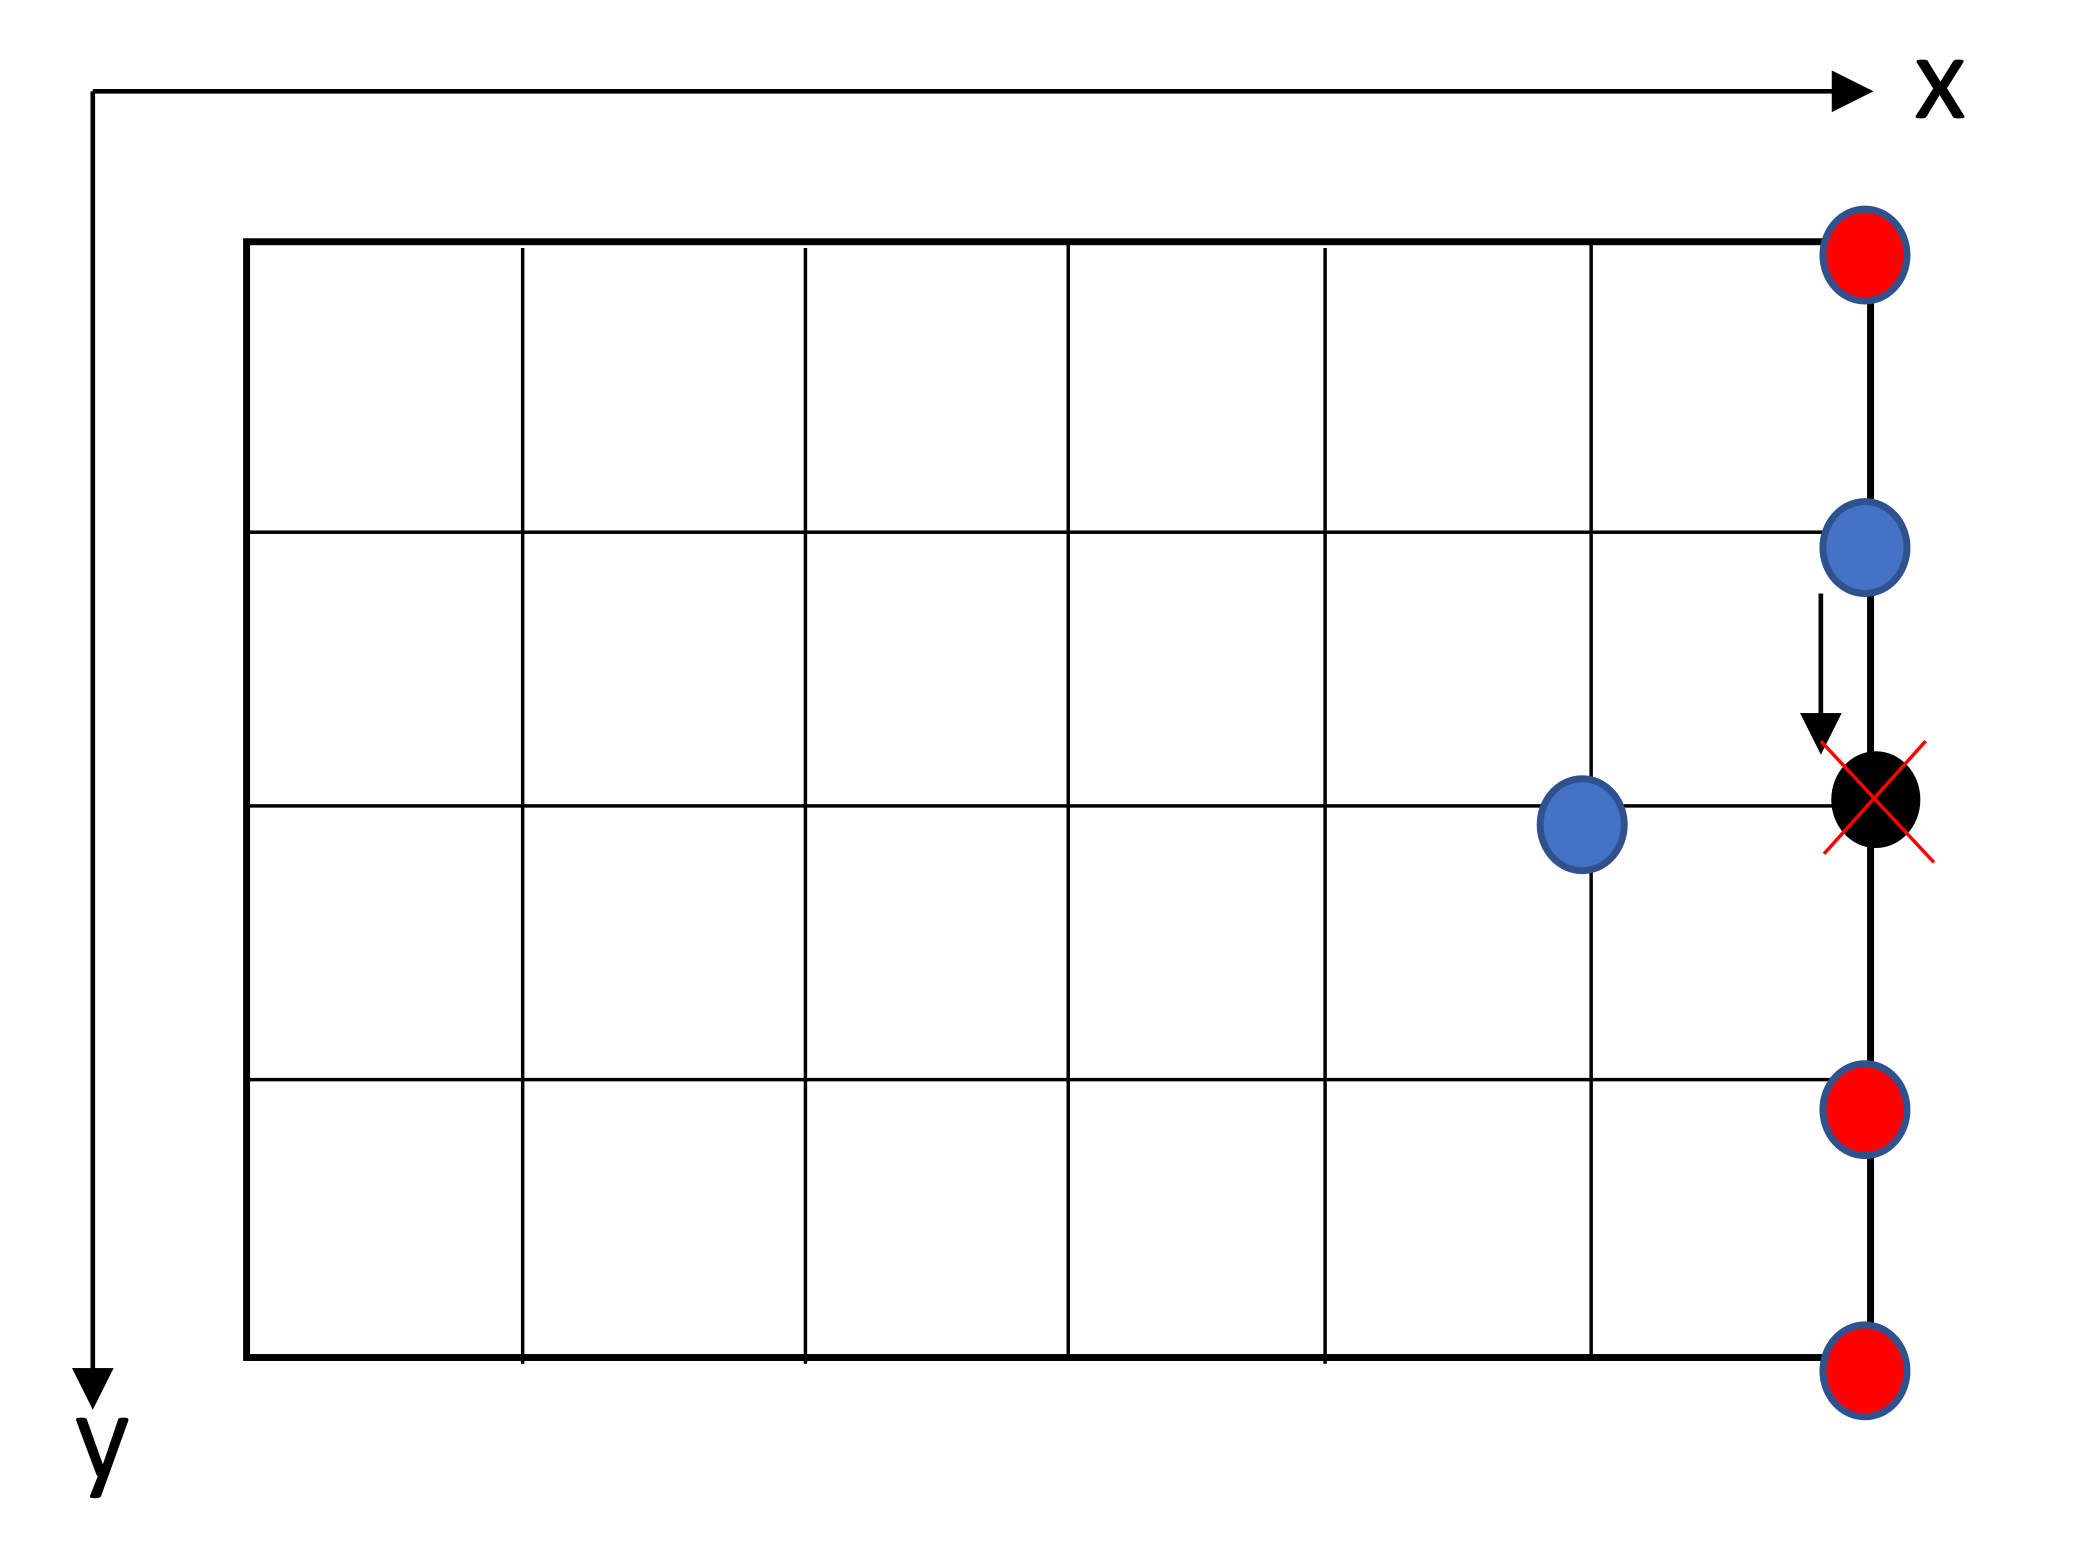
\includegraphics[width=2.5in]{figures/meshborderx3.png}}
%      \hspace{1in} 
    \caption{Arrangement of agents in elimination phase when the new formed BV resides in a border node (when $x=d_1$)} 
  \label{fig:subfigmesh2} %% label for entire figure 
\end{figure}

\item Case 3: When $2<x<d_1$, $y=1$ or $y=d_2-1$ (a border node becomes a new formed BV). For convenience, we only discuss the situation when $y=1$(the solution can be easily modified to fit the scenario when $y=d_2-1$). In this case, agents residing in nodes $(x-1, y+1)$ and $(x-2, y)$ (let's say agents a,b) receive a BV clone at T(2$x_i$+1). Agents $a$ and $b$ move EAST for one step and arrive at node $(x, y+1)$ and node $(x-1, y)$ at T($2(x_i+1)$). Since the number of agents who can be informed of the location of the new formed BV is not enough for decontaminating the BV, we should notify one more agent to participate in the elimination phase. We employ agent $a$ who resides in node $(x, y+1)$ at T(2$x_i$+1) to notify agent residing in node $(x, y+1)$ (let's say agent $c$), so it move NORTH for one step and arrive at node $(x, y+2)$ at T($2(x_i+1)+1$). Then both of agents $a$ and $c$ move SOUTH and reach node $(x, y+1)$ at T($2(x_i+2)$) when the they meet the agent who move from node $(x-1, y+1)$ (let's say agent $d$) and notify it to stop moving. Then agent $a$ move EAST and then SOUTH to reach node $(x+1, y)$ at T($2(x_i+3)$). Finally, at T($2(x_i+3)+1$), agent $d$ move SOUTH to permanently eliminate the BV.

\begin{figure} [H]
  \centering 
  \subfigure[$T(2x_i+1)$]{ 
    \label{fig:subfigmesh3:a} %% label for first subfigure 
    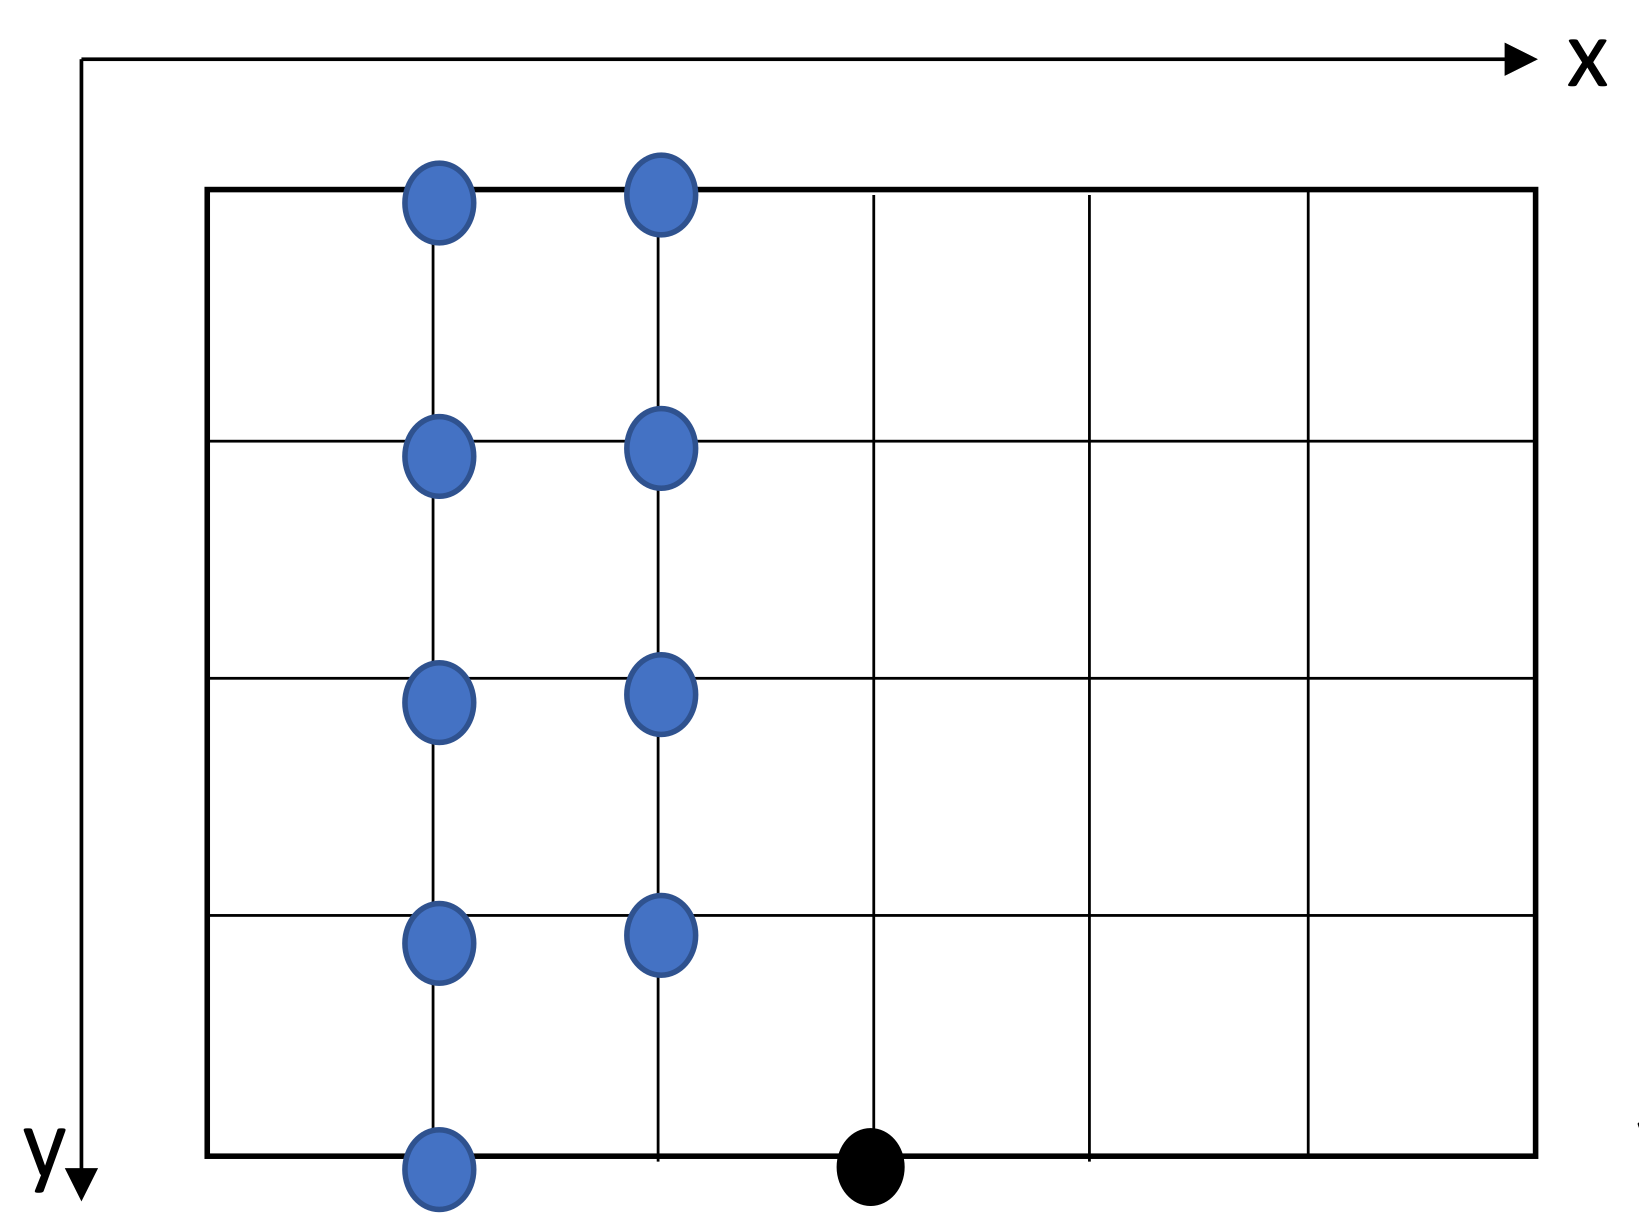
\includegraphics[width=2.5in]{figures/meshbordery1.png}} 
%  \hspace{1in} 
  \subfigure[$T(2(x_i+1))$]{ 
    \label{fig:subfigmesh3:b} %% label for second subfigure 
    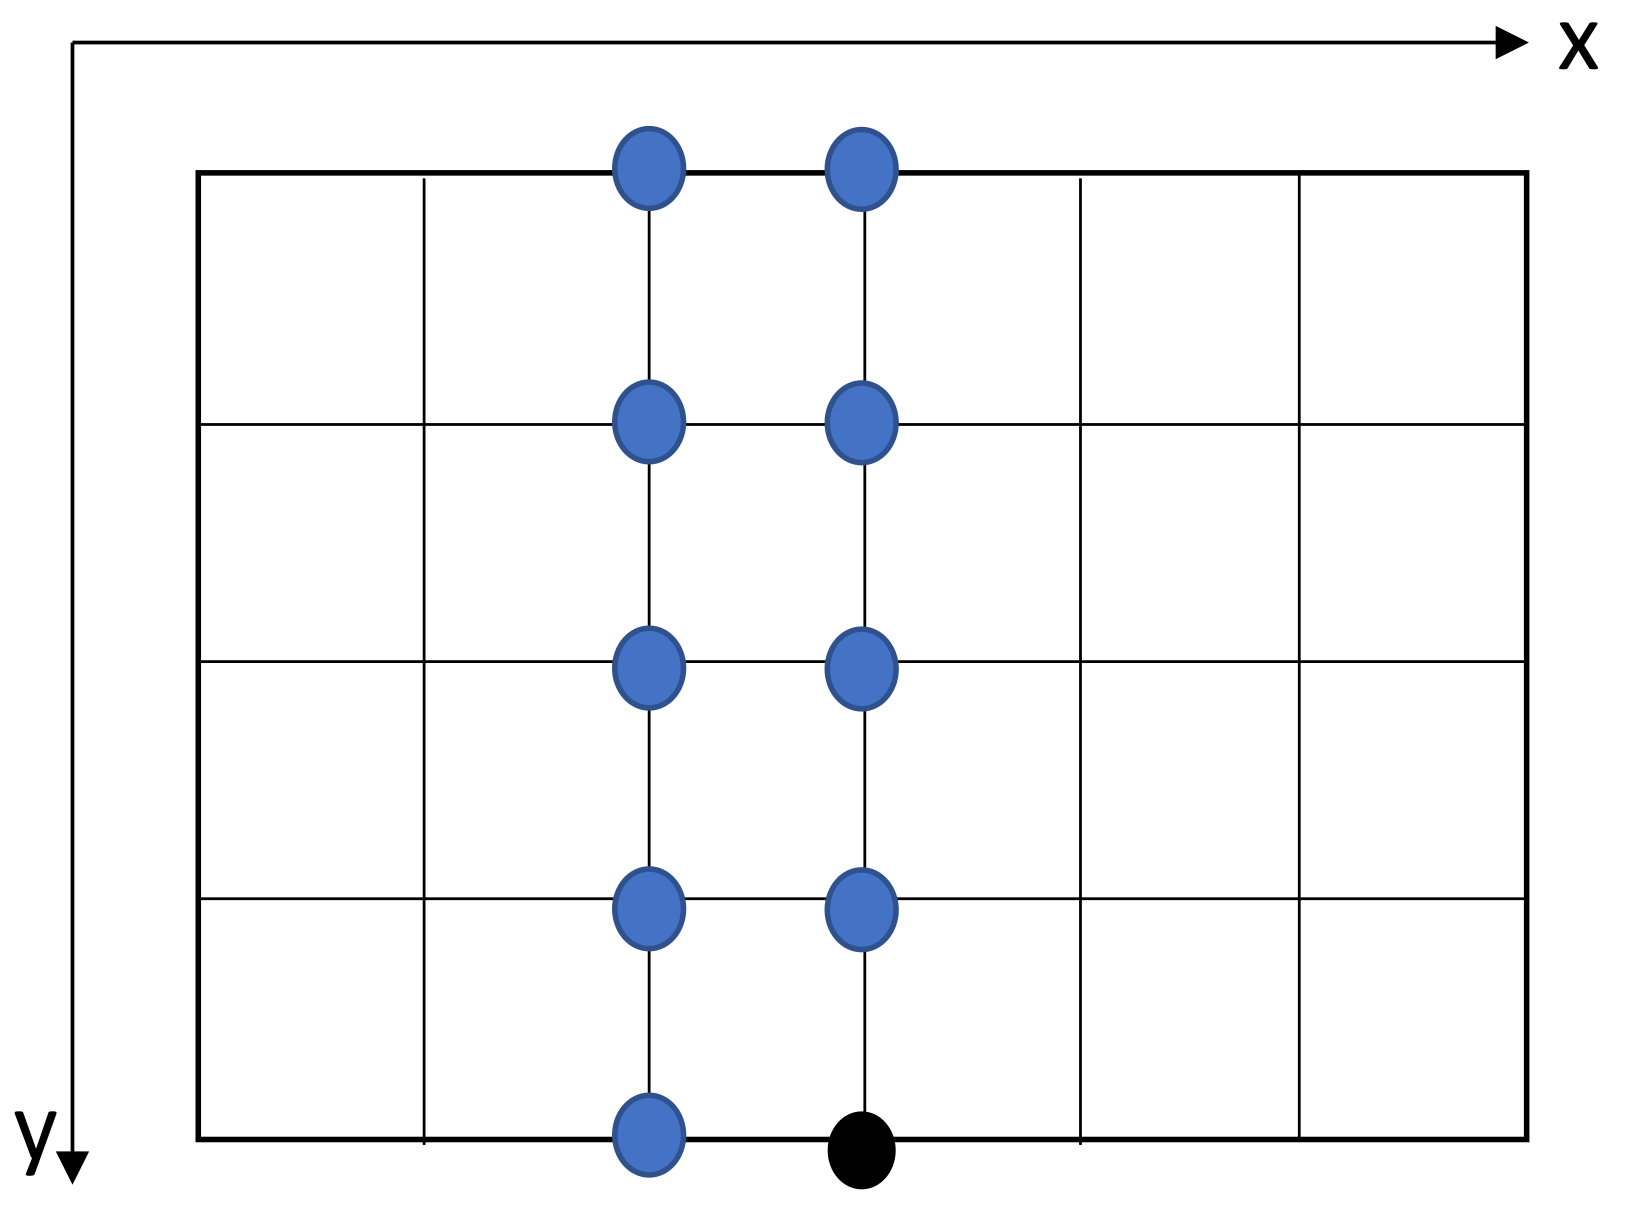
\includegraphics[width=2.5in]{figures/meshbordery2.png}}
    \hspace{1in} 
  \subfigure[$T(2(x_i+2))$]{ 
    \label{fig:subfigmesh3:c} %% label for second subfigure 
    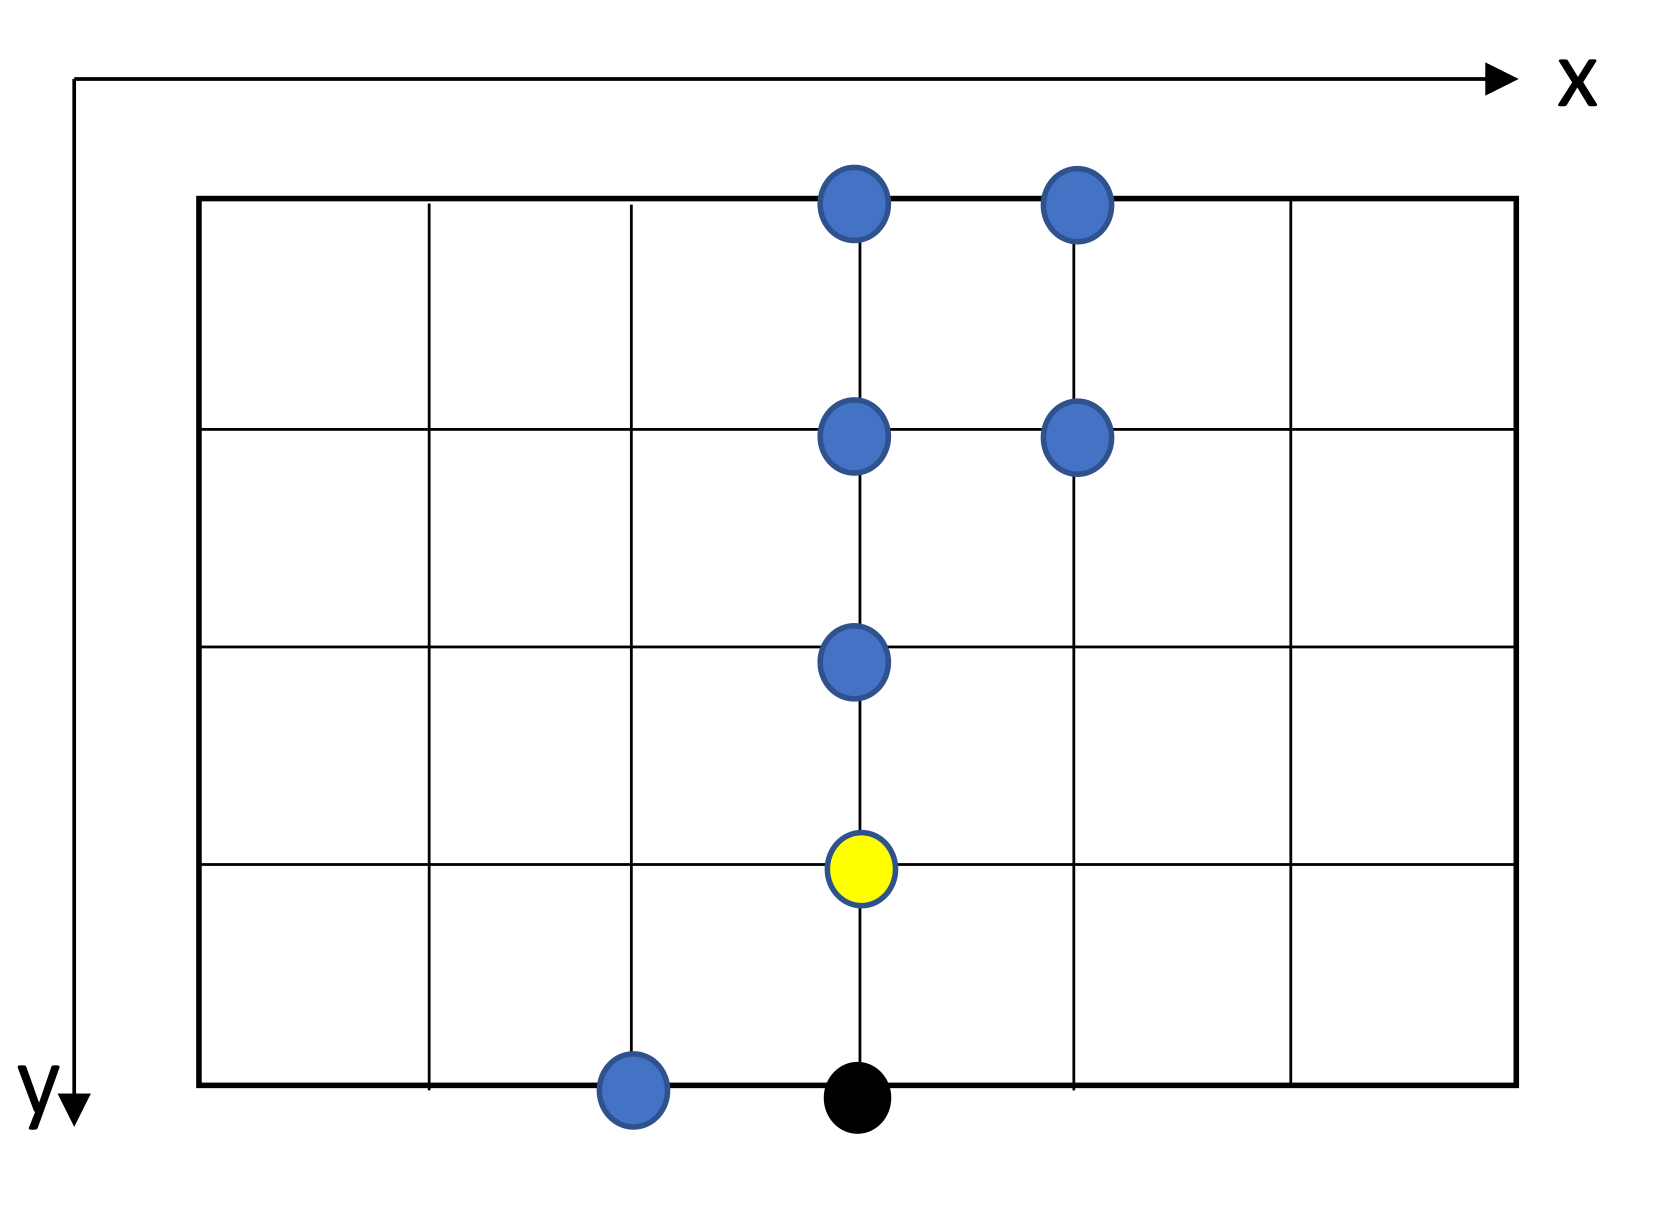
\includegraphics[width=2.5in]{figures/meshbordery3.png}}
%      \hspace{1in} 
  \subfigure[$T(2(x_i+3))$]{ 
    \label{fig:subfigmesh3:d} %% label for second subfigure 
    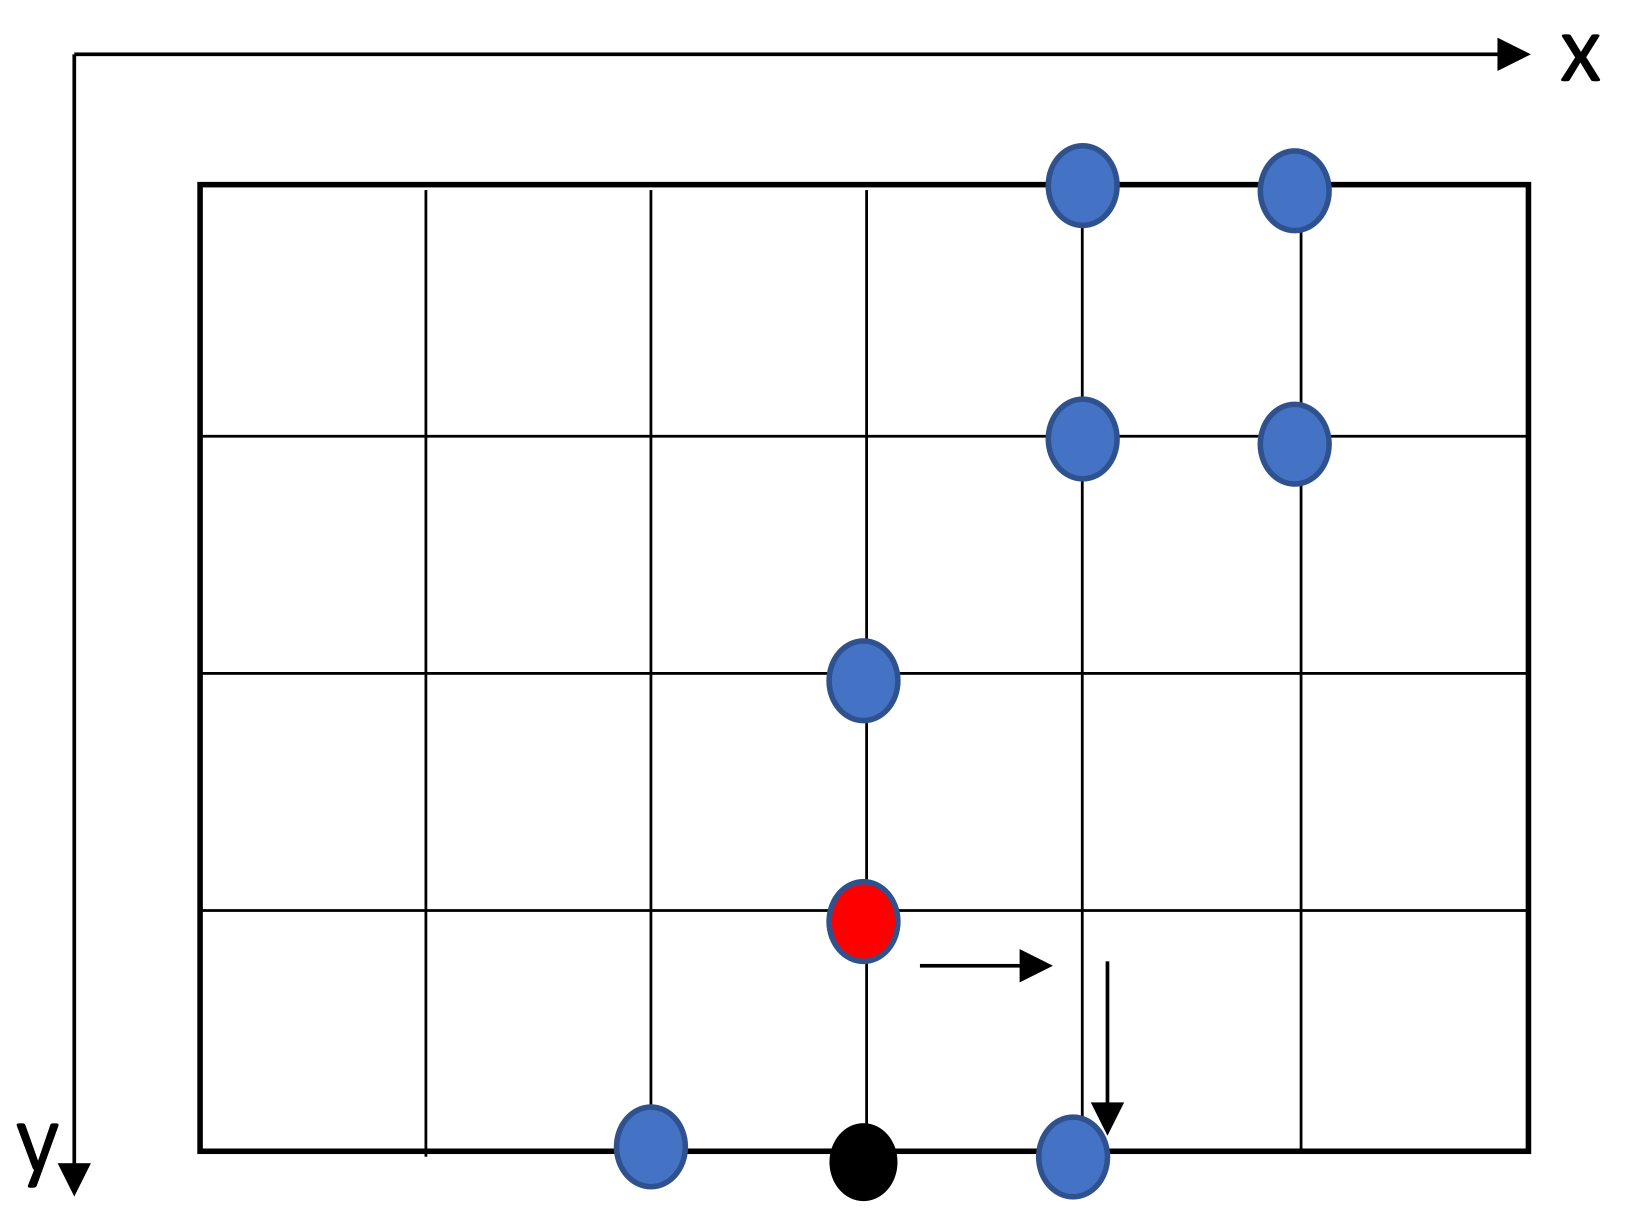
\includegraphics[width=2.5in]{figures/meshbordery4.png}}
      \hspace{1in} 
  \subfigure[$T(2(x_i+3)+1)$]{ 
    \label{fig:subfigmesh3:e} %% label for second subfigure 
    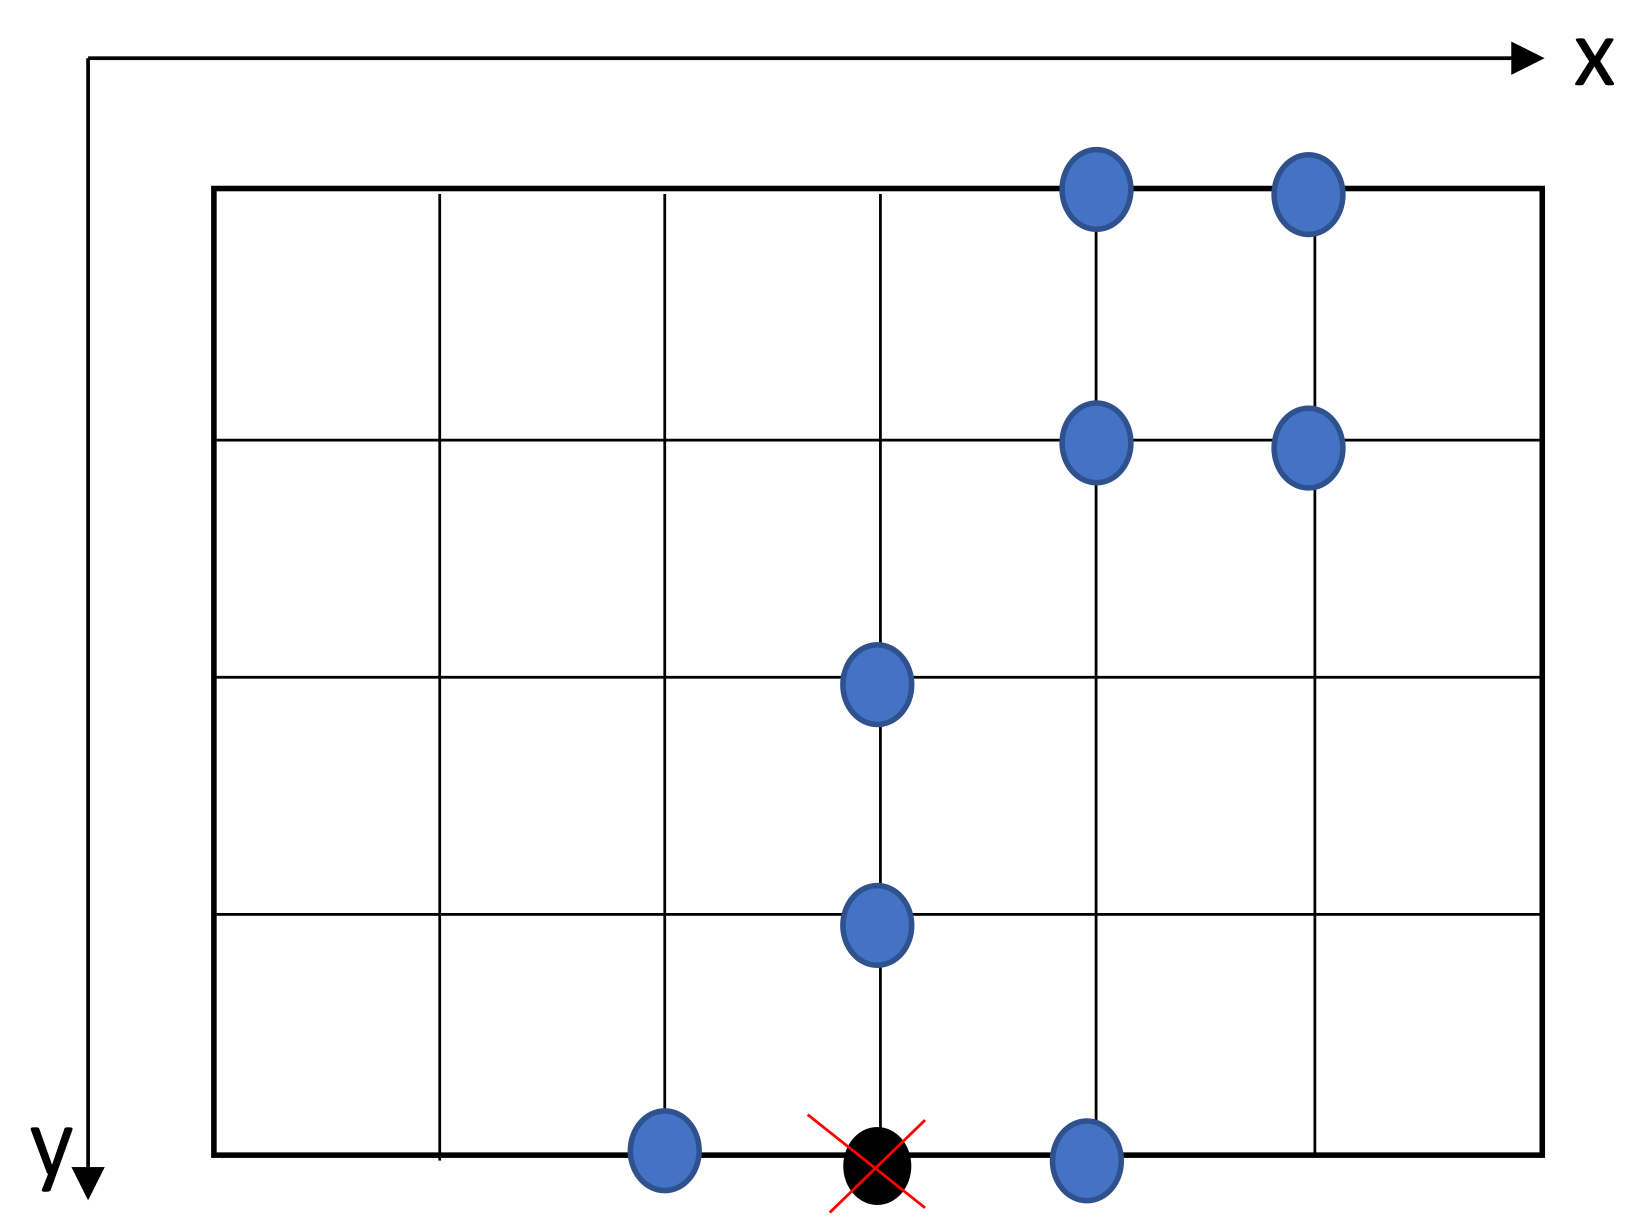
\includegraphics[width=2.5in]{figures/meshbordery5.png}}
  \caption{Arrangement of agents in elimination phase when the new formed BV resides in a border node (when $y=1$ or $y=d_2-1$ ) } 
  \label{fig:subfigmesh3} %% label for entire figure 
\end{figure}

\item Case 4: When $x=d_1$ and $y=1$ or $y=d_2-1$ (a corner node becomes a new formed BV). For convenience, we only discuss the situation when $y=1$. In this case, agents residing in node $(x-1, y+1)$ and $(x-2, y)$ (let's say agents a,b) receive a BV clone at T(2$x_i$+1). Both of them keep moving for one step and arrive at nodes $(x, y+1)$ and $(x-1, y)$ at T$(2(x_i+1))$.
\begin{figure} [H]
  \centering 
  \subfigure[$T(2x_i+1)$]{ 
    \label{fig:subfigmesh4:a} %% label for first subfigure 
    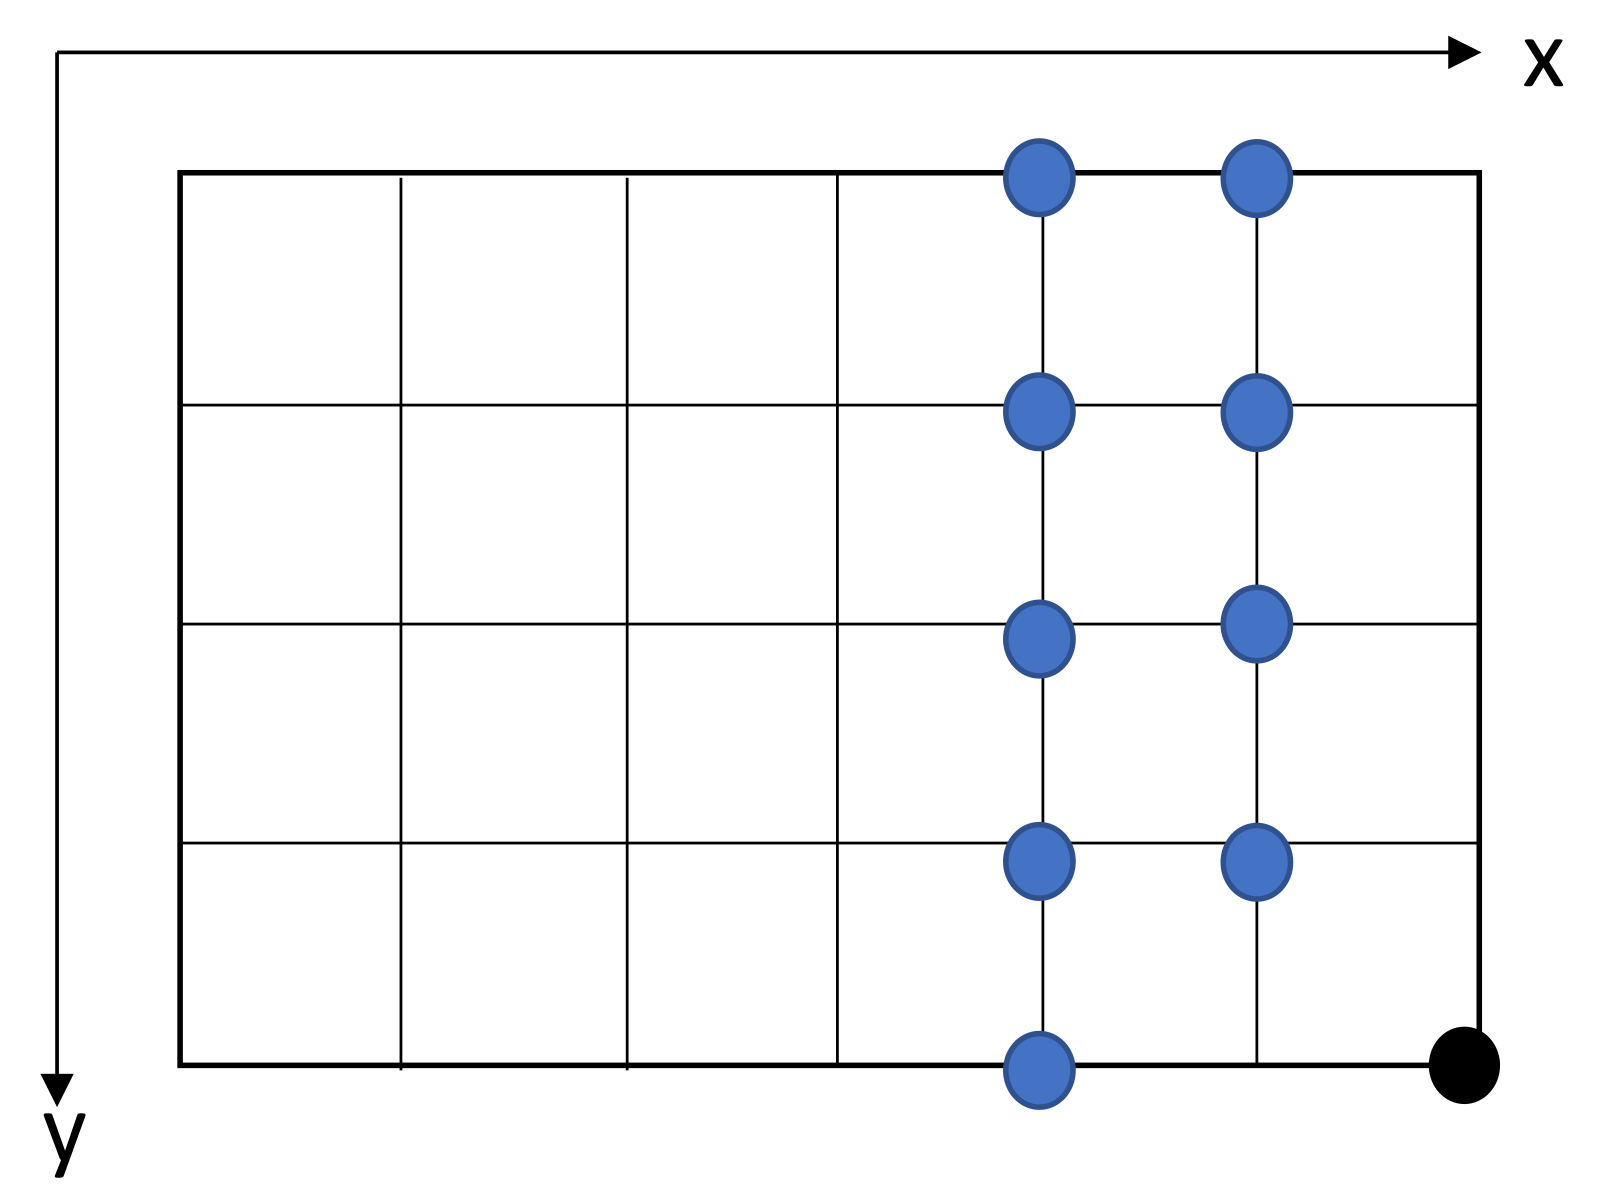
\includegraphics[width=2.5in]{figures/meshcorner1.png}} 
%  \hspace{1in} 
  \subfigure[$T(2(x_i+1))$]{ 
    \label{fig:subfigmesh4:b} %% label for second subfigure 
    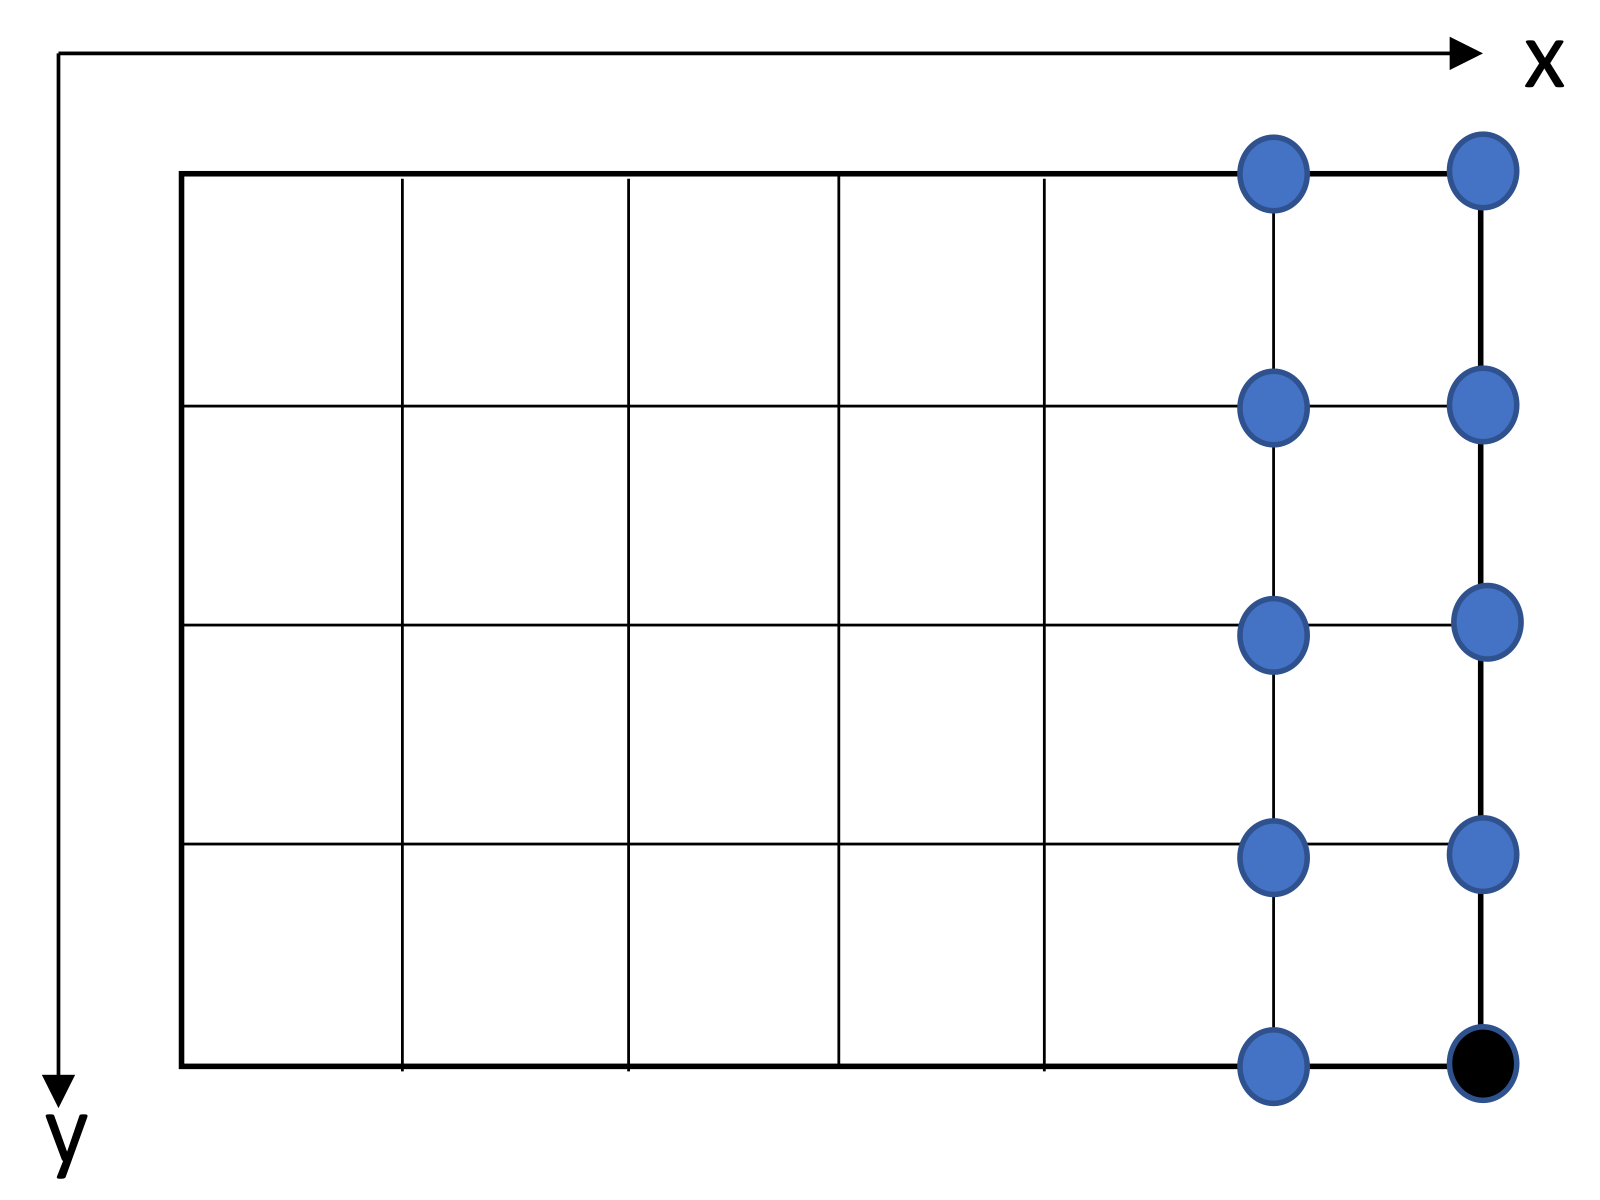
\includegraphics[width=2.5in]{figures/meshcorner2.png}}
    \hspace{1in} 
  \subfigure[$T(2(x_i+2))$]{ 
    \label{fig:subfigmesh4:c} %% label for second subfigure 
    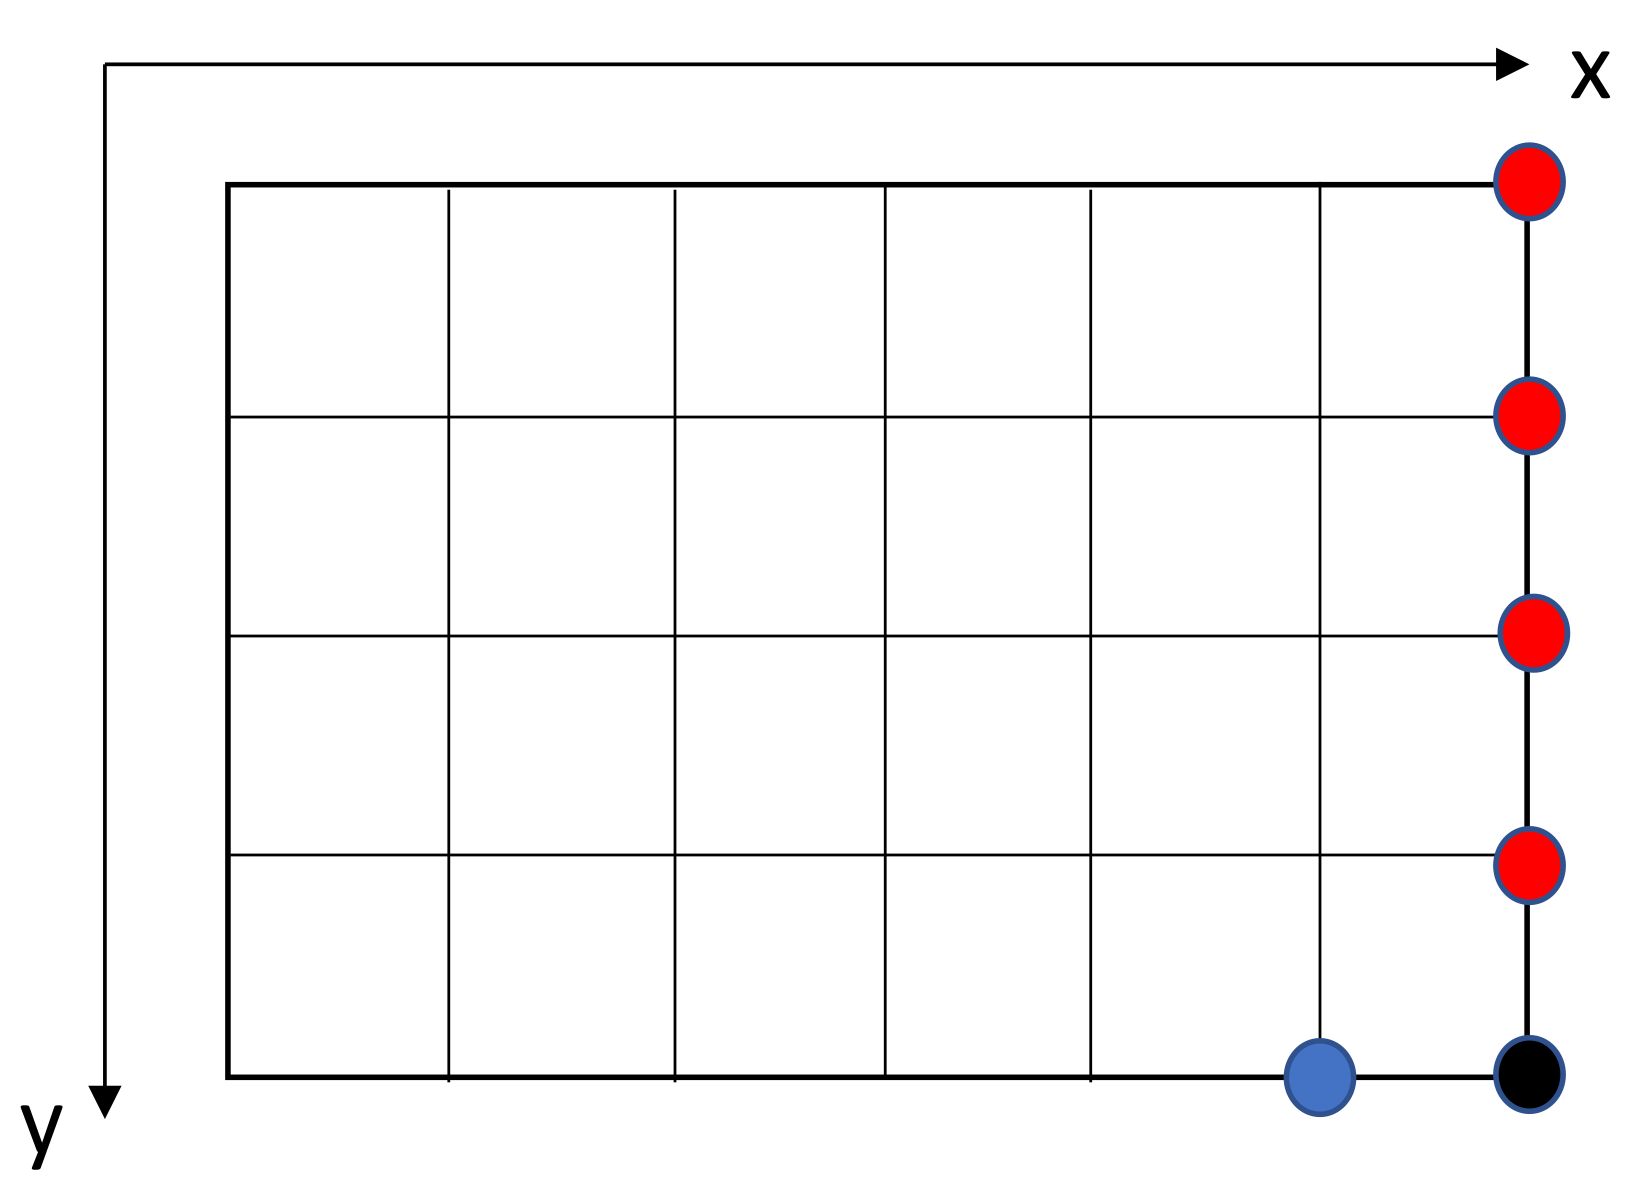
\includegraphics[width=2.5in]{figures/meshcorner3.png}}
%      \hspace{1in} 
\subfigure[$T(2(x_i+2)+1)$]{ 
    \label{fig:subfigmesh4:d} %% label for second subfigure 
    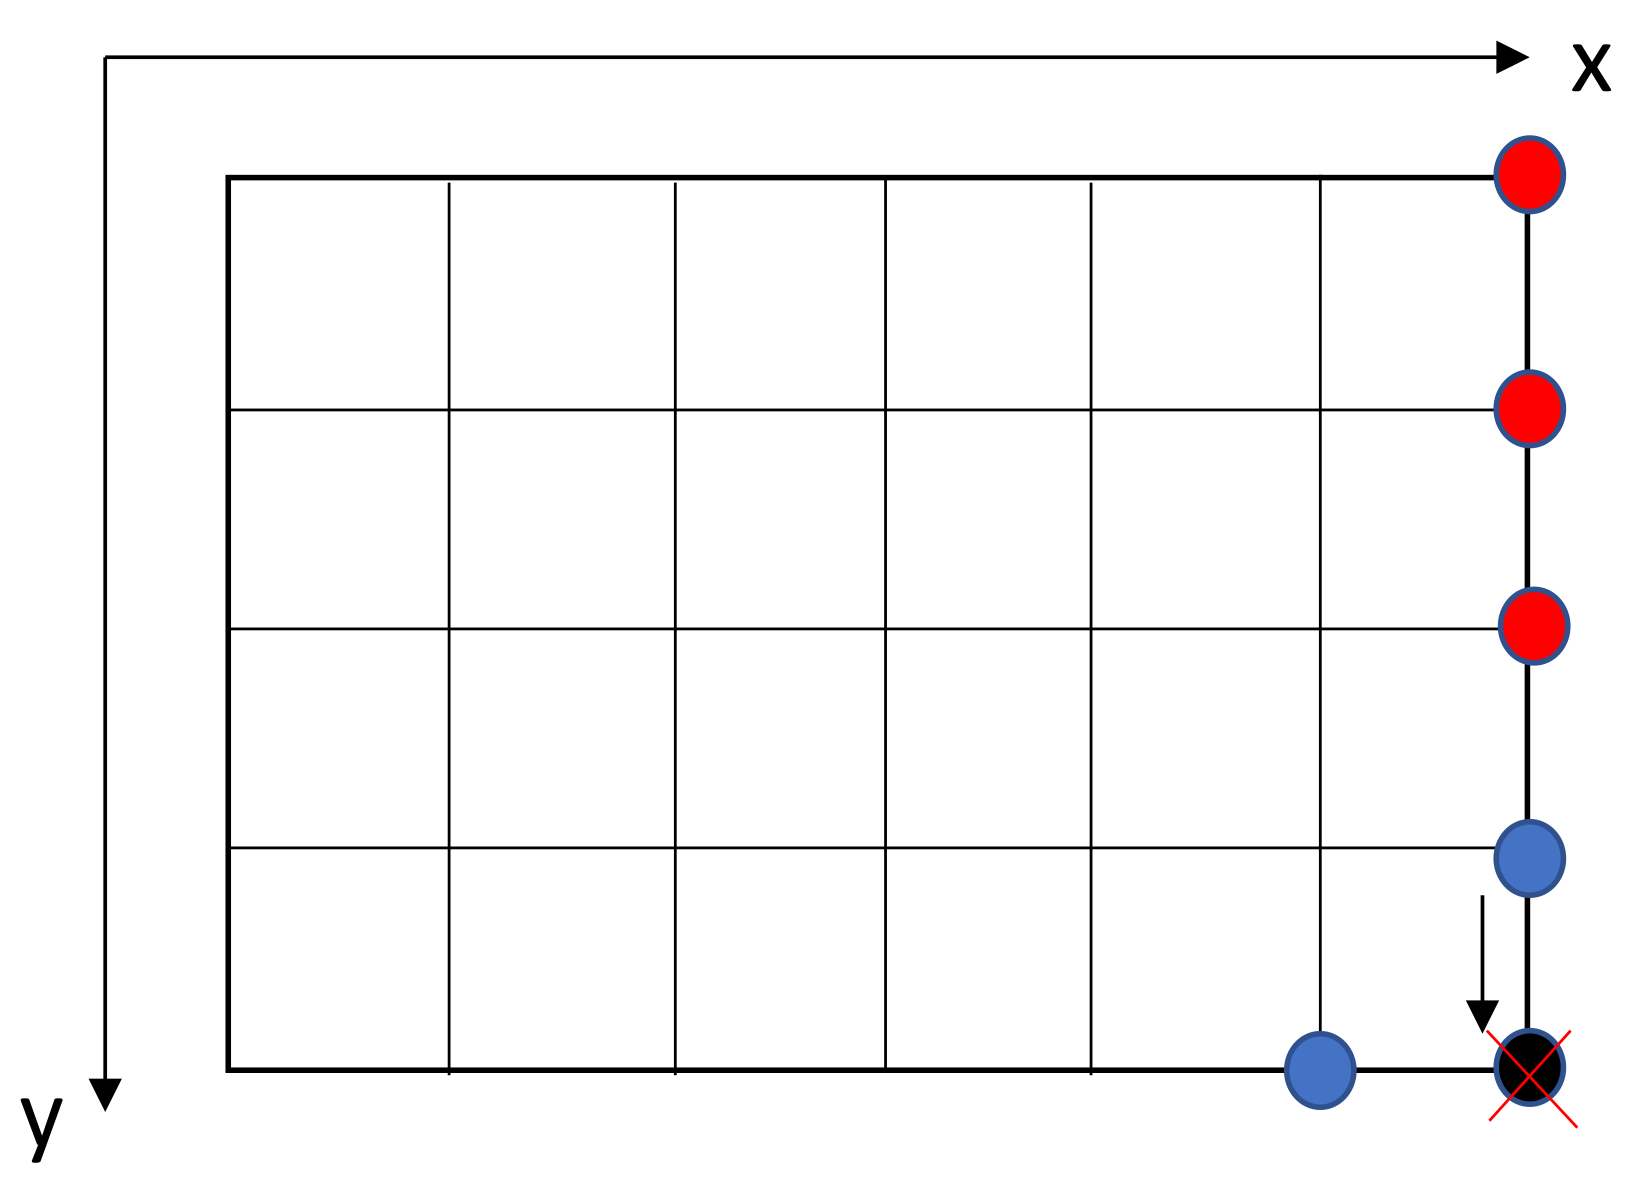
\includegraphics[width=2.5in]{figures/meshcorner4.png}}
    \caption{Arrangement of agents in elimination phase when the new formed BV resides in a corner (when $x=d_1$ and $y=1$ or $y=d_2-1$)} 
  \label{fig:subfigmesh4} %% label for entire figure 
\end{figure}
\end{itemize}

\noindent{\bf Analysis and Comparing}
\begin{theorem}
Mesh contamination algorithm performs a decontamination of a mesh (size of $n=d_1\times d_2(d_1>2,d_2>2)$ using $k=2\sqrt{n}$ agents and at most 1 casualties.
\end{theorem}
\begin{proof}
Let $v=(x, y)$ be the node containing the BV. When one of the agent in the exploring group moves to $v$, it will be destroyed and the BV will move to all neighbours of $v$. If $x=1$, then the neighbours $(x, y+1)$, $(x, y-1)$ and $(x+1, y)$ are protected by agents and neighbour $(x-1, y)$ actually does not exist; if $x>1$, then neighbours $(x, y+1)$, $(x, y-1)$ and $(x-1, y)$ are protected by agents. So when the clones of BV moves to the neighbours of $v$, those contain a agent will not be infected by the BV clone; this means that the BV can safely move only to the unexplored neighbours of $v$, of which are at most one. In other words, after $v$ is explored, at most one BV node are formed. According to our elimination strategy, the new formed BV node can be surrounded and destroyed using at most five agents: one to enter a BV and four to protect the neighbours. Since we have one new formed BV, the number of agents participating in the elimination phase is at most five. In addition to the agent destroyed by the original BV, the number of agent needed to complete the elimination phase is at least six. Since we employ $k=2d_1$ ($d_1\geq 3$) which means at the beginning we have at least six agents, so $2d_1$ agents are enough for the decontamination algorithm.
\end{proof}
Let us now consider the number of movements.
\begin{theorem}
Parallel mesh decontamination algorithm performs a BV decontamination of a mesh of size n with at most $2n-\sqrt{n}+O(1)$ movements in time at most $\sqrt{n}+11$.
\end{theorem}
\begin{proof}
Let $v=(x, y)$ be the BV node, and let the size of the grid be $n=d_1\times d_2$. Let us first consider the number of movements performed during the shadowed exploration. Since all the agents simply move EAST at the beginning of T(2n) ($n=0,1, \dots , d_2-1$), the travelling distance is $x$ for agents in the exploring group ({em EA}) and $x-1$ for agents in the shadowing group({em SA}). We have $d_1$ {\em EAs} and $d_1$ {\em SAs}, then we have an overall cost of at most $d_1\times (2x-1)$ movements for this phase.
Consider now the number of movements performed for Surrounding and Elimination. In this part, we only compute the movements of the agents who participate in the Surrounding and Elimination. More specifically, we simply ignore the movements of the agents who do not know the existence of the BV in the whole process. As we discuss in the Elimination phase, when the new formed BV is located in a interior node, ten movements are needed in this phase; when the new formed BV is located in a border node (let' s say $(a, b)$), then eight movements are needed when $a=d_1, 2< b <d_2-1$ and eleven movements are needed when $2< a <d_1,b=1 or b=d_2-1$; when the new formed BV is located in a corner node, then five movements are needed in this phase. Hence $O(1)$ movements are performed in this phase.
In total we have that the number of movements is at most $d_1 \times(2x-1)+O(1)\leq \sqrt{n}\times(2\sqrt{n}-1)+O(1)$, which is $2n-\sqrt{n}+O(1)$.\\
As for the time complexity. The time required for the exploration phase is equal to the number of movements of EA, which is $d_1$; the time required for the surrounding and elimination phase is at most eleven. So in total the parallel mesh decontamination algorithm terminate in time at most $\sqrt{n}+11$. 
\end{proof}

Now we make some comparison between our strategy and the sequential strategy.

\begin{table} [hbtp]
\caption{Appointment Card}
\label{table:AptCard}
\centering
\tabulinesep=2mm
\begin{tabu} to 140 mm {|X[6,c]|X[4,l]|X[4,l]|X[4,l]|X[4,l]|} \hline 
%\begin{tabular}{|c|l|} \hline 
& The number of agent & The time cost & The number of movement & The casualties \\ \hline
{\em PBVD-2G}   & $2\sqrt{n}$   & $\sqrt{n}+11$ & $2n-\sqrt{n}+O(1)$   & 1        \\ \hline
{\em BVD-2G} & 7    & $3n$          & $9n+O(1)$     & 3              \\ \hline
\end{tabu}
%\end{tabular}
\end{table}

\subsection{Multi-Dimensional Grid}
Let $M$ be a q-dimensional grid of size $d_1\times\ldots\times d_q$ and let each node of $M$ be denoted by its coordinates $(x_1,\ldots,x_q)$, $1\leq x_i\leq d_i$. The algorithm, called {\em PBVD-qG}, follows a general strategy similar to the one described in Section 4.2.1: a safe exploration with shadowing, followed by a surrounding and elimination phase. 













%%%%%%%%%%%%%%%%%%%%%%%%%%%
\chapter {Parallel Black Virus Decontamination in Chordal Ring}
\label{TL}
%%%%%%%%%%%%%%%%%%%%%%%%%%%
 

\section{Introduction}
In this chapter, we discuss parallel strategy on BVD problem in chordal ring. A chordal ring is a circulant graph with $d_1=1$, i.e., it is an augmented ring, and will be denoted by $C_n(1, d_2, ..., d_k)$. More specifically, in chordal ring each node is directly connected to the nodes at distance $d_i$ by additional links called chords. The link connecting two nodes is labeled by the distance that separates these two nodes on the ring. 
For convenience, if we say the agents or the clones move along chord $i$, then they actually move along $d_i$. If we say the agents or the clones move $i$, then they actually move along chord $d_x$ with its length equal to $i$. Let us donated by $d$ the half degree of the chordal ring (for example, for the chordal ring structure $C_n(1,2,4,5)$, $d=4$), by $l$ the length of the longest chord of the chordal ring (for example, for the chordal ring structure $C_n(1,2,4,5)$, $l=5$). In order to simplify the process, we assume that all the nodes in the network are marked with a number: the starting point is marked 0, then the second node is marked 1\ldots.Our goal is to minimize the time to complete the whole decontamination process and at the same time the casualties. In order to do that, we propose a parallel strategy for decontaminating the chordal ring. Agents are not allowed to communicate with each other unless they are in the same node so the protocol should enable agents in different nodes to move properly. That is, the route of every agent is different but they are served to explore the network; when a BV is triggered, other agents should bypass the new-formed BVs. We give simple but efficient solution to deal with the problem with acceptable cost. 
In the elimination phase, we are interested in executing it also parallelly. But in this case, an tricky situation might happen: supposing that the sites of the two clones are connected, in this case, after these two clones are triggered, one of their clones spread to another sites and since the agents sent to destroy them die, these two sites are empty when the second round clones arrive, which make our decontamination invalid. In order to solve this problem, we make an assumption when we talk about the parallel strategy in elimination phase in chordal rings: when a BV is triggered at $T_i$, it takes negligible time for its clones to reach all its neighbours, for example, at $T_i$.  Since time cost in the elimination phase is negligible comparing to the exploring phase if n is large enough, it would be much simple to execute the elimination sequentially. That is, instead of destroy all the clones at the same time, we decontaminate them on by one. Also, in the elimination phase, in order to save the number of agents, we chase all the $Keep\,Moving$ agents (explained in section Surrounding and Elimination) back. It is obvious that we may cost some time here, if the execution time is of great important to us and we care less the number of agents we employ, then we may carry enough agent at the beginning and start the elimination phase right after the exploring phase. In conclusion, In the exploring phase, we have one strategy, but in the elimination phase, we provide several strategies: 1) chasing back the $Keep\,Moving$ agents and decontaminating the BVs sequentially 2) chasing back the $Keep\,Moving$ agents and decontaminating the BVs parallelly 3) start to decontaminating the BVs right after the exploring phase and do it parallelly 4) start to decontaminating the BVs right after the exploring phase and do it sequentially. The cost of each strategy including time, number of agents, casualties would be analyzed in the section Analysis and Comparing.

\section{Shadowed Exploration}
\noindent{\bf Initialization }\\
The chordal ring is a complete symmetrical structure, so we can randomly choose a node $x_0$ as the start node. Initially, we place $2d$ agents at node 0, 1, \ldots , $2d-1$ (first round). Agents residing in nodes from $0$ to $d-1$ are in shadowing group, while from $d$ to $2d-1$ are in exploring group. If none of the agent is destroyed, we then place $d$ agents at nodes 0,1, \ldots, $d-1$ (second round). If not, we can easily know the location of the BV and employ agents to surround the new formed BVs, then destroy them permanently. Only the agents employed in the first round move in the exploring phase. The agents employed in the second round remain dormant, guarding the nodes to guarantee the monotone. 

\noindent{\bf Route of the agent in exploring phase}\\
We separate the time of exploring phase into two part: moving time and notice time. In the whole phase of exploring phase, they are arranged as below: $T_{move\_1}$, $T_{notice\_1}$, $T_{notice\_1'}$, $T_{notice\_1''}$, $T_{move\_2}$, $T_{notice\_2}$, $T_{notice\_2'}$, $T_{notice\_2''}$ ...More specifically, every cycle contains one unit of time for moving and three units of time for notice. We discuss why we arrange the time as above and what exactly the agents do in the notice time later. 

In chord ring $C_n(1, d_2, \ldots, d_k)$, all the agents in the array move along their longest chord $d_k$ in $T_{move\_i}$. That is, agents move along $d_k$ in $T=1+4t$ $(t\in \mathbb{N})$.  An example of how agents move in chordal ring $C_n(1, 2 , 4, 5)$ at $T_{move\_i}$ in exploring phase is shown in Fig.\ref{fig:subfig1}. \\

\begin{figure} [H]
  \centering 
  \subfigure[Arrangement of agents at $T_{move\_i}$]{ 
    \label{fig:subfig1:a} %% label for first subfigure 
    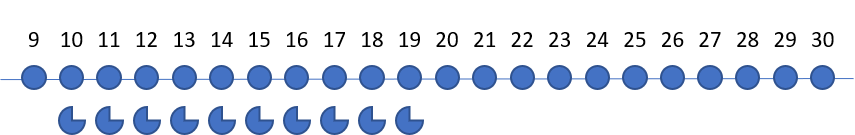
\includegraphics[width=3.0in]{figures/chordal_a_l.png}} 
  \hspace{1in} 
  \subfigure[Arrangement of agents at $T_{move\_{i+1}}$]{ 
    \label{fig:subfig1:b} %% label for second subfigure 
    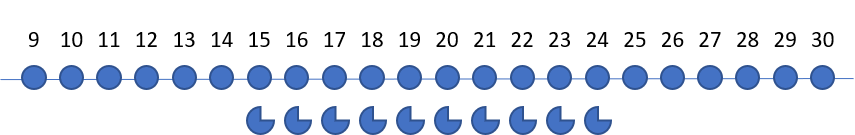
\includegraphics[width=3.0in]{figures/chordal_a1_l.png}}
  \caption{Arrangement of agents when moving} 
  \label{fig:subfig1} %% label for entire figure 
\end{figure}

\noindent{\bf Three\,Jump\,Notifying\,Technique}
In the strategy of BV decontamination exploring the network sequentially, two agents explore the graph (exploring agent and leader agent) and they follow the casual walk. That is, exploring agent moves to the next node in its route, and if the node is safe, it moves back to the leader agent, and then move forward to that safe node together. In this case, if the leader agent does not meet the exploring agent in next $T$ after the exploring agent moves forward, the leader agent learns that the original BV resides in the next node so it stop moving. \\

But in our model, we employ $2d$ agents in the exploring phase, if they are not properly informed when one agent is destroyed by BV, in their next step of moving, some of them may be destroyed by the new formed BVs. In order to avoid the casualties, we propose $Three\,Jump\,Notifying\,Technique$ to properly notify the agents who will move to the new formed BVs.\\

To explain it more clearly, let us take the node where the original BV resides as the original of the one-dimensional coordinate system. In a chordal ring $C_n(1, d_2, \ldots,  d_k)$, if the original BV is triggered, the clones of it spread to nodes whose coordinates are $-d_k$, $-d_{k-1}$, \ldots, $-d_2$, $-1$, $1$, $d_2$, \ldots, $d_{k-1}$, $d_k$. Obviously the nodes whose coordinates are $1$, $d_2$, \dots, $d_{k-1}$, $d_k$ may become the BV (Possible BV Nodes) now, our goal is to notify the agents which will move to these nodes ($Risky\,Agent$) to stop. The coordinates of $Risky\,Agent$ ($RA$s) are $1- d_k$, $d_2-d_k$, \ldots, $d_{k-1}-d_k$, $d_k-d_k$ (which is exactly the coordinate of the original BV) respectively. It is obvious that not all of the nodes from $1$ to $d_k$ become BV nodes after the triggering because there might be some agents already there, but since notifying all the $Risky\,Agents$ does not add more cost comparing to notifying some of them, in our strategy, we notify all of the $RA$s. Let us donate one of the possible BV nodes by $d_i$, and in our $Three\,Jump\,Notifying\,Technique$, agent residing in node $-d_i$ ($Notification\,Agent$) is employed to notify the agent residing in node $-d_k+\left |d_i\right |$ (RA) who will move to the BV node. \\
We show that $Notification\,Agent$ (NA) are able to meet $RA$ in three steps: $-d_i\xrightarrow[]{move\left | d_i \right |}0\xrightarrow[]{move\,along\,chord\,k}-d_k\xrightarrow[]{move\,\left | d_i \right |}-d_k+\left|d_i\right|$. In this case, the notifying route of the $NA$ whose coordinate is $-d_k$ is $-d_k{\rightarrow}0{\rightarrow}-d_k{\rightarrow}0$ . We would make some modification of this agents route in the $Surrounding\,and\,Elimination$, but now let us assume it still follow the route above. The whole process of $Three\,Jump\,Notifying\,Technique$ in chordal ring $C_n(1, 2, 4, 5)$ is shown in Fig.\ref{fig:subfig}. \\

\begin{figure} [H]
  \centering 
  \subfigure[Arrangement of agents at $T_{move_i}$]{ 
    \label{fig:subfig:a} %% label for first subfigure 
    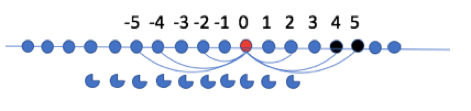
\includegraphics[width=2.5in]{figures/tjt1.png}} 
  \hspace{1in} 
  \subfigure[Arrangement of agents at $T_{notify_i}$]{ 
    \label{fig:subfig:b} %% label for second subfigure 
    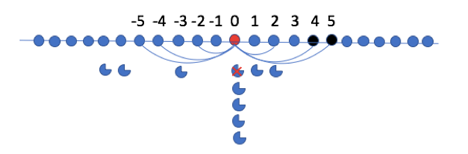
\includegraphics[width=2.5in]{figures/tjt2.png}} \
  \hspace{1in} 
  \subfigure[Arrangement of agents at $T_{notify_i'}$]{ 
    \label{fig:subfig:c} %% label for second subfigure 
    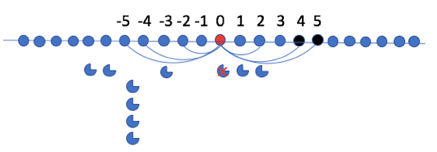
\includegraphics[width=2.5in]{figures/tjt3.png}} 
  \hspace{1in} 
  \subfigure[Arrangement of agents at $T_{notify_i''}$]{ 
    \label{fig:subfig:d} %% label for second subfigure 
    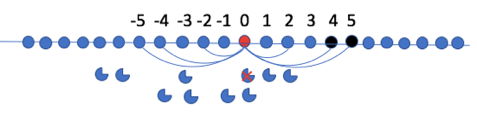
\includegraphics[width=2.5in]{figures/tjt4.png}} 
  \caption{The whole process of the $Three\,Jump\,Notifying\,Technique$ in chordal ring $C_n(1, 2, 4, 5)$} 
  \label{fig:subfig} %% label for entire figure 
\end{figure}


If the original BV residing in the red node, then once an agent moves to it, the agent and the BV are destroyed but the clones of the BV spread to all its neighbours. According to our technique, nodes whose coordinates are $1$, $2$, $4$, $5$ become $Possible\,BV\,Nodes$; agents residing in nodes $-4$, $-3$, $-1$, $0$ are the $RA$s; agents residing in nodes $-5$, $-4$, $-2$, $-1$ are the $NA$s. The routes for agents residing in nodes $-5$, $-4$, $-2$, $-1$ are $-5{\rightarrow}0{\rightarrow}-5{\rightarrow}0$; $-4{\rightarrow}0{\rightarrow}-5{\rightarrow}-1$; $-2{\rightarrow}0{\rightarrow}-5{\rightarrow}-3$; $-1{\rightarrow}0{\rightarrow}-5{\rightarrow}-4$ respectively.\\

\noindent{\bf Safe Exploring with Three\,Jump\,Notifying\,Technique}

After the initialization, agents employed in the first round move as the route we introduced in ``Route of the agent in exploring phase''. When one of the agents is destroyed at $T_{move_i}$, then $Three\,Jump\,Notifying\,Technique$ begins. In ``Route of the agent in exploring phase'', we say that in the exploring phase every cycle contains one unit of time for moving and three units of time for notifying. Actually, the three units of time for notifying are reserved for $Three\,Jump\,Notifying\,Technique$, even though it only executes when one of the agents is destroyed. In another word, before encountering a BV, all the agents just stay where they are in the notifying time.
After executing the $Three\,Jump\,Notifying\,Technique$, the $NA$ moves back to where they are before the notification. For example, in the example in $Three\,Jump\,Notifying\,Technique$, $NA$ residing in node $-1$ moves back to node $-4$ following the reverse route in the notifying phase which is $-1{\rightarrow}-5{\rightarrow}0{\rightarrow}-4$. 

\section{Surrounding and Elimination}
It is obvious that not all the agents are informed to stop so we call the agents continuing to move the $KeepMoving$ agents. In this section, we introduce the process of eliminating the BVs after the original BV is triggered. For the purpose of saving the number of agents, we prefer to chase the $Keep\,Moving$ agents, but it is not necessary to complete the process especially when you care most the execution time, you can carry enough number of agents so you can proceed the $Surrounding\,and\,Elimination$ immediately. The number of agents that should be carried in order to successfully proceed the $Surrounding\,and\,Elimination$ is discussed later in section Analysis and Comparing. Now we introduce how to chase the $KeepMoving$ agents.

\subsection{Notifying Moving Agents}

\noindent{\bf Overview of the Notifying Moving Agents}

When the $Shadowed\,Exploring$ ends, it is possible that some of the agents in the array are not informed and do not realize the existence of the BV, so they keep moving following the routes in $Shadowed\,Exploring$  phase but it is obvious that they would not encounter any BV. In order to reduce waste, we employ the agent who receives the clone from chord $d_k$ ($Coordinate\,Agent$) to notify the other $Keep\,Moving$ agents to move back to their position when the BV is triggered. Now we introduce how we choose the $Coordinate\,Agent$($CA$)and how the $CA$ notifies the other agents.\\

\noindent{\bf The Process of the Notifying Phase of the Coordination Agent}

We can see that the relative position of agents does not change when they keep moving along the longest chord. For example, agents residing in nodes 1, 5, 10 (noted as $A1$, $A5$, $A10$) move along the longest chord and then $A5$ moves forward for one step. The relative position of them would be exactly the same as the situation where all of them remain dormant except $A5$ moves forward for one step. Now we discuss how the $CA$ notify all the $Keep\,Moving$ agents assuming they are dormant and then make some modification to fit the scenario where the $CA$ notifies the $Keep\,Moving$ agents. The problem we need to solve is that given a range within which the agents are in and a $CA$ located in this range, let the $CA$ to notify all the agents in this range. In a chord ring $C_n(1, d_2, \ldots, d_k)$, the $CA$ sets a $Notification\,Window$ using the modular arithmetic. Let us assume the number of the node where the $CA$ resides in is $x$, the number of the nodes where should be marked the $Beginning\,Flag$ and the $End\,Flag$ are $y$ and $z$. 

The relations between $x$, $y$, $z$ should be as follow: 

\begin{itemize}
\item $y$ is the biggest number which satisfies that it is smaller than or equal to $x$ and that $y$ mod $d_k$ =$0$; 
\item $z$ is the smallest number which satisfies that it is bigger than $x$ and that $z$ mod $d_k$ = $d_{k-1}$.
\end{itemize} 


When the agent is chosen to be the $CA$, it computes its $Notification\,Window$. When we mention marking a flag, it does not mean that the agent has to move to the node to do that but only needs to remember the positions of the two flags in its memory. Also, after the position of the $Notification\,Window$ is set, it remains stable. More specifically, when the $CA$ moves, he does not set another $Notification\,Window$ using its new position. The $CA$ moves step by step to every possible position and notifies the agents to go back if there is one until it realizes that it just passes the $End\,Flag$. After that, he moves along the longest chord anticlockwise to the node marked a $Beginning\,Flag$ and continues moving again step by step to notify agents until it arrives its relative departing node. For example, if the $CA$ starts to notify other from node $x$, then its relative departing node is $x'=x+t\times{d_k}$ ($t\in \mathbb{N}$).

We make some modifications to let the solution fit the real scenario where the agents move along the longest chord: 
\begin{itemize}
\item The Beginning Flag and the End Flag move along the longest chord also to keep the relative position the same. 
\item  When one agent $A1$ moves to a node where there is an agent $A2$ knowing the position of the original BV, $A1$ would be informed and directly moves along the longest chord to its own position. 
\item  Let us assume that the time when the original BV is triggered is $T_{move\_i}$ ($T_{trigger}$), then the $CA$ should remember the $T_{trigger}$ and informs the agents he encounters of it. The agent $A1$ who encounters the $CA$ should remember the time when they encounter ($T_{notify\_now}$) and stop moving until next $T_{move}$ when it will meet another agent $A2$. Then $A1$ moves along $d_k$ anticlockwise for $T_{move\_now}-T_{trigger}$ times while $A2$ moves for $T_{move\_now}-T_{trigger}+1$ times. 
\item When arriving its relative departing position at $T_{move\_a}$, the $CA$ knows that it has finished the task and moves along $d_k$ for $T_{move\_a}- T_{trigger}+1$ times to its position when the original BV is triggered.
\item Let us assume that the time when the BV is triggered is $T_{move\_i}$, the $CA$ starts to move step by step to notify other agents after $T_{move\_{i+2}}$, because we want to ensure the security of the $CA$. If it starts to notify other agents at $T_{move\_{i+1}}$, it might encounter a BV. Also, it should be ensured that the $Keep\,Moving$ agents in the exploring group are in the $Notification\,Window$ of the $CA$, or the $CA$ would never encounter them. We would talk about how to ensure this in next section.
\end{itemize} 

\noindent{\bf Election of the Coordination Agent}

We choose the agent who receives a BV clone from its chord $d_k$ to be the $CA$, which means when an agent receives a BV clone from its longest chord, then it realizes that it is chosen as the $CA$. We know that, the notifying phase starts from $T_{move\_{i+2}}$ assuming the time when the BV is triggered is $T_{move\_i}$, which means the notifying phase begins only after all the $Keep\,Moving$ agents move twice. At $T_{move\_{i+2}}$, all the $Keep\,Moving$ agents are in a $Notification\,Window$ from nodes $d_k\times(move\_{i}+1)\,to\,d_k\times(move\_{i}+1) + d_{k}-1$, and let us donate it by $Initial\,Notification\,Window$. The $CA$ would directly move to any node in $Initial\,Notification\,Window$. Now we propose three kinds of routes for the $CA$ to move to his destination:

The coordinates of the positions where the clones spread are: $x-d_k$ (which is the coordinate of the $CA$), $x-d_{k-1}$, $x-d_{k-2}$, \ldots, $x-1$, $x+1$, $x+d_2$, \ldots, $x+d_{k-1}$, $x+d_{k}$ supposing the coordinate of the original BV is $x$ and we are in a chordal ring $C_n(1, d_2,\ldots, d_k)$.
 Now we describe three scenarios:
\begin{itemize}
\item Scenario 1: The last agent of the $Exploring\,Group$ is destroyed by the BV and the positions of the clones satisfy: $x-d_{k-1}+d_{k}=x+1$, $x-d_{k-2}+d_{k}=x+d_2$, \ldots, $x-1+d_{k}=x+d_{k-1}$. 
\item Scenario 2: The last agent of the $Exploring\,Group$ is destroyed by the BV and the at least one pair of the positions of the clones does not satisfy: $x-d_{k-1}+d_{k}=x+1$, $x-d_{k-2}+d_{k}=x+d_2$, \ldots, $x-1+d_{k}=x+d_{k-1}$. 
\item Scenario 3: One of the agents in the $Exploring\,Group$ except the last agent is destroyed by the BV.
\end{itemize}

In scenario 1, the $CA$ needs to move for 5 steps to reach its destination while in the other two scenarios, it only needs to move for 4 steps to arrive the destination. Now we propose the route for each scenario.
\begin{itemize}
\item For $CA$ in scenario 1: Let us donate by $y$ the coordinate of the node in the $Notification\,Window$ set by the original BV which does not receive any clone and his left neighbour receives a clone (the coordinate of it is $y-1$). The $CA$ first moves to the original BV, then to node $y-1$, finally to $y$. After that it only need to move along the chord $d_k$ for twice to reach its destination.
\item For $CA$ in scenario 2: There is at least one pair of the positions of the clones does not satisfy the equations so there should be one node (assuming its coordinate is $z$) who receives a clone from the original BV but node $z+d_k$ is empty. The route now for the $CA$ is first move to the BV, then to node $z$, and then moves along the chord $d_k$ for twice to reach its destination.
\item For $CA$ in scenario 3: The $CA$ here simply need to move for one step to its right neighbour and move along the chord $d_k$ for three times to reach its destination.
\end{itemize}

In any case, the $CA$ can reach its destination within 6 unit of time which is required for the $Keep\,Moving$ agents to move to the $Initial\,Notification\,Window$, so the $CA$ start to chase the $Keep\,Moving$ agents as we introduce from $T_{notify\_{i+2}}$. 

An example of how the agents and the $CA$ move in chordal ring $C_n(1, 2, 7, 11)$is shown in \ref{fig:T29}. For our convenience, in some case, we consider the chordal ring as arranged in rows of $d_k$ where the last node of a row is connected to the first node of the following row and the last node is connected to the first. Depending on the size of the chordal, the last row could be incomplete. So in this matrix, moving down a column corresponding to using the longest chord $d_k$. In the matrix, we also mark the number of nodes.

\begin{figure}[H]
  \centering  
  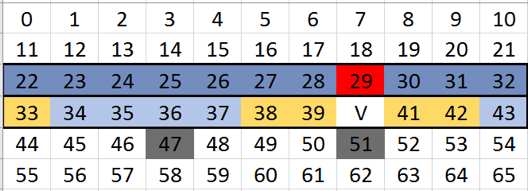
\includegraphics[width=0.6\textwidth]{figures/T29.png}
  \caption{Arrangement of agent at $T_{move\_2}$ when the BV is triggered}\label{fig:T29}
\end{figure}

Yellow nodes are connected to the original BV but guarded by agents while the grey nodes are the new formed BVs. The node marked $V$ is the original BV but now is clean. Agent residing in node 29 receives clone from chord $d_k$ so it knows it is the $CA$ During the notifying time, agents residing in nodes 33, 38, 39 notify agents residing in nodes 36, 31, 30 respectively following the $Three\,Jump\,Notifying\,Technique$ while the $CA$ moves to 28, 39, 50 and finally 61 following the route in scenario 3.

\begin{figure}[H]
  \centering  
  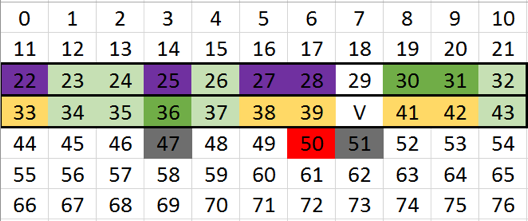
\includegraphics[width=0.6\textwidth]{figures/T50.png}
  \caption{Agents roles after $Three\,Jump\,Notifying\,Technique$ and choosing $CA$. (for convenience, we donate the $CA$ by a red spot, more specifically, node 50 is where $CA$ resides)}\label{fig:T50}
\end{figure}

Agents in purple nodes would be notified at $T_{move\_3}$ and move back. Agents in light green nodes are the $Keep\,Moving$ agents while agent in dark green nodes are informed to stop in $Three\,Jump\,Notifying\,Technique$. In the meantime, the $CA$ moves to node 28, 39, 50, and finally 61. It is obvious that the $CA$ can reach its destination before $T_{move_4}$, so it waits until $T_{notify_4}$ to start its notifying phase. 

\begin{figure}[H]
  \centering  
  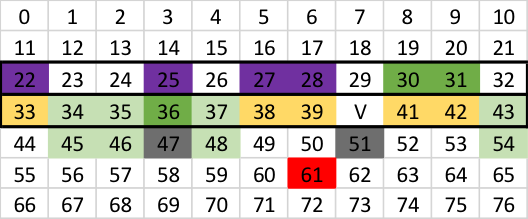
\includegraphics[width=0.6\textwidth]{figures/T611.png}
  \caption{Arrangement of agent at $T_{move\_3}$. The $CA$ has arrived its destination)}\label{fig:T611}
\end{figure}

\begin{figure}[H]
  \centering  
  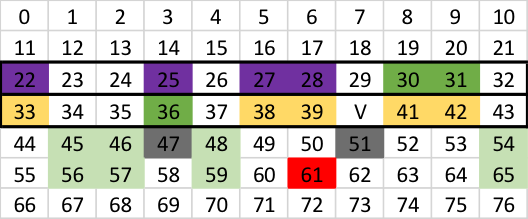
\includegraphics[width=0.6\textwidth]{figures/T612.png}
  \caption{Arrangement of agents at $T_{move_4}$. The $CA$ starts its notice phase}\label{fig:T612}
\end{figure}
In notifying phase, $CA$ starts to notify other $Keep\,Moving$ agents. First, it computes the $Notification\,Window$ which is from node 55 to node 65. Note that the $Notification\,Window$ would move along chord $d_k$ at every $T_{move}$. It moves to node 62 at $T_{notify\_4}$, node 63 at $T_{notify\_4'}$, node 64 at $T_{notify\_4''}$ and to node 75 at $T_{move\_5}$.

\begin{figure}[H]
  \centering  
  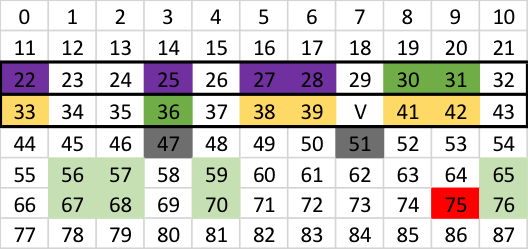
\includegraphics[width=0.6\textwidth]{figures/T75.png}
  \caption{Arrangement of agents at $T_{move_5}$. }\label{fig:T75}
\end{figure}
Again, in the notifying phase, $CA$ moves to node 76 at $T_{notify\_5}$. We can see that it encounters agent residing in node 76, so $CA$ informed it the $T_{trigger}$ which is $T_{move\_2}$. Agent residing in node 76 should remember $T_{notify\_now}$ which is $T_{notify\_5}$ and wait until next $T_{move}$ to inform agent ($Following\,Agent$) who resides in node 65 now but would move to node 76 next $T_{move}$. After encountering its $Following\,Agent$, it informs it to move back along chord $d_k$ for $T_{move\_now}-T_{trigger} +1$ times which is $T_{move\_5}- T_{move\_2}+1$ times while itself moves for $T_{move\_5}$- $T_{move\_2}$ times. 
At $T_{T_{notify\_5'}}$ when the $CA$ arrives at node 77, it knows that it just pass its $Ending\,Flag$ so it moves along the longest chord anticlockwise to its $Beginning\,Flag$ at $T_{notify\_5''}$.
\begin{figure}[H]
  \centering  
  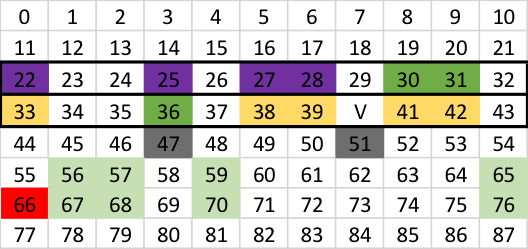
\includegraphics[width=0.6\textwidth]{figures/T66.png}
  \caption{Arrangement of agents at $T_{move_5''}$. }\label{fig:T66}
\end{figure}

\begin{figure}[H]
  \centering  
  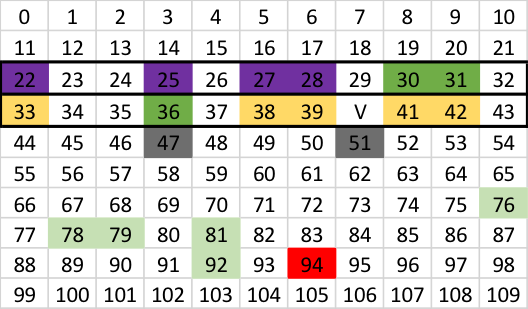
\includegraphics[width=0.6\textwidth]{figures/T94.png}
  \caption{Arrangement of agents at $T_{move_7''}$. }\label{fig:T94}
\end{figure}

We could know that the $CA$ moves back to its relative original position at $T_{notify\_7''}$. It would wait until next $T_{move}$ to inform its $Following\,Agent$ of $T_{trigger}$ and moves back with it.

\subsection{Overview of the Elimination}
After all the agents move back to where they are when the BV is triggered, we start the $Surrounding\,and\,Elimination$. We can destroy the BVs sequentially which is simple to execute but might in some case cost more time. In this way, because all the agents are aware of the positions of the new-formed BVs, so every time at most $d-1$ agents are sent to surround one of the BV and one agent is sent to destroy the BV and move on to decontaminate the second BV in a same way. Actually, this elimination strategy is the same as that in \cite{Alotaibi}. Or if we care most the execution time , we can destroy the BVs at one time. First we need to guard all the neighbouring nodes of the new formed BVs. In order to avoid collision and efficiently leverage the agents, we allocate different Destination Tables to all the agents in the array to inform them where should they should move in different situations (e.g., when the first agent in the exploring team is destroyed, then every agent except the first agent have a distinct destination, when the second agent is destroyed, then every agent except that agent destroyed have a distinct destination. More specifically, for a Chord Ring with half degree $d$, every agent in the array carries a $Destination\,Table$ with $d-1$ destinations. If we need more agents, then we will give their $Destination\,Table$ to the last agent in the shadowing group, when the elimination begins, it clones enough number of agents and give the $Destination\, Table$ to them. Before moving to its destination, the agent computes the shortest route from its own position to its destination using Dijkstra Algorithm. There are two kinds of agent in the Elimination phase: surrounding agents who are responsible for guarding the neighbouring nodes of the BVs and destroying agents who move to the BVs after all the neighbouring nodes are guarded. We want the BVs to be destroyed at one time, so it is important that the destroying agents move to the BVs at the same time and only after all the neighboring nodes are guarded by agents. In fact, if the destroying agents know the longest time $t_{longest}$ to move to the destination taken by all the agents (including the destroying agents and the surrounding agents), then they move to the last node prior to the destination and wait until $t_{longest}$ to move to the BVs together. So in the $Destination\,Tables$ for the destroying agents, we also add an item which is the $t_{longest}$. Now we introduce how to compute the shortest routes and how we design the $Destination\,Tables$. Note that we design $Destination\,Tables$ for all the agents and allocate them to the agents before the exploring phase begins.

\subsection{Destination Table and Elimination}
Supposing there are some BVs and agents in the chordal ring, it is obvious that the BV nodes are in the clockwise side of the agents. In order to use Dijkstra, first we need to map the chordal ring with BVs into a graph. We include nodes from the node containing the first agent to the node which is $d_k$ away from the last BV node, then delete the chords from the BV nodes to build the graph where we run Dijkstra Algorithm.
Here is an example how we built the graph for running Dijkstra Algorithm. Below we show the situation when the third agent in the exploring group is destroyed by the BV (see \ref{fig:D1}). Only the chords of the original BV node are shown. 
\begin{figure}[H]
  \centering  
  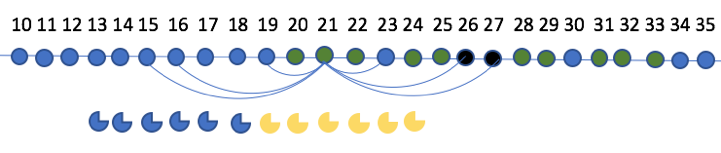
\includegraphics[width=0.6\textwidth]{figures/D1.png}
  \caption{Situation when the third agent in the exploring group is destroyed}\label{fig:D1}
\end{figure} 

The black node is the BV node while the green nodes need to be guarded. So in this case, we need 12 agents (10 surrounding agents and 2 destroying agents). 
We add nodes from 13 to 33 with their chords within this area and delete chords connected with the BV nodes to get the graph where we use Dijkstra Algorithm. Below is the graph we build. (see \ref{fig:D2}) For convenience, we show the all the nodes we included and the chords we delete.
\begin{figure}[H]
  \centering  
  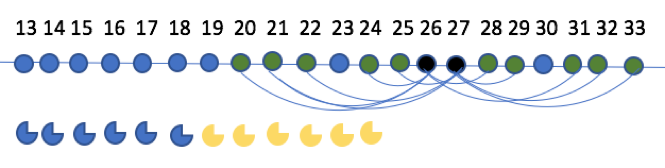
\includegraphics[width=0.6\textwidth]{figures/D2.png}
  \caption{The graph we build for Dijkstra Algorithm}\label{fig:D2}
\end{figure} 
Using the graph and Dijkstra Algorithm, we compute the routes from every agent to every node. Then we use enumeration to choose an allocation of every agents's destination satisfying: 
\begin{itemize}
\item 1) the maximum length of the route should be minimum. 
\item 2) after the allocation, in every needed position there should be exactly one agent.
\end{itemize}
After we get the optimal allocation, we record every agent's distinct destination and the position of the third agent in the exploring group in their $Destination\,Table$. Also, we add the length of the longest chord to every destroying agent.
More specifically, here we talk about the situation when the third agent in the exploring group is destroyed. For every agent, the information we compute would be in the third part of its $Destination\,Table$ recording the position of the third exploring agent (for example, it connects this agent through chord $x$), the destination it should move if the third exploring is destroyed. For a destroying agent, there should be another item recording the length of the longest route in this part.
Above we introduce how to design one part of $Destination\,Table$ of an agent, for every agent in chordal ring, it should hold a $Destination\,Table$ of $d-1$ parts, and every part contains 2 items (for surrounding agent) or 3 items (for destroying agent).
After the one of the agent is destroyed, the agent can check their $Destination\,Table$ to get the information of their destination. Then using Dijkstra Algorithm they can compute the shortest route separately and starts to move.

\section{Analysis and Comparing}
\subsection{Theorem and Proof}
\begin{theorem}
If the structure of a chordal ring is fixed, no mater where is the BV, the number of $Keep\,Moving$ agent is a constant.
\end{theorem}
\begin{proof}


Define: Going column, the column in which the agents keep going when an explorer encounters a virus.\\
Define: Stop column, the column in which the agents stop moving when an explorer encounters a virus.
We assume that the structure of the ring is $C_n(1, d_2, d_3,\dots, d_k)$, and there are d columns in the matrix which are $M={c_0,c_1,\dots, c_{d-1}}$\\
We assume the number of node where the original BV is V($P_V$), then it should in the column $c_{v\,mod\,d}$.\\
A column  is a stop column if and only if $\exists i,j\in [1,d]$, so that $(V+r_i)\,mod\,d=S$ or $(V-r_i)\,mod\,d=S$.\\
If the explorer encounters the virus at the position $P_{V+a}$ instead of $P_V$. Since $(V+r_i+a)\,mod\,d=(S+a)\,mod\,d$ or $(V-r_i+a)\,mod\,d=(S+a)\,mod\,d$, the column $c_{(S+a)\,mod\,d}$ should be a stop column.\\
In another word, if $c_S$ is a stop column when virus position is $P_V$, then $c_{(S+a)\,mod\,d}$ is a stop column when the virus position is $P_{V+a}$.\\
We assume we have two different stop columns $c_x$ and $c_y$ , when the black virus's position is $P_V$.  So when the black virus's position is $P_{V+a}$, the columns are $c_{(x+a)\,mod\,d}$ and $c_{(y+a)\,mod\,d}$. It is obviously that $\forall a$, if $x\neq y$, then $(x+a)\,mod\,d\neq(y+a)\,mod\,d$. That means we also have two different stop columns. So that the number of stop column does not decrease, which means that given a fixed chordal ring $C$ and the number of agent keeping moving when the BV is in V (V can be any position), then the number of agent keeping moving when the BV is in other position does not decrease.\\
Let us assume that the number of agents keeping moving in different case when the longest chord remains the same is different and donates the minimum number of going columns among them by $N_{minimum}$ while the maximum number of going columns among them by $N_{maximum}$, then according to our conclusion $N_{minimum}\geq N_{maximum}$, which means that $N_{minimum}= N_{maximum}$ . In another word, the number of agents keeping moving is a constant when the structure of the chordal ring is fixed. 
\end{proof}

%The second theorem is reserved for proving the number of agents needed in different strategies in elimination
 
\subsection{Analysis and Comparing}

\noindent{\bf Time cost analysis and comparing}

We only consider the situation when n (the number of nodes of the chordal ring) is much larger than $d_k$, and since the time cost in the elimination phase is $O(1)$.  Finally, we compute the TWT of both protocols to present a more fair comparison.
Let us assume that the total number of moves is $M$, then the worst case costing the most time is when the BV is located at any nodes with number from $n-d_k+1$ to $n-1$ and the first agent (anticlockwise) is in the node with the number $n-d_k$. In this case, it cost $M=\left \lfloor \frac{n}{d_k}-1\right \rfloor$ moves and 4$M$ units of time (4$M=4\times \left \lfloor \frac{n}{d_k}-1\right \rfloor$) to finish the exploring phase. 
In \cite{Alotaibi}, she give the number of move in three case.
\begin{itemize}
\item 1) In double loops the upper bound of moves is $4n-7$.
\item 2) In the triple loops, she discusses two classes of chordal ring: $C_n(1,p,k)$ and $C_n(1,d_k-1,d_k)$.In the first case, the number of moves needed is $5n-6d_k+22$ while in the second case, a maximum of $5n-7d_k+22$ moves are needed.
\item 3) In the consecutive-chordal rings, a maximum of $(d_k+2)n-2d_k-3$ moves are needed.
\end{itemize}
Since in the sequential strategy, agents do not need to wait so the time cost is equal to the number of moves. And it is obvious that our protocol is much faster than the sequential strategy. But since we use much more agents, so in order to gain a fair comparison, now we compute TWT of both protocol.
In the exploring phase, we use $2d_k$ agents, so the TWT of our protocol is $8n-8d_k$. In the exploring phase of the sequential strategy, it need at least 2 agent to explore and some other shadow agents to guard the explored nodes but the number of shadow depends on the structure of the chordal ring so now we ignore them. Now we compute TWT of the sequential strategy.
\begin{itemize}
\item 1)In double loops the upper TWT is $8n-14$
\item 2)The TWT in chordal ring $C_n(1,p,d_k)$ is $10n-6d_k+44$ and in chordal ring $C_n(1,d_k-1,d_k)$ is $10n-14d_k+44$.
\item 3)The TWT in consecutive-chordal rings is $2(d_k+2)n-4d_k-6$.
\end{itemize}
It is obvious that when $d_k\geq 2$, our protocol is faster in first case; when $d_k\leq \frac{1}{3}n+7$,our protocol is faster in the second case (both $C_n(1,p,k)$ and $C_n(1,d_k-1,d_k)$); when $d>2-\frac{1}{n+2}$, our protocol is faster in the third case.

\noindent{\bf Calamity Analysis}
Casualty is the number of agents destroyed by the BV. In chordal ring $C_n(1, d_2,\dots, d_k)$, the worst case is that the first agent in the exploring group is destroyed by a BV and the clones of it spread to all its neighbouring nodes. The casualties in this case are $d_k+1$ because another $d_k$ nodes are guarded by agents while in sequential case, the casualties are $2d_k$. So in terms of casualty, our protocol is better than the sequential strategy.

%Following part are reserved for analysis for different strategy in elimination: including proposing function to calculate the exact cost of different strategies...






%%%%%%%%%%%%%%%%%%%%%%%%%%%
\chapter {Parallel Black Virus Decontamination in Arbitrary Graph}
\label{TL}
%%%%%%%%%%%%%%%%%%%%%%%%%%%

\section{Introduction}
In \cite{Cai}, Cai proposes two exploration strategies: Greedy Exploration and Threshold Exploration, both spread optimal and total number of agents asymptotical optimal. Since these strategies are sequential, they are time consuming($O(\Delta n^2)$).  In order to explore the graph parallelly, we propose two different strategies: \\
(1) Flood Strategy\\
(2) Castle First Strategy\\
The general idea of the Flood Strategy is simple, supposing that an agent resides in node $v$, and it has $i$ neighbours excepted to be explored, then it simply clones $v$ agents and send them to its neighbours. In Castle First Strategy, we build castles which is a node or the combination of several nodes(rules are introduced later), the exploration phase can be viewed as the combination of many smaller scale exploration in the graph which begins with the location of one of the exploring group and ends with one of the unexplored castles. After all the castles are explored, all the nodes in the graph are explored. The general exploring strategy for these two strategies is based on the one described in Chapter 3 which consists of performing a {\em Shadowed Exploration} phase to locate the BV, followed by a {\em Surrounding and Elimination} phase to eliminate the cloned BVs. 

Strategy {\em Flood}  is time optimal with the cost of a great number of agents while strategy {\em Castle First} comes to a compromise between the strategy {\em Flood} and the sequential strategies: it employ much less agents than the strategy {\em Flood} while cost much less time than the sequential strategies. 

In the arbitrary graph, we assume that any node does not disconnect the graph.

\section{Parallel Strategies for BV Decontamination in Arbitrary Graph}
\subsection{Flood Strategy}
\noindent{\bf Initialization}
In this strategy, all the agents are endowed with 3-hop visibility. Also, all the agents do not need to remember the routes they pass. Finally, in this strategy, we use an important ability of agents which is clone. As we introduced in Chapter 2, clone means that a agent is endowed with the capacity to generate one or more agent. 

We use the Dijkstra Algorithm to compute the shortest route step for every node and write them on the white board on each node, so for each node, there should be a number (Shortest Route Number) recording the number of steps of the shortest route from the homebase to it. Let us denote by $v_{SRN}$ the Shortest Route Number of node $v$, and nodes ${v_1, \ldots, v_i}$ are neighbours of node $v$ assuming that $v$ has $i$ neighbours. Then edges connecting node $v$ and its neighbours are $e(v, v_1), \ldots, e(v, v_i)$. We write the $v_{SRN}$ to the end of these edges (the end connecting to its neighbours), so when an agent resides in any node from $v_1$ to $v_i$, it can see the Shortest Route Number of node v because of the local visibility. (For example, see Fig\ref{fig:Arbi1}) 

\begin{figure}[H]
  \centering  
  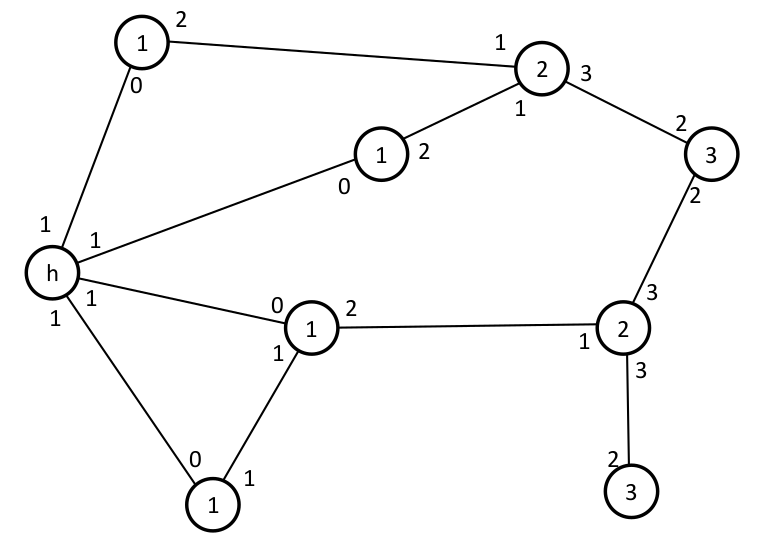
\includegraphics[width=3in]{figures/Arbi1.png}
  \caption{Initialization of the graph}\label{fig:Arbi1}
\end{figure}

\noindent{\bf Exploration Phase}
All the agents in this strategy follow the same rules in the exploration phase.

Rules for agents in the exploration phase:
Let us denote by $SNR$ the Shortest Route Number.
\begin{enumerate}
\item Agents can only move from node with lower $SNR$ to node with higher $SNR$.
\item Assuming that there are $x$ agents residing in node $v$, and the next destination(s) are $\{v_1,\ldots, v_i\}$. 

        if $x\geq i+1$, then $i$ agents move to the destinations respectively while one agent stays in node $v$ to guard $v$ at $T_i$. If one of agents is destroyed, the Elimination phase begins; if none of the agents is destroyed, the left $x-(i+1)+1(the one who guards the node $v$)$ agents evenly move to the destinations at $T_{i+1}$. 
        if $x< i+1$, then one of the agents residing in node $v$ clones $i+1-x$ agents, and these $i$ agents move to all the neighbours at $T_i$. If one of the agents is destroyed, the Elimination phase begins; if none of the agents is destroyed, the agent guarding the node $v$ randomly moves to one neighbour with $SNR$ equal to $a+1$ at $T_{i+1}$.
\item If an agent resides in a node (assuming its $SNR$ is $a$) without any neighbour whose $SNR$ equal to $a+1$, then it simply stays there.
 
        Since all the action of agents happen after they meet each other at the same node, they can communicate with each other and make sure that all their routes do not conflict.
\end{enumerate}
An example of how the agents move is showed in Fig\ref{fig:Arbiflood}
\begin{figure} [H]
  \centering 
  \subfigure[$T_1$]{ 
    \label{fig:Arbiflood1:a} %% label for first subfigure 
    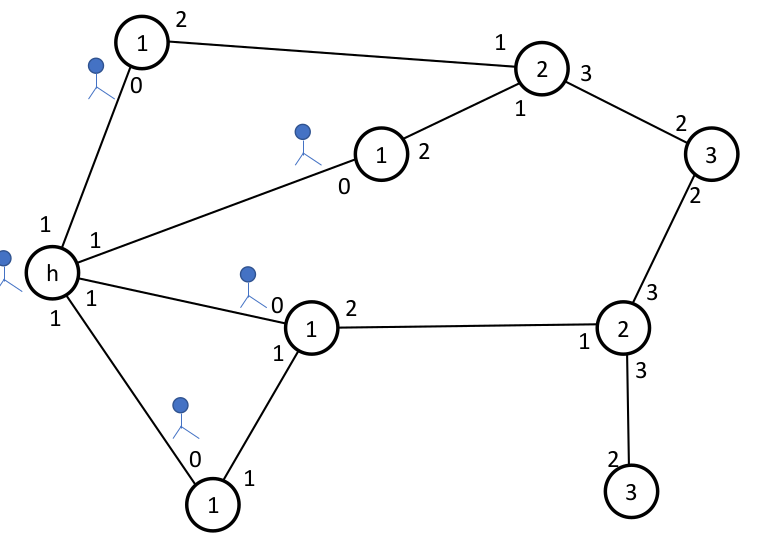
\includegraphics[width=2.5in]{figures/Arbiflood1.png}} 
%  \hspace{1in} 
  \subfigure[$T_2$]{ 
    \label{fig:Arbiflood2:b} %% label for second subfigure 
    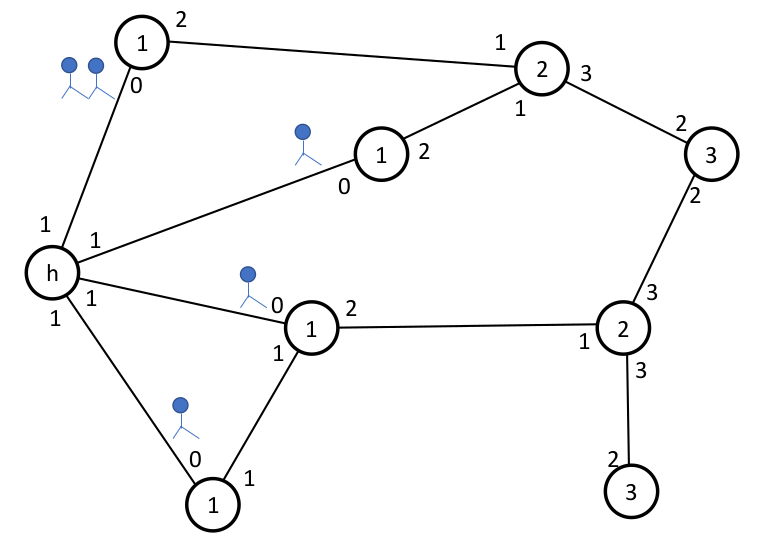
\includegraphics[width=2.5in]{figures/Arbiflood2.png}}
    \hspace{1in} 
  \subfigure[$T_3$]{ 
    \label{fig:Arbiflood3:c} %% label for second subfigure 
    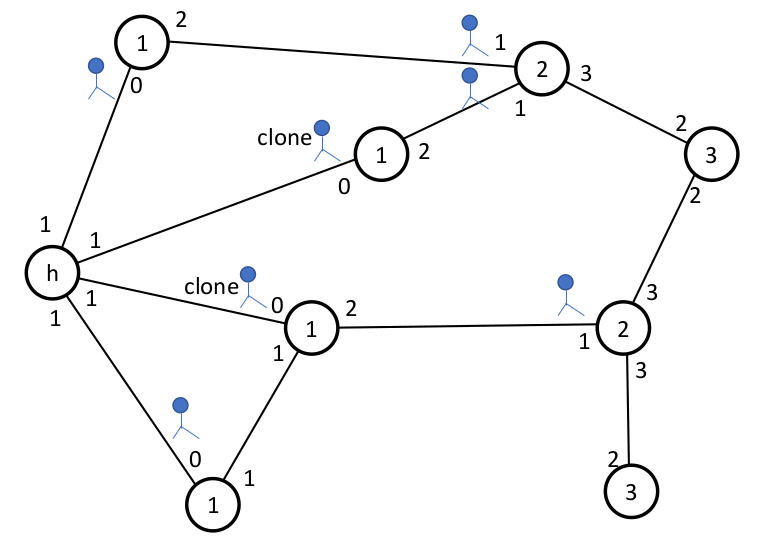
\includegraphics[width=2.5in]{figures/Arbiflood3.png}}
%      \hspace{1in} 
  \subfigure[$T_4$]{ 
    \label{fig:Arbiflood4:d} %% label for second subfigure 
    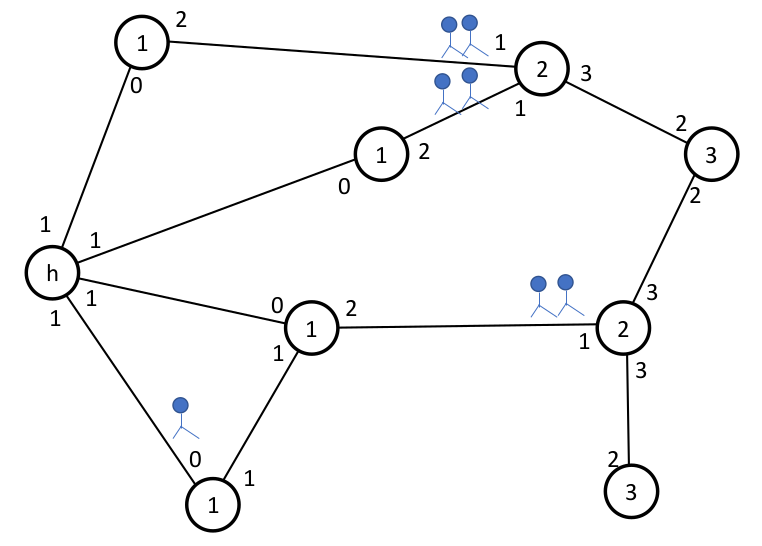
\includegraphics[width=2.5in]{figures/Arbiflood4.png}}
      \hspace{1in} 
  \subfigure[$T_5$]{ 
    \label{fig:Arbiflood5:e} %% label for second subfigure 
    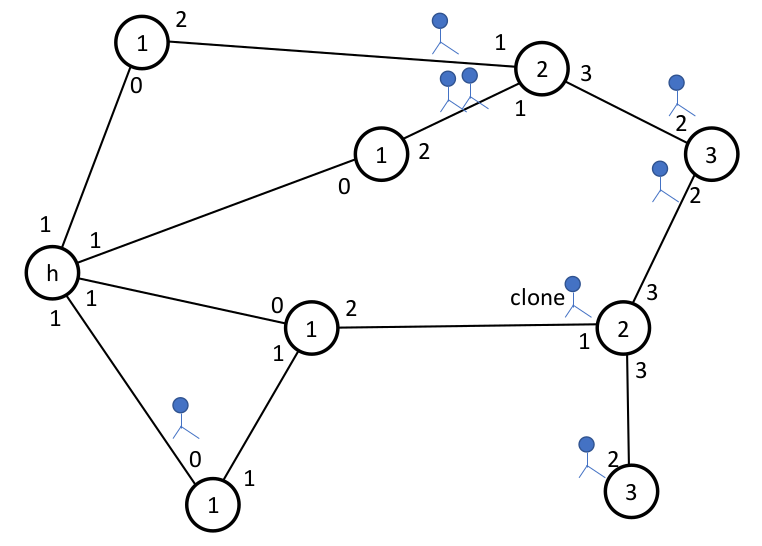
\includegraphics[width=2.5in]{figures/Arbiflood5.png}}
     \subfigure[$T_6$]{ 
    \label{fig:Arbiflood6:e} %% label for second subfigure 
    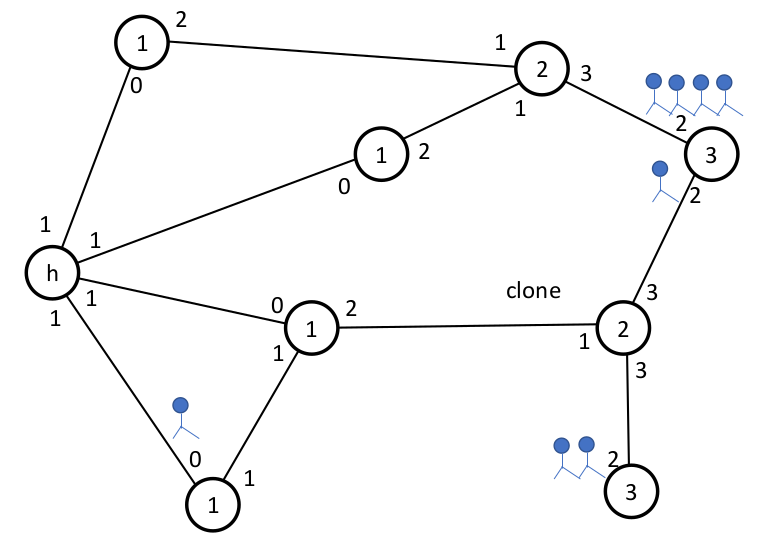
\includegraphics[width=2.5in]{figures/Arbiflood6.png}}
  \caption{An example of how the agents move in the Flood Strategy} 
  \label{fig:Arbiflood} %% label for entire figure 
\end{figure}

\noindent{\bf Elimination Phase}
Let us assume that the node where the original BV resides is $v$ with $SNR$ equal to $a$ and it is triggered at $T_i$. Then at this time, the clones spread to all neighbours of node $v$ with $SNR$ equal to $a+1$ and survive while leaving node $v$ clean (no agent and no BV) and let us denote by $v_{BV}$s all these BV nodes.  

Now we introduce how agents residing in different positions move in the Elimination phase.
\begin{enumerate}

\item Rule 1: We call agents residing in the these $v_{BV}$s' neighbours with $SNR$ equal to $a$ the Witness Agent, and these Witness Agent can easily realize whether or not node $v$ is the place where the original BV resides. For example, since they have 3-hop visibility, so if they see that one of their ``2-distance" neighbours (say node $v'$) does not contains an agent but some neighbours of node $v'$ contain agents, then they can know that the original BV resides in node $v$. If the Witness Agents realize the existence of BV at $T_1$, then they simply stop cloning and moving. 

\item Rule 2: For all of the agents residing in node $v$'s neighbours with $SNR$ equal to $a-1$ (say the number of them is $y$), they receive clones and realize the location of the BV and would move to $v$ at $T_{i+1}$. Let us denote by $z$ the number of $v$'s neighbours with $SNR$ equal to $a+1$, then if $y< z+1$, one of the agents residing in node $v$ should clone another $z+1-y$ agents and then $z$ agents move to $v$'s neighbours with $SNR$ equal to $a+1$ at $T_{i+2}$.
\end{enumerate}

See Fig\ref{fig:Arbiflood}. For convenience of description, we give every node in the graph a distinct ID from 1 to 13. As shown in the picture, when the BV is triggered, the clones spread to all neighbours of node 3, and node 4 and 5 become new BV node while nodes 1, 2 and 12 destroy a clone respectively and realize that the original BV resides in node 3.

\begin{figure}[H]
  \centering  
  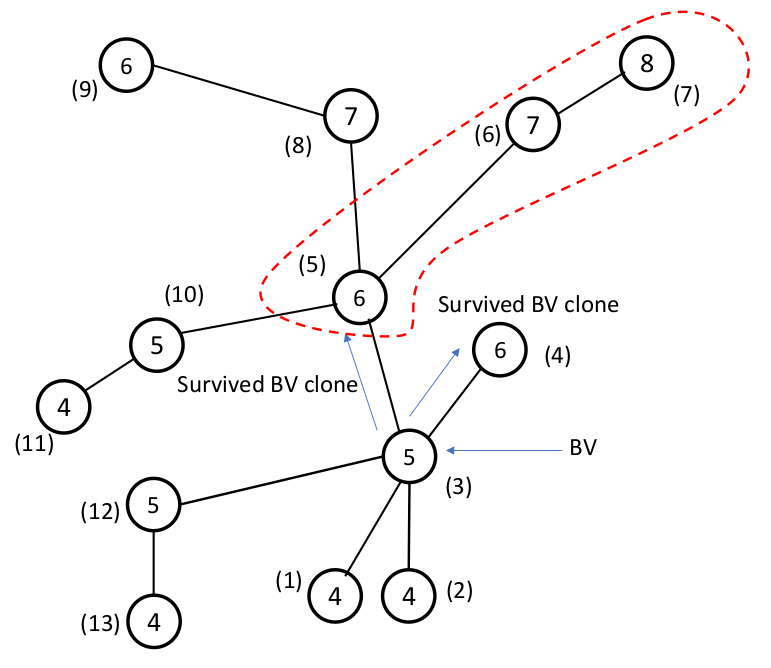
\includegraphics[width=3in]{figures/Arbi3.png}
  \caption{An possible situation when the BV is detected}\label{fig:Arbi3}
\end{figure} 

In Fig.\ref{fig:Arbi3}, node 10 is a Witness Agent and because of the 3-hop visibility, it can ``see" that there is no agent residing in node 3 but there are agents residing in node 3's neighbours which are node 1 and node 2. By this way, it knows that the original BV resides in node 3 and it stop moving and cloning.

For convenience, let us denote by $a$ the $SNR$ of the original BV node. Since in our assumption, any node does not disconnect the graph, so the following situation would not happen:
\begin{enumerate}
\item All the higher $SNR$ neighbours of the new formed BVs have only one neighbour with lower $SNR$ and it is the BV node, \item Some of the neighbours of the new formed BVs have at least one neighbour with lower $SNR$ except their BV neighbour while some of the neighbours of the new formed BVs have only one neighbour with lower $SNR$.
\end{enumerate}
For example, see \ref{fig:Arbi3}. The situation shown in the red circle is the case when the node 5 disconnect the graph.The new formed BVs has two higher $SNR$ neighbours which are nodes 8 and 6. Node 6 has only one neighbour with lower $SNR$ and it is the BV node. Assuming the BV is triggered at $T_i$, then at $T_{i+2}$, all the BVs are decontaminated except one: the BV clone spreading to node 6, so we can only employ an agent to move to node 6, then to node 7 and the BV is permanently destroyed and we do not want it to happen.

With our assumption, all the higher $SNR$ neighbours of the new formed BVs have at least one neighbour with lower $SNR$ except their BV neighbour.  Since agents who do not know the existence of the BV keep moving and at $T_{i+2}$, they would move to occupy nodes with $SNR$ equal to 7 which means all the neighbours of the new formed BV are guarded. In this way, all the BVs are permanently destroyed at $T_{i+2}$.

               
\subsection{Castle First Strategy}
\noindent{\bf Introduction}
In the Castle First Strategy, all the agents have only the local visibility. But the leader agent in each exploration group have the map of the graph in its memory. Also, the leader agents are endowed with the ability of clone.

In the Castle First Strategy, we built some castles based on the graph with $SNR$. More than one group of agents are sent to explore the graph respectively. Their exploration of the graph are separated into many ``sub-exploration"s and each ``sub-exploration" begins with where the agents are and ends with a new unexplored castle. The map of the graph with all the castles being pointing out is recorded on the whiteboard on nodes with more than two neighbours (the intersection) so when agents move across these nodes, they can update the information on the whiteboard (for example, changing the state of some castles into explored) or update its own memory. When agents cannot find an unexplored castle in the graph, then they terminate. 

\noindent{\bf Initialization}
Based on the graph marked $SNR$ for every node, we built another graph called ``Castle Graph". 
We now give the definition of ``Castle":
\begin{enumerate}
\item Case 1: Node who has one neighbour is a ``Castle".
\item Case 2: If a node has at least one neighbour with the same $SNR$ as it, then the combination of them is a castle. If different castles have at least one common node, then we merge them into a bigger castle;
\item Case 3: If a node has more than two neighbours with lower $SNR$ than itself, than this node is a castle.
\end{enumerate}

Some examples of castles are shown in Fig\ref{fig:CastleExample}
\begin{figure}[H]
  \centering  
  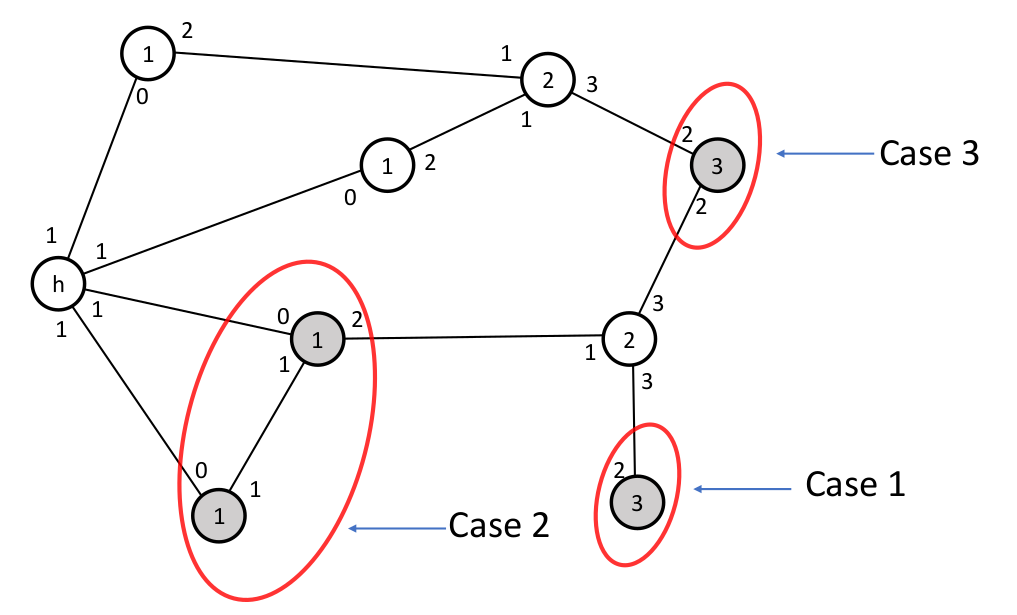
\includegraphics[width=3.5in]{figures/CastleExample.png}
  \caption{Examples of Castles}\label{fig:CastleExample}
\end{figure} 

After the processing, we have a new graph called ``Castle Graph" and this graph is presented on the whiteboard on the nodes which have more than two neighbours, so when the agent reaches this node, it can read the graph to update its own information or using its own information to update the ``Castle Graph". 

\noindent{\bf Exploration Phase}
There are two principle in the exploration phase for the agents:
\begin{enumerate}
\item when agents move in an unexplored area, they should strictly move from node with smaller $SNR$ to node with bigger $SNR$ and should follow the ``casual walk" while when move in an explored area, they can move in opposite (from bigger $SNR$ to smaller $SNR$) and when the agents move in this area, they are allowed not to follow the ``casual walk" (for example, when they plan to explore node $v$ from node $u$, the LA can directly move to node $v$ when node $v$ is in the explored area) which is called ``normal walk".
\item The castle selected to be the destination of the ``sub exploration" should meet the follow the following requirement: assuming that the $SNR$ of the destination castle is $a$ and the node from where the agents start the ``sub exploration" is $v$  , then for every node with $SNR$ equal to $a-1$ connected to the castle, there should be a route from $v$ to these nodes and no castle(s) which are not explored (the castles can be in the state of ``under exploring" or ``explored") existing on these routes. In another word, when the agents move from $v$ to these node, except the destination castle, they do not need to ``attack" other castles. 
\end{enumerate}  

There are two kind of agents in this strategy: Leader Agent (LA) and Shadow Agent(SA) and the LA has the map of the whole graph in its mind. When more agents are needed, the LA would clone the agents. At the beginning of the exploration phase, the LAs are in the homebase, so they respectively pick a castle to be the destination of the their first ``sub exploration" and since they have the map of the graph, they can compute a shortest route for the ``sub exploration" and then are sent randomly from the homebase. 

The agents are divided into three status: Finding Castle, Attacking Castle and Waiting in Line. 

Initially, the status of all agent group are ``Finding Castle".In a agent group with the status of ``Finding Castle", if the LA in that agent group can find an available castle, then the status of this group changes into ``Attacking castle". Unless the agent group realizing the existence of BV, the status of the agent group changes into ``Finding Castle" at the end; if the LA in that agent group cannot find an available castle but there are still castle unexplored in the graph, then the status of this group changes into ``Waiting in line". Unless the agent group realizing the existence of BV, the status of agent group changes into ``Finding Castle" at the end. 

(1) From ``Finding Castle" to ``Attacking Castle"

When the status of an agent group changes into ``Attacking Castle", the LA in this exploring group updates the information on the whiteboard on the node along its route to that castle. On the way to their destination (the castle), the agents follow the ``casual walk" in the unexplored area and ``normal walk" in the explored area: when exploring the node $u$ from the node $v$, one of the SAs moves to node $u$, when the node $u$ is safe, it returns to node $v$ and moves to the node $u$ with the LA and the other SAs; when the node $u$ contains a BV, then the LA knows the existence of the BV by receiving the clone of the BV.   

Along the route to the group's destination, the LA updates the information (changing the state of the destination castle to be under explored) of the intersections and also read information from them, if it finds that the destination castle of its ``sub exploration" has been explored or under exploring (for example, when it read the information from the whiteboard of the intersection on the route and it shows that that destination castle's state is ``explored" or ``under exploring"), then the status of its group changes into ``Finding Castle" again. If not, then this group reach one of the destination castle's lower $SNR$ neighbour and the LA starts to arrange the SAs to guard all the lower $SNR$ neighbour(s) of the castle. 

After the arrangement of the SAs, it should be ensured that all the lower $SNR$ neighbours of the castle are guarded and assuming that there are $x$ nodes in the castle $\{castle\_0, \ldots, castle\_x\}$, another $x$ SAs (Attacking Agent) should move to these $x$ nodes at the same time. In order to do that, we propose one possible strategy for the LA to place the SAs: assuming that the sequence of the nodes which should be guarded is $\{node\_0, \ldots, node\_y\}$, and $node\_i$ is the last node in the sequence connected to $castle\_k$ where $0\leq i\leq y$, $0\leq k\leq x$, then the LA should place two agents in $node\_i$ while place one agent in the other nodes when it moves in sequence to place the SAs. Also, the LA knows the time when it finishes the arrangement of the last agent(s), then it should inform the agents the exact time to move to the castle nodes and permanently destroy the BVs.

When one agent group starts to surround the castle, by which we mean that the LA has placed SAs in at least one lower $SNR$ of the castle, it is possible that another agent group has started to surround the castle (even the LA updates the information when it moves, still the consistency of all the information cannot be guaranteed). The LA of an agent group realize this by meeting an SA not from its group when it arranges the SAs to guard the lower $SNR$ neighbours of the castle. We prefer to avoid conflict when two agent group explore one castle (SAs from two different agent group move to the castle nodes). The LA can compute the time when the arrangement is finished and record it on a timestamp, so when the LA places the SAs, it leaves timestamp with these SAs. By doing this, every SA from one agent group guarding the castle hold a timestamp recording when does the arrangement end and if a LA meet a SA from other agent group with a earlier timestamp, it move back to collect the SAs in its group that have been placed and the status of this agent group turn into ``Finding Castle". 

When the arrangement is done, the LA resides in the last node needing guarded and in the next unit of time, all the Attacking Agents move to the castle nodes. Note that at this time, if there is a BV in the castle, not all the guarding agents can receive a BV clone. As shown in Fig\ref{fig:MultiCastleNode}, when the BV is triggered, except the castle nodes, only the guarding agents 1 and 2 receive the clones.
\begin{figure}[H]
\centering  
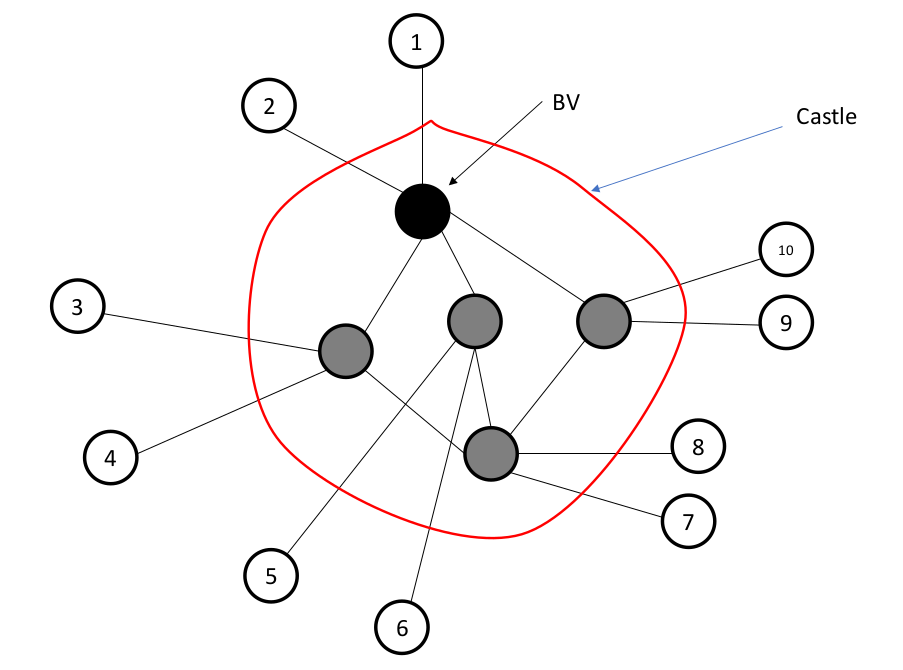
\includegraphics[width=3.5in]{figures/MultiCastleNode.png}
\caption{An example shows that if there is a BV in the castle, in some cases not all the guarding agents can receive a BV clone}\label{fig:MultiCastleNode}
\end{figure} 

So after the ``attacking" by the ``Attacking agent", the LA should execute the ``Double Patrol". Now we introduce what is the ``Double Patrol".
\begin{enumerate}
\item 
The LA first computes a route to traverse all the castle nodes, (say the route is $castle\_0\rightarrow castle\_1 \rightarrow\ldots, castle\_x$ assuming that there are $x$ nodes in the castle). In this first ``patrol", the LA first leaves a flag saying ``First Patrol" and then moves to one castle node, it tells the SA residing in that castle node to collect the SAs residing in all its lower $SNR$ neighbours and finally move to that castle node with all these collecting SAs. Also, when the SA collects the ones residing in the lower $SNR$ neighbours, it places a flag on that neighbour node saying ``First Patrol". After the LA traverses all the castle nodes, it can easily know whether there is a BV in the castle: if there is no BV in the castle, then there should be one agent residing in every castle node, if not, then there is a BV and the clones of it have move to all higher $SNR$ neighbours of this node. If the LA realizes that there is a BV, then the Elimination Phase ends, if not, then the LA move back to the first castle node with the route $castle\_0\rightarrow castle\_1 \rightarrow\ldots, castle\_x$ and when it moves to that castle node, it should wait until all the guarding agents have been collected and move to the next castle node. When the LA move back to the first castle node, the ``First Patrol" finishes. See Fig.\ref{fig:FirstPatrol}
\begin{figure} [H]
  \centering 
  \subfigure[$T_a$]{ 
    \label{fig:FirstPatrol1:a} %% label for first subfigure 
    \includegraphics[width=2.5in]{figures/FirstPatrol1.png}} 
%  \hspace{1in} 
  \subfigure[$T_{a+1}$]{ 
    \label{fig:FirstPatrol2:b} %% label for second subfigure 
    \includegraphics[width=2.5in]{figures/FirstPatrol2.png}}
    \hspace{1in} 
  \subfigure[$T_{a+2}$]{ 
    \label{fig:FirstPatrol3:c} %% label for second subfigure 
    \includegraphics[width=2.5in]{figures/FirstPatrol3.png}}
%      \hspace{1in} 
  \subfigure[$T_{a+3}$]{ 
    \label{fig:FirstPatrol4:d} %% label for second subfigure 
    \includegraphics[width=2.5in]{figures/FirstPatrol4.png}}
      \hspace{1in} 
  \subfigure[$T_{a+4}$]{ 
    \label{fig:FirstPatrol5:e} %% label for second subfigure 
    \includegraphics[width=2.5in]{figures/FirstPatrol5.png}}
     \subfigure[$T_{a+5}$]{ 
    \label{fig:FirstPatrol6:f} %% label for second subfigure 
    \includegraphics[width=2.5in]{figures/FirstPatrol6.png}}
     \subfigure[$T_{a+6}$]{ 
    \label{fig:FirstPatrol7:g} %% label for first subfigure 
    \includegraphics[width=2.5in]{figures/FirstPatrol7.png}} 
%  \hspace{1in} 
  \subfigure[$T_{a+7}$]{ 
    \label{fig:FirstPatrol8:h} %% label for second subfigure 
    \includegraphics[width=2.5in]{figures/FirstPatrol8.png}}
    \hspace{1in} 
  \subfigure[$T_{a+8}$]{ 
    \label{fig:FirstPatrol9:i} %% label for second subfigure 
    \includegraphics[width=2.5in]{figures/FirstPatrol9.png}}
%      \hspace{1in} 
  \subfigure[$T_{a+9}$]{ 
    \label{fig:FirstPatrol10:j} %% label for second subfigure 
    \includegraphics[width=2.5in]{figures/FirstPatrol10.png}}
      \hspace{1in} 
  \subfigure[$T_{a+10}$]{ 
    \label{fig:FirstPatrol11:k} %% label for second subfigure 
    \includegraphics[width=2.5in]{figures/FirstPatrol11.png}}
  \caption{An example of  ``FirstPatrol"} 
  \label{fig:Arbiflood} %% label for entire figure 
\end{figure}

\item 
After the first patrol, the LA knows that if there is a BV. If there is, then the Exploration phase ends, and the Elimination phase starts. If there is not, then the ``Second Patrol" starts. In the ``Second Patrol" the LA moves along the route as it does in the ``First Patrol" which is $castle\_0\rightarrow castle\_1 \rightarrow\ldots, castle\_x$. Also it collects all the SAs in the castle node it passes by and updates the information on the whiteboard on the castle node saying that the castle is explored. 
\end{enumerate}  
After the ``Second Patrol", the status of this agent group changes into ``Finding Castle". 


(2) From ``Finding Castle" to ``Waiting in Line"

When the status of the agent group changes into ``Waiting in Line", then it means that the  LA in that agent group cannot find an available castle but there are still castle unexplored in the graph. At this time, the LA  randomly chooses an  castle marked ``under exploring" and move there with its agent group. When the agent group arrives one of the lower $SNR$ neighbours of that castle we call them the ``Guarding Node", three situations may happen:
\begin{enumerate}
\item Case 1: The agent group arrives there finding that no SA(s) and no flag in that  Guarding Node. In this situation, the agent group who is excepted to attack this castle may not yet arrive this castle or does not finish the arrangement of the SAs. Then the agent group should wait at that Guarding Node until there is an SA and follows the instruction in case 2.

\item Case 2: The agent group arrives there finding at least one SA. In this situation, it means that the agent group who is excepted to attack the castle has finished arranging the SAs but has not finished the ``First Patrol". So this agent group stays with the SA until the SA is called by another SA and move into the castle. After moving into the castle node, the agent group should wait the LA of the agent group who is attacking the castle to move to this castle node again because at this time the LA would update the situation in the castle: whether there is a BV or not. If there is a BV in the castle, then agent group who is waiting in the castle node ends its exploration phase and start the elimination phase; If not, then the status of this agent group changes into ``Finding Castle".

\item Case 3:The agent group arrives there there finding there is a flag on that guarding node. It means that the LA of the agent group who is excepted to attack the castle is doing the ``First Patrol" or has finished the first ``First Patrol", or is doing the second ``Second Patrol". In this situation, the agent group moves into the castle node which is connected to the guarding node it arrives and wait the LA of the agent group who is attacking the castle to move to this castle node again. As in the case 2, this agent group can know the if there is a BV in the castle and follows the same instruction as in the case 2: if there is a BV, then the agent group starts the elimination phase, if not, the status of it changes into ``Finding Castle".

\end{enumerate}


\noindent{\bf Eliminaiotn Phase}

When the BV is triggered, then the location of the BV can be in a castle or outside the castle. In both situation, the lower $SNR$ neighbours of the BV node or the castle containing the BV have been guarded by the agents. In another word, when the BV is triggered, only the clones spreading to the higher $SNR$ neighbours (say that the number of them is $y$) survive and their locations are exposed. Also, the locations of all the neighbours of these new formed BVs are exposed. 

So the LA computes the routes from where it resides to all the nodes needing guarded including the lower $SNR$ neighbours and the higher $SNR$ neighbours(Surrounding Nodes). When the location of the original BV is outside the castle, then all the SAs stays with the LA, so the LA simply sends the SAs to these Surrounding Nodes. When the original BV is in the castle, then after the  ``Double Patrol", the LA knows the location of the original BV so it computes the routes from where it resides to all the Surrounding Nodes and sent the SAs to them (note that all the SAs are with the LA after the  ``Double Patrol"). Note that in our assumption that any node in the graph does not disconnect the graph, there is always another route to reach the surrounding node  except bypassing the new formed BV nodes. Assuming that there are $x$ higher $SNR$ neighbours of the original BV, then finally, the LA sends another $x$ to the new formed BV nodes and permanently destroy the BVs.









 
%%%%%%%%%%%%%%%%%%%%%%%%%%%
\chapter {General Chordal Rings}
\label{GL}
%%%%%%%%%%%%%%%%%%%%%%%%%%%
Now that we have investigated the problem of disinfecting a network from a  \bv   in   special  classes of chordal rings, we will discuss the problem in general chordal rings, regardless of chords structure.  


The solution  we propose is based on the  idea described for the general chordal ring in Chapter \ref{PM}, and has already been explained throughout this thesis. It involves an exploring phase, followed by a surrounding phase. Our protocol is based on a general surrounding method that can be applied to any chordal ring structure, regardless of the number or distance of chords. It must be noted that the move-cost for this method is not optimal.

 


 \section{Exploring and Shadowing}
%The main goal of this phase is to determine the location of the original \bv since the location of the \bv is unknown a priori. This process is done by the  exploring team: $LEA$,$EA$, and shadow agent(s) $SA$. 
%Finding the node in which the \bv resides implies creating more \bvs in some cases, destroying $EA$, and clearing that node. As we mentioned before, the technique used in this phase is the {\em safe exploration}.
%\begin{comment}
%Starting from a random node, \hb, $v_0$, the leader and the exploration agent explore the chordal ring
%node by node along the outer ring  (i.e., using only $d_1=1$) in the clockwise direction.  $EA$ moves to the next node $v_{1}$ while $LEA$ waits at $v_{0}$; if $EA$ returns back to its leader, then $v_{1}$ is not a \bv and they both move to $v_{1}$ and so on. However, if $LEA$ receives a \bv instead of $EA$, then the location of the original \bv is detected. 
%\end{comment}
%In order maintain monotonicity, $SH$s are deployed. The deployment of $SH$s starts when $LEA$ and $EA$ have explored at least $d_2$ nodes. 
%\begin{comment}
%In other words, if  $C_n( d_1=1, d_{2}, ..., d_{m})$, and the exploring team currently exploring node $v_j$
%and $\left\vert{S_{area}}\right\vert \ge d_2$, at least one $SA$ is deployed and the number of $SA$s increases as many as the neighbours of the current explored node in the safe area, the number of $SH$s $=|N_{ex}(v_j)|-1$.
%Once $EA$ arrives to the \bv location, it is destroyed, $LEA$ receives a $BV$ instead of EA, that node is cleared, new \bvs are located at all the unprotected(unexplored) neighbours of the original $BV$.
%
%  Since we have a monotone protocol, the explored nodes  in ($S_{area}$) should be protected from potential recontamination. As we mentioned before, the exploring team ($LEA$,$EA$) are moving in clockwise direction along the outer ring, but when they reach a certain node ($v_{n-d_m}$), the possibility of infecting explored node(s) increases; thus, in addition to $SH$s at counter clockwise neighbours, $SH$s are needed at the clockwise neighbours . As we have mentioned before, the area in which the recontamination possibility increases is called danger area  $D_{area}$ where $v_{n-d_m} \leq D_{area}\leq v_{n-1} $.
%\end{comment}
% 
%
%  \begin{center}
%\fbox{
%\begin{minipage}{6 cm}
%{\sc  Exploring and Shadowing}
%  \begin{tabbing}
%  Age\= nts $EA $ and $$LEA$$ at safe node  $v_i$.\\
%\\
% - Compute  $N_{ex}(v_{i+1})$ \\
% - For each $q \in N_{ex}(v_{i+1})$ \\
% \tab  $SH$\ is deployed \\
% - $EA$ moves to $v_{i+1}$\\ \\
% If $EA$ returns back to $v_{i}$\\
% \tab $LEA$ and $EA$ move to $v_{i+1}$\\
% Else (i.e., $BV$ moves to $v_{i}$)\\
%\tab $EA$ is destroyed\\
% \tab $|BV|=N_{un}(v_i)$
%  \end{tabbing}
%\end{minipage}
%}
%\end{center}
%

 The   phase is  described in detail in Chapter \ref{PM}. The following are our observations in general chordal ring structures:

\begin{theorem}

In any  chordal ring $C_n=\{1,d_2,d_3,...,d_m\}$, in the worst case scenario, the \bv is detected in $((2+m)n-2m-3)$ moves.

\end{theorem}
\begin{proof}
The worst case scenario regarding the number of moves required occurs when the \bv  is located at node ($v_{n-1}$) after exploring   $n-1$ nodes.  
 The complexity of this case would be $3n-5$ for the movement of $LEA$ and $EA$, $(\sum\limits_{i=2}^m n-1-d_i)$ for the movement of $SH$s to counter-clockwise neighbours and $(\sum\limits_{i=2}^m d_i-1)$ for $SH$s to clockwise neighbours. 

 In this case, the \bv triggers no new \bvs since all of the neighbouring nodes are occupied by $SH$s, ($2m-1$) $SH$s. This case is considered the worst case scenario in terms of calculating the number of moves, but the best case in terms of cleaning and surrounding agents.
\end{proof}

 
\begin{theorem}

In any  chordal ring $C_n=\{1,d_2,d_3,...,d_m\}$, the worst case scenario regarding the number of agents required for disinfection would occur when $2m-1$ new \bvs are created after triggering the original virus.
\end{theorem}
\begin{proof}
If the \bv is found at node $(v_i)$ where $1\leq v_i< d_2$, the spread of \bvs would be maximized since no $SH$s have been deployed and the explored neighbours $|N_{ex}(v_i)|=1$, which is $v_{i-1}$ and  is occupied by the  $LEA$. Therefore , the number of unexplored neighbours, o \bvs, is $2m-1$. This number of \bvs requires a high number of surrounding agents. 
\end{proof}



As usual, this phase comes to an end when the \bv is detected and triggered. At this point, new \bvs have been created and moved to the unexplored neighbouring nodes. It is at this point that the second phase begins. 



\section{Surrounding and Eliminating}
 
As described in Chapter \ref{PM}, once the \bv node is detected, the $LEA$ moves to its location and the {\em Surrounding and Eliminating} phase begins.
%
%  \begin{center}
%\fbox{
%\begin{minipage}{7.5cm}
%{\sc Surrounding and Eliminating} 
%  \begin{tabbing}
% $$LEA$$ \= and  $SH$s  covering all $N_{ex}(v)$ \\
% $BV$ comes back from $v$. \\
%  \\
%\>-$SH$s make one move in the clockwise direction.\\
%  \> - Compute  $N_{un}(v)$\\
% \> - For \= each $u \in   N_{un}(v)$:\\
% \>\> Deploy  an  agent  to each  $z\in \{N(u)\setminus  N_{un}(v)\}$\\
% \>\> Wh\=en $N(u)$ is covered:\\
% \>\>\> Deploy one agent to   $u$
%  \end{tabbing}
%\end{minipage}
%}
%\end{center}
%
%

Throughout our study of different classes of chordal rings, we have proposed two routing variations: local and non-local strategies. We have seen in previous chapters that these strategies work for some topologies and not others. For example, the local greedy approach causes correct routing in double loop chordal rings and infinite loops in triple loop and consecutive-chords rings. We can thus deduce that the simple greedy would not work in general chordal rings with arbitrary chord structures (see \ref{no-greedy}). The non-local move-optimal strategy would always work for any chordal rings since this approach requires precise information about the chord structure which is available to the $LEA$ and complex  to calculate. We have observed the following from both strategies:

\begin{itemize}
\item  If node $x_{0}$ represents the location of the original \bv, node $x_{-1}$ is always safe because it is occupied by an agent. This means that it can be used as a starting point to reach any target.
\item After triggering the original {\it black virus}, the new \bvs divide the outer ring into enclosed and open segments. Enclosed segments are areas that include the following set of nodes: $\{ x_{\pm d_i-1}, x_{\pm d_i-2}, x_{\pm d_i-3},..., x_{\pm d_{i\pm1}+1}\}$. Open segments are areas that include the following set of nodes: $\{ x_{\pm d_m\pm1},  x_{\pm d_m\pm2}..., x_{\pm d_m}\}$.
\item Once the agents reach node $x_{\pm d_i-1}$, they are able to reach close targets greedily. In order to avoid getting stuck in infinite loops, agents can reach their close targets by using the one-direction greedy approach. 
\end{itemize} 

%clockwise neighboursEA={ x_{ d_i-1}, x_{d_i-2}, x_{ d_i-3},..., x_{ d_{i-1}+1}}
%counter clockwise neighboursEA={ x_{ -d_i-1}, x_{-d_i-2}, x_{ d_i-3},..., x_{ -d_{i+1}+1}}
Making use of the observations above, we propose an efficient general strategy that is capable of disinfecting any chordal ring and gives upper bounds for the optimal paths.
In this approach, all targets are reached through node $x_{-1}$. The set of targets is calculated based on the location of the original $BV$ and the agents are scattered between $BV$s. The topology is thus divided into {\it enclosed areas} and {\it open areas}.



Note that with respect to node $x_{-1}$, some targets are in the clockwise direction while others are in the counter-clockwise direction.

In order to reach the targets, the $LEA$ deploys agents through $x_{-1}$. The agents then move to the closest neighbour that is greater than or equal to its destination. Once the agent reaches $x_{\pm d_i-1}$, it arrives to the area in which its target resides. The agent then moves greedily in one direction until it reaches its destination. Since this is a one-direction greedy approach, the agent only moves to neighbouring nodes that are greater or equal  to its target. Only in one case an agent moves to a neighbour that is smaller than its target, when $t=x_{2d_m}$. Figure \ref{fig:general_algo} shows an example of this strategy.
\begin{figure}[H]
  \centering  
  \includegraphics[width=0.5\textwidth]{figures/general_algo.jpg}
  \caption{ The paths to reach some targets using the general strategy.}\label{fig:general_algo}
\end{figure}


\begin{comment}

  \begin{figure}[h]
\centering
\includegraphics[scale=0.60]{example.pdf}
\caption{Chordal ring C(1,4,11,13,17)}
\label{fig:example}
\end{figure}

\end{comment}
 







\begin{center}
\fbox{
\begin{minipage}{7.5 cm}
{\sc General Deployment Strategy}
\begin{tabbing}
Depl\=oying agent $A$ arriving at $x_j$ from $y$ with destination $t$\\ 

If $t =x_{z}$ where $z \in \mathbb{Z}^+ $\\
\tab if  $j=0$\\
 \tab \tab move to $ x_{-1} $ \\ 
\tab if  $j=-1$ \\ 
\tab\tab move to $ x_{d_{i}-1} $ such that  $x_{d_{i}-1} \ge t$ , and $x_{d_{i}-1} $ minimizes $dist(x_{-1},t)$ \\ 
\tab Else\\
\tab\tab if  $t > x_{d_m}$\\
\tab\tab\tab move to $x_{d_m-1}$ then to $x_{2d_{m}-1}$ (i.e., move to the open area)  \\
\tab\tab\tab If $t=x_{2d_{m}}$\\
\tab\tab\tab\tab move to $x_{2d_{m}}$\\
\tab\tab\tab Else\\
\tab\tab\tab compute $next$\\
\tab\tab\tab\tab let $OA=\{ x_{2d_{m}-1},x_{2d_{m}-2},...,x_{d_{m}+1}\}$the open area set \\
\tab\tab\tab\tab  Let $FD =\{ N(x_j)- y- BV \}$ be the set of feasible destinations.\\
\tab\tab\tab\tab let $C=FD  \cap OA$ \\
\tab\tab \tab\tab Agent $A$ moves to $next \in C$ that minimizes $dist(x_j,t)$ and $next \ge t$\\
\tab\tab Else\\
\tab\tab\tab compute $next$\\
\tab\tab\tab\tab let $EA=\{x_{d_i-2},x_{d_i-2}, x_{d_i-3},x_{d_i-4},...,x_{d_{i-1}+1}\}$the enclosed area set \\
\tab\tab\tab\tab  Let $FD =\{ N(x_j)- y - BV \}$ \\%be the set of feasible destinations.\\
\tab\tab\tab\tab let $C=FD  \cap EA$ \\
\tab\tab \tab\tab Agent $A$ moves to $next \in C$ that minimizes $dist(x_j,t)$ and $next \ge t$\\
\end{tabbing}
\end{minipage}
}
\end{center}


\begin{center}
\fbox{
\begin{minipage}{7.5 cm}
{\sc General Deployment Strategy}
\begin{tabbing}
Else (i.e.,  $t =x_{z}$ where $z \in \mathbb{Z}^- )$\\
\tab if  $j=0$\\
 \tab \tab move to $ x_{-1} $ \\ 
\tab if  $j=-1$ \\ 
\tab\tab move to $ x_{-d_{i}-1} $ such that  $x_{-d_{i}-1} \ge t$ , and $x_{-d_{i}-1} $ minimizes $dist(x_{-1},t)$  \\ % the closest large neighbour of x_{-1} to t
\tab Else\\
\tab\tab if  $t < x_{-d_m}$\\
\tab\tab\tab move to $x_{-d_m-1}$  (i.e., move to the open area)  \\
\tab\tab\tab compute $next$\\
\tab\tab\tab\tab let $OA=\{x_{-d_{m}-1}, x_{-d_{m}-2},x_{-d_{m}-3},...,x_{-2d_{m}}\}$the open area set \\
\tab\tab\tab\tab  Let $FD =\{ N(x_j)- y- BV \}$ \\%be the set of feasible destinations.\\
\tab\tab\tab\tab let $C=FD  \cap OA$ \\
\tab\tab \tab\tab Agent $A$ moves to $next \in C$ that minimizes $dist(x_j,t)$ and $next \ge t$\\
\tab\tab Else\\
\tab\tab\tab compute $next$\\
\tab\tab\tab\tab let $EA=\{x_{-d_i-1},x_{-d_i-2}, x_{-d_i-3},x_{-d_i-4},...,x_{-d_{i+1}+1}\}$the enclosed area set\\
\tab\tab\tab\tab  Let $FD =\{ N(x_j)- y - BV \}$ \\%be the set of feasible destinations.\\
\tab\tab\tab\tab let $C=FD  \cap EA$ \\
\tab\tab \tab\tab Agent $A$ moves to $next \in C$ that minimizes $dist(x_j,t)$ and $next \ge t$\\
\end{tabbing}
\end{minipage}
}
\end{center}






\noindent  The following observations were made after using the general strategy:

\begin{theorem}
In any chordal ring $C_(1,d_2,d_3,....d_m)$ with $d_m<<n$, the worst case scenario in terms of number of agents required occurs when triggering the original \bv creates $2m-1$ more {\it black viruses}. In this case,  $size(C)\leq  \lfloor \frac {4m^2-8m+3}{2} \rfloor +6m-1$ and $Spread(C)=2m$.
\end{theorem}

\begin{proof}


In any chordal ring $C$, the worst case scenario occurs when the original \bv is found before deploying any $SH$. In orther words, 
when $|S_{area}|<d_2$. In this case, the maximum number of \bvs would be created: $ 2m-1$ and $\cal BV$ $=\{x_{1}$, $x_{\pm d_2}$, $x_{\pm d_3}$, ..., $x_{\pm d_m}\}$. If we assume that the chords are well separated ( i.e., $d_i-d_{i-1}\ge1$), we have $2(m-1)$ enclosed areas and $2$ open areas.
Each $bv\in BV$ has at most $2m-1$ neighbours which represent our targets. Some of these are common neighbours or other \bvs, depending on the structure of  the chords. Because we are interested in calculating the $size(C)$, we must first find the number of targets. Each $bv \in BV$ has common neighbours and non-common neighbours. $N_{nc}(bv)$ and $N_{c}(bv)$ denote the set of non-common neighbours and the set of common neighbours of any $bv \in BV$. Note that for any $i$ and $j$, $x_{d_i}+x_{-d_j}$ (a neighbour of node $x_{d_i}$) is the same as $x_{-d_j}+x_{d_i}$ (a neighbour of node $x_{-d_j}$). We have thus found that $|N_{nc}(bv)|\leq2$ and $|N_{c}(bv)|\leq 2m-3$ for any $bv \in BV$. In other words, each \bv has a maximum of two non-common neighbours.  Therefore, we can calculate the maximum possible number of targets as: $|\cal T|$$\leq \lfloor \frac {4m^2-8m+3}{2} \rfloor +4m-2$. $|\cal T|$ represents the number of $SA$s we need to surround the \bvs in the system.
%|N_{nc}(bv)|=2(2m-1), and |N_{nc}(bv)|=((2m-1)(2m-3))/2 floor

The team of agents  consists of $\leq \lfloor \frac {4m^2-8m+3}{2} \rfloor +4m-2$ $SA$s, one $LEA$ and $(2m)$ $CA$s. Therefore $size(C)\leq  \lfloor \frac {4m^2-8m+3}{2} \rfloor +6m-1$ and $Spread(C)=2m$.

\end{proof}


\begin{theorem}

In any chordal ring  $C_(1,d_2,d_3,....d_m)$ where $\left\vert{S_{area}}\right\vert < x_{d_2}$,  the number of moves required to surround and eliminate $BV$s  is $O( {m^2} )$.
\end{theorem}

\begin{proof}
Calculating the number of moves is not trivial in the general case. This approach is not optimal but it is efficient and gets the routing done correctly. We have an upper bound for the total number of moves required and it is constant. In the analysis of our strategy we find:
\begin{itemize}

\item $2m-1$ targets are reached in $2$ moves, which are $N(x_{-1})$:
$$ x_{0}\xrightarrow {-1}x_{-1} \xrightarrow {\pm d_i} x_{\pm d_i-1}$$

\item Two targets are reached in $4$ moves each which are  $x_{2d_m}$ and $x_{-2d_m}$.
$$ x_{0}\xrightarrow {-1}x_{-1} \xrightarrow {\pm d_m} x_{\pm d_m-1} \xrightarrow {\pm d_m} x_{\pm 2d_m-1}\xrightarrow {\pm 1} x_{\pm 2d_m}$$

\item The rest of targets are nested in the enclosed and open areas and their locations are solely dependent on the chords structure. 
In order to reach them, the agents first move to  node $x_{-1}$ and then to one of the neighbours that satisfies the strategy's conditions. Once an agent is located at the beginning of an interval in which its destination resides, the one-direction greedy strategy begins. 

 The destination between $x_{\pm d_i}$ and $t$ can be minimized if there is a chord $d_i>1$. In our thesis we will consider the worst case scenario in which an agent moves to its target through $\pm 1$ chords. Therefore, each of the other targets, $\leq \lfloor \frac {4m^2-8m+3}{2} \rfloor +2m-3$, are reached in  $O( m^2)$ moves.
%$\leq \lfloor \frac {4m^2-8m+3}{2} \rfloor +4m-2  - (2m-1+2)$ (2m-1+2)is the number of the targets we %know exactly how to reach.
%$\cal T$$={t_1,t_2,...,t_j}$
%he  rest targets, $\leq \lfloor \frac {4m^2-8m+3}{2} \rfloor +2m-3$, is reached at most $dist(x_{\pm d_i-1},t_j)$ where $t_j\in$  $\cal T$. Summarizing, the number of moves would be
\end{itemize}
\end{proof}





%
%
%
%
%\subsection{Correctness and Complexity}
%
%For disinfecting any  chordal ring $C_n(d_1=1,d_2,d_3,\ldots d_m)$ with $d_m<<n$, from {\it black viruses}, we have an efficient general algorithm that consists of two phases: {\em Exploring and Shadowing} and {\em Surrounding and Eliminating}. 
%
%\begin{theorem}
%
%The  general algorithm  successfully disinfect any chordal ring from \bvs in a monotone synchronous way. 
%
%\end{theorem}
%
%\begin{proof}
%The correctness of the first phase follows from the fact that the exploring team explores nodes in the outer ring until the original \bv is found, while the monotonicity is achieved because of shadow agents as we discussed before. For the second phase, any $C(d_1=1,d_2,d_3,\ldots d_m)$, the general deployment protocol correctly deliver $SA$s to their targets. 
%The presence of \bvs in the system divides the topology into {\em enclosed} and {\em open} areas as we mentioned before. 
%According to our protocol, the first move done by any $SA$ is moving to $x_{-1}$.  $x_{-1}$ is always safe and its neighbours considered the first nodes in the areas formed by $BV$s. So, when a $SA$ is at $x_{-1}$, it  moves to first node of the area in which its target resides. Then the One-direction greedy strategy starts until the target is reached. Notice that no infinite loops would be formed since the $SA$s approach their targets using the One-direction greedy strategy, see \ref {one-d-noloop}.
%\end{proof}
%
% 


\section{Conclusion}
In this chapter we addressed the {\it black virus disinfection} problem in any general chordal rings, regardless of the chords structure. In this chapter we have shown that the first phase remains the same in all chordal rings and that the second phase can be done non-locally. In this case, the $LEA$ finds the shortest paths to the targets and sends $SA$s through them. In order to calculate the complexity of the optimal paths, we require information about the chords structure that is not available. As a result, we propose an efficient protocol that gives us upper bounds to the optimal length. In this protocol we considered some observations from all of the strategies discussed in previous chapters. This protocol is based on the fact that the presence of  \bvs in the system divides the topology into {\em enclosed} and {\em open} areas and that all of those areas are reached through node $x_{-1}$. Once a $SA$ reaches the area in which its target resides, it moves greedily in one direction until it reaches its destination. 
We have found that the total complexity of our general algorithm  in  term of moves is $O(mn)$ for the first phase, where $m$ is the total number of chords in one direction, and $O( {m^2} )$ for the second phase.

%\end{document}





%%%%%%%%%%%%%%%%%%%%%%%%%%%
\chapter {Concluding Remarks and Future Work}
\label{INTRO}
%%%%%%%%%%%%%%%%%%%%%%%%%%%

\section{Summary}
Mobile agents are widely used in distributed and network systems, but  their employ can cause several security issues. Particularly, a malicious agent can cause computer nodes to malfunction or crash by contaminating or infecting them ({\em harmful agent}); a contaminated or infected host can  in turn destroy working agents for various malicious purposes ({\em harmful host}). A problem triggered by the harmful agent is called $Intruder\,Capture$(IC) which focuses on deploying a group of mobile agents to capture an extraneous mobile agent (the intruder) that moves arbitrarily fast through the network and infects the visiting sites. A problem triggered by the presence of  harmful hosts (also called $Black\,Holes$) is called $Black\, Hole\,Search$($BHS$), the focus of which is to locate the positions of these  $Black\,Holes$ in the topology. These two problems have been widely studied in many variants.

The BVD problem, integrating in its definition both the harmful aspects of the classical $BHS$ problem with the mobility of the classical $IC$ problem, was first introduced by \cite{cai}. The main focus of \cite{alotaibi,cai,cai1} \color{blue} add other references on BV \color{black} was   on the  design of sequential protocols for agents to complete this task   causing minimum network damage and   sacrifying the  minimum number of agents.  

In this thesis, we propose parallel strategies to deal with the BVD problem, focusing on employing more agents to explore the graph in parallel, thus decreasing the time needed to finish the decontamination.

This chapter highlights the main contributions of this thesis to the parallel BVD problem:

The first part of the thesis described the terminology and the model. In this thesis, we only consider the situation of $Fertile$ BV. In this case, we need to protect the network from further spread after detecting the original BV. A basic principle that monotonicity is necessary for optimality should be obeyed: in every network, to minimize the spread, a solution protocol must be monotone. 
%Also, we follow the same basic general strategy as \cite{cai}: a careful exploration of the network followed by an elimination.

The second part of this thesis focused on the parallel BVD problem for three important classes of interconnection network topologies:(multi-dimensional) grids, tori and chordal rings. For each topology, we provided a parallel strategy and analyzed the number of agents, the time cost, the number of movements and the casualties. Comparisons between the parallel strategy and the sequential strategy in each topology are also made showing that the better performances in terms of time are accompanying by a small increase in the number of agents employed.

The third part of this thesis focused on the parallel BVD problem in an arbitrary graph. We proposed two strategies to deal with the problem: $Flood\,Strategy$ and {\sc Castle-First} Strategy. The first strategy explores of the graphin optimal time (proportional to its diameter), but it employs  many more agents than the sequential strategy; on the other hand,  the {\sc Castle-First} Strategy  completes the exploration of the graph improving significantly the time complexity with respect to the sequential strategy,  but using a much lower number of agents   than the ones used in the $Flood\,Strategy$. In order to achieve this goal,  we had to  do some preprocessing  work: namely,  computing the length of the shortest route from the homebase to each node; using whiteboards to record some useful  information.

The last part of this thesis shifts the theoretical study on an arbitrary graph (the {\sc Castle-First} Strategy) to experimental investigation. A large number of simulations on different sizes of graphs with many connectivity densities are carried out. The experiment results show that even using one group of agents to explore the graph, 
the time cost by the  {\sc Castle-First} Strategy is much lower than the sequential strategy.
 
 Additionally, as we employ more agents than in the sequential strategy,
 when the connectivity of the graph reaches 30\% to 50\% 
 the {\sc Castle-First} Strategy using a single group of agents works most efficiently. 
 That is, the ratio between the time incurred by {\sc Castle-First} using a single group of agents and the time incurred by the sequential ({\sc Greedy})one  is much larger than the ratio between the number of agents used in {\sc Castle-First} with a single group and the number of agents used in {\sc Greedy}. 
 When the connectivity is low(less than 10\%), as the size of the graph grows, the advantage of using more groups of agents is becoming more evident. That is, when we use more groups of agents to explore the graph, the time cost still experiences a great decrease.


\section{Open Problems and Future Research}
The results of this thesis open many research problems and pose new questions.
\begin{enumerate}
\item In addition to grids, tori, and choral rings, future research can be extended to the design of parallel strategies for BVD  in other   network topologies, like the hypercube for example.
\item In the parallel strategies that we propose to deal with the BVD problem in the arbitrary graph, we have to do some preprocessing work (shortest path computation)  and we require full knowledge of the topology,  future research can be extended to deal the problem when less knowledge of the graph is available.
\item We   investigate the problem with   a single  BV,   future research can be extended to study the problem with more than one BV.
\end{enumerate}






















% the \\ insures the section title is centered below the phrase: AppendixA

\chapter{Detailed Paths Analysis in Triple Loops}  \label{AppendixA}

Now let us consider the different routes to each target in $6$ cases depending on the location of the {\it black virus}.  Let $\pi[x_0,x_{i}] $ denote a path to reach target $x_i$, and let $dif=k-p$, we have the following situations:
\begin{itemize}
\item {\bf Case1}: Let us study the case of finding the \bv in the third segment of the chordal ring: $k\leq |S_{area}| <n-k$. In this case, triggering the original \bv creates three more \bvs: $x_{1}$, $x_{p}$ and $x_{k}$, and thus $\cal T$=$\{x_{2}$, $x_{p-1}$, $x_{p-k}$, $x_{k-1}$, $x_{p+1}$, $x_{k+1}$, $x_{k-p}$, $x_{k+p}$,  $x_{2p}$, $x_{2k}\}$. 
\begin{itemize}

\item  $x_{k-1}$:  Node  $x_{k-1}$ is reached through  $\sigma_{k-1}$
 
$$ \sigma_{k-1} =  x_{0}\xrightarrow {-1}x_{-1}\xrightarrow {+k}x_{k-1}$$

%################################################################

\item  $x_{p-1}$:  Node  $x_{k-1}$ is reached through $\sigma_{p-1}$
 
$$ \sigma_{p-1} =  x_{0}\xrightarrow {-1}x_{-1}\xrightarrow {+p}x_{p-1}$$

%################################################################

\item $x_{2}$:  could be reached in different ways:\\
$$ \pi[x_0,x_{2}] = \min \{ \pi_1, \pi_2,  \pi_3,\}$$


 \begin{itemize} 
 
\item  taking advantage of the fact that $x_{-k}$ is known to be safe: 
%the target is reached in 4 moves as follows:
$$ \pi_{1}  =   x_{0}\xrightarrow {-k}x_{-k} \xrightarrow {+1}x_{1-k}\xrightarrow {+1}x_{2-k}\xrightarrow {+k}x_{2}$$
\item  taking advantage of the fact that $x_{-p}$ is known to be safe: 
%the target is reached in 4 moves as follows:
$$ \pi_{2}  =   x_{0}\xrightarrow {-p} x_{-p} \xrightarrow {+1}x_{1-p}\xrightarrow {+1}x_{2-p}\xrightarrow {+p} x_{2}$$
\item If  $p = 4$ %the target is reached in 3 moves by :
$$ \pi_3  =   x_{0}\xrightarrow {-1}x_{-1} \xrightarrow {+p}x_{p-1}\xrightarrow {-1}x_{2}$$
\item If $p = 3$ %the target reached in two moves:
$$   \pi_3 =  x_{0}\xrightarrow {-1}x_{-1} \xrightarrow {+p}x_{2}$$
\end{itemize}
%################################################################
\item x $_ {p+1}$:


 \begin{itemize} 
\item Taking advantage of the fact that $x_{-k}$ is known to be safe:
$$ \pi_{4} = x_{0} \xrightarrow {-k} x_{-k} \xrightarrow {+p} x_{-k+p}\xrightarrow {+1} x_{-k+p+1}\xrightarrow {+k} x_{p+1} $$


%$$ \sigma_{p+1} = x_{0} \xrightarrow {-1} x_{-1} \xrightarrow {+p} x_{p-1}\xrightarrow {+p} x_{2p-1}\xrightarrow {+1} x_{2p} \xrightarrow {+1} x_{2p+1}\xrightarrow {-p} x_{p+1}$$

 \item If $k=2p$
$$ \pi_5 = x_{0} \xrightarrow {-p} x_{-p} \xrightarrow {+1} x_{-k+p+1}\xrightarrow {+k} x_{p+1} $$

\item  If $k=2p+1$
$$ \pi_5 = x_{0} \xrightarrow {-p} x_{-k+p+1} \xrightarrow {+k} x_{p+1} $$
\end{itemize}
%################################################################


 \item x$_ {k-p}$: %the neighbour that is connected to x $_ {k}$ through the $-p^{th}$ %chord; of course this node \textgreater x$_ {0}$.
%\begin {center}
%\includegraphics [scale=0.10] {xk-p.jpg}
%\end {center}
%Notice that when $p > dif$,  $p-1 \ge k-p$, so:
%\\the number of moves between x$_ {p-1}$ and x$_ {k-p} = 2p-k-1 $  (p-1-(k-p))
$$ \pi[x_0,x_{k-p}] = \min \{ \pi_6, \sigma_{k-p}\}$$
where
$$\sigma_{k-p} =x_{0} \xrightarrow {-1} x_{-1} \xrightarrow {+k} x_{k-1} \xrightarrow {-p} x_{k-p-1}\xrightarrow {+1} x_ {k-p}$$

$\pi_6=$


 
\begin{itemize}
\item If $k<2p$
 $$  x_{0} \xrightarrow {-1} x_{-1} \xrightarrow {+p} x_{p-1} \xrightarrow {-1} x_{p-2}...\xrightarrow {-1} x_ {k-p}$$
%\\the total $= 2p-k-1+2 =2p-k+1 $ 
\item If $p = dif$, there is no x$_ {k-p}$.
\item Else, x$_ {k-p}$ is between x$_ {p}$ and x$_ {k}$. %% between second and %%third

%\\Notice that when $p < dif$,  $k > k-p$, so:
%\\the number of moves between x$_ {k-1}$ and x$_ {k-p} = p-1 $  (k-1-(k-p))
$$ x_{0} \xrightarrow {-1} x_{-1} \xrightarrow {+k} x_{k-1} \xrightarrow {-1} x_{k-2}...\xrightarrow {-1} x_ {k-p}$$
%\\the total $= p-1+2 =p+1 $ 
\end{itemize}
If applicable(i.e., $k\neq 2p+1$)


%################################################################

\item $x_{2p}$ is reached through $\sigma_{2p}$:

$$\sigma_{2p} = x_{0} \xrightarrow {-1} x_{-1} \xrightarrow {+p} x_{p-1} \xrightarrow {+p} x_{2p-1}\xrightarrow {+1} x_{2p} $$

%################################################################




\item $x_{2k}$ is reached through $\sigma_{2k}$:
 
$$\sigma_{2k} = x_{0} \xrightarrow {-1} x_{-1} \xrightarrow {+k} x_{k-1} \xrightarrow {+k} x_{2k-1} \xrightarrow {+1}  x_{2k}$$

%################################################################

\item$x_{k+1}$:
$$ \pi[x_0,x_{k+1}] = \min \{ \pi_7, \sigma_{k+1},\pi_8,\pi_9\}$$
where

$$  \sigma_{k+1} =   x_{0} \xrightarrow {-1} x_{-1} \xrightarrow {+k} x_{k-1} \xrightarrow {+k} x_{2k-1}
 \xrightarrow {+1}  x_{2k}\xrightarrow {+1} x_{2k+1} \xrightarrow {-k} x_{k+1}$$

$\pi_7=$

 \begin{itemize}
\item If $k<2p$
$$    x_{0} \xrightarrow {-1} x_{-1} \xrightarrow {+p} x_{p-1} \xrightarrow {+p} x_{2p-1}
 \xrightarrow {-1}  x_{2p-2} \xrightarrow {-1},..., \xrightarrow {-1} x_{k+1}$$
\item If $k>2p$
$$    x_{0} \xrightarrow {-1} x_{-1} \xrightarrow {+p} x_{p-1} \xrightarrow {+k} x_{k+p-1}
 \xrightarrow {-i}  x_{k+p-i} ,..., x_{k+1}$$
where $i=1$ or $i=p$ depending on whether the differnece between $x_{k+1}$ and $x_{k+p-1}$ is greater than $p$ or not.
\end{itemize}
If $ |\pi[x_0,x_{k-p}]| <4$, then  x$_{k+1}$ is reached through $\pi_6$  plus two more moves.

$$\pi_8= \pi_6 + x_{k-p}\xrightarrow {+1} x_{k-p+1} \xrightarrow {+p}x_{k+1}$$

If $ |\pi[x_0,x_2]| <4$, then  x$_{k+1}$ is reached through $\pi_3$  plus two more moves.
$$\pi_9= \pi_3 + x_{2}\xrightarrow {+k} x_{k+2} \xrightarrow {-1} x_{k+1}$$



% or -1,1-,1-k+p,-1(p-k),-1(p-k-1),...,1+k # of moves p+1
%################################################################


\item $x_{k+p}$ is reached through $\sigma_{k+p}$:
$$\sigma_{k+p}= x_{0}\xrightarrow {-1} x_{-1}\xrightarrow {+p} x_{p-1} \xrightarrow {+k} x_{k+p-1}\xrightarrow {+1} x_{k+p}$$%, 4 moves


%################################################################



\item $x_{p-k}$ 
$$ \pi[x_0,x_{p-k}] = \min \{ \pi_{10}, \sigma_{p-k}\}$$
where
$$\sigma_{k+p}= x_{0}\xrightarrow {-1} x_{-1}\xrightarrow {+p} x_{p-1} \xrightarrow {-k} x_{p-k-1}\xrightarrow {+1} x_{p-k}$$%, 4 moves
$\pi_{10}=$
\begin{itemize}
\item If $dif \leq 3$
$$ x_{0}\xrightarrow {-1} x_{-1}\xrightarrow {-1} x_{-2} ,...,\xrightarrow {-1} x_{p-k}$$
\item If $p \leq 3$
$$ x_{0}\xrightarrow {-k} x_{-k}\xrightarrow {+1} x_{-k+1} \xrightarrow {+1} ,...,\xrightarrow {+1} x_{p-k}$$
\item If $p-dif<3$
$$ x_{0}\xrightarrow {-p} x_{-p}\xrightarrow {+1} x_{-p+1} \xrightarrow {+1} ,...,\xrightarrow {+1} x_{p-k}$$

\end{itemize}
%$$ x_{0}\xrightarrow {-p} x_{-p}\xrightarrow {-1} x_{-p-1} \xrightarrow {-1} ,...,\xrightarrow {-1} x_{p-k}$$
%$$ x_{0}\xrightarrow {-k} x_{-k}\xrightarrow {+1} x_{-k+1} \xrightarrow {+1} ,...,\xrightarrow {+1} x_{p-k}$$
%$$ x_{0}\xrightarrow {-k} x_{-k}\xrightarrow {+i} x_{-k+i},..., x_{p-k}$$
%################################################################
\item Nodes $x_{-p+1}$, and $x_{-k+1}$ are occupied by $SH$s that were at nodes  $x_{-p}$ and $x_{-k}$ respectively when the original \bv got triggered.. 
\end{itemize}
We have to take into consideration the fact that some of the above paths might be not applicable if they pass thorough a $BV$. However, the special paths are always applicable.
%******************************************************************************************
%******************************************************************************************

 \item {\bf Case2}: In the case of finding the \bv in the fourth segment $n-k\leq |S_{area}| <n-p$, two \bvs are generated, which are at $x_1$ and $x_p$, since the rest neighbours are explored and guarded. Thus,
$\cal T$=$\{x_2,x_{p-1},x_{p+1}x_{p-k}x_{p+k}x_{2p}\}$
\begin{itemize}
\item $x_2$ is reached using $\pi_1$ or $\pi_2$ or$\pi_3$ as we discussed in {\bf Case1}.
\item $x_{p-1}$ is reached using $\sigma_{p-1}$
\item $x_{p+1}$ is reached using $\pi_4$ or $\pi_5$  as we discussed in {\bf Case1}.
\item $x_{p-k}$ is reached using $\sigma_{p-k}$ or $\pi_{10}$ as we discussed in {\bf Case1}.
\item $x_{p+k}$ is reached using $\sigma_{p+k}$.
\item $x_{2p}$ is reached using $\sigma_{2p}$.
\item $x_{k+1}$, $x_{-p+1}$, and $x_{-k+1}$ are occupied by $SH$s that were at nodes $x_{k}$, $x_{-p}$ and $x_{-k}$ respectively when the original \bv got triggered. 
\end{itemize}

%******************************************************************************************
%******************************************************************************************
\item {\bf Case3}: In the case of finding the \bv in the fifth segment $n-p\leq |S_{area}| <n-1$, one \bv is generated, which is at $x_1$ since the rest neighbours are explored and guarded. Thus,
$\cal T$=$\{x_2\}$ 
\begin{itemize}
\item $x_2$ is reached using $\pi_1$ or $\pi_2$ or$\pi_3$ as we discussed in {\bf Case1}.

\item Nodes $x_{p+1}$, $x_{k+1}$, $x_{-p+1}$, and $x_{-k+1}$ are occupied by $SH$s that were at nodes $x_{p}$, $x_{k}$, $x_{-p}$ and $x_{-k}$ respectively when the original \bv got triggered. 
\end{itemize}


%******************************************************************************************
%******************************************************************************************
\item {\bf Case4}: We have a special case when the \bv is located at node $n-1$. In this case, all neighbours are guarded and no more \bvs are created. No more moves are made in the second phase since all moves are done in the first phase as we explained in the previous section.
%******************************************************************************************
%******************************************************************************************

\item {\bf Case5}: In the case of finding the \bv in the second segment $p\leq |S_{area}| <k$, four \bvs are generated, which are at $\cal BV$=$\{x_1,x_p,x_k,x_{-k}\}$ since only one $SH$ has been deployed so far at node $x_{-p}$. Thus,
$\cal T$=$\{x_{2}$, $x_{p-1}$,  $x_{k-1}$, $x_{p+1}$, $x_{k+1}$, $x_{k-p}$, $x_{k+p}$, $x_{2p}$, $x_{2k}$, $x_{-k+p}$, $x_{-k+1}$, $x_{-k-1}$, $x_{-k-p}$, $x_{-2k}\}$. To reach any of these targets, we should avoid any path that has $x_{-k}$.
\begin{itemize}
\item Node $x_{2}$ is reached as the following:  
$$ \pi[x_0,x_{2}] = \min \{ \pi_2,\pi_3\}$$

\item Node $x_{p-1}$ is reached using $\sigma_{p-1}$ 

\item Node $x_{k-1}$ is reached using $\sigma_{k-1}$ 

\item Node $x_{p+1}$ is reached as the following:  
$$ \pi[x_0,x_{p+1}] = \min \{ \pi_5,\sigma_{p+1}\}$$

\item Node $x_{k+1}$ is reached as the following:  
$$ \pi[x_0,x_{k+1}] = \min \{ \pi_7,\pi_8,\pi_9,\sigma_{k+1}\}$$

\item Node $x_{k-p}$ is reached as the following:  
$$ \pi[x_0,x_{k-p}] = \min \{ \pi_6,\sigma_{k-p}\}$$


\item Node $x_{k+p}$ is reached using $\sigma_{k+p}$ 

\item Node $x_{2p}$ is reached using $\sigma_{2p}$ 

\item Node $x_{2k}$ is reached using $\sigma_{2k}$ 

\item Node $x_{-k+p}$ is reached as the following:  
$$ \pi[x_0,x_{-k+p}] = \min \{ \pi_{10},\sigma_{-k+p}\}$$

\item Node $x_{-k+1}$ is reached as the following:
$$ \pi[x_0,x_{-k+1}] = \min \{ \pi_{11},\sigma_{-k+1}\}$$
where 
$$ \pi_{11} = x_{0} \xrightarrow {-1} x_{-1} \xrightarrow {-p} x_{-p-1} \xrightarrow {-i},...\xrightarrow {-i},x_{-k+1}  $$
where $i=1$ or $i=p$ depending on the distance $dist$ between $x_{-p-1}$ and $x_{-k+1}$. If $dist \ge p$, then $i=p$, otherwise, $i=1$.\\


\item Node $x_{-k-1}$ is reached using $\sigma_{-k-1}$ 

\item Node $x_{-k-p}$ is reached using $\sigma_{-k-p}$ 

\item Node $x_{-2k}$ is reached using $\sigma_{-2k}$ 

\item Node $x_{-p+1}$ is already guarded by a $SH$ that was at node $x_{-p}$ when the original \bv got triggered.


\end{itemize}

%******************************************************************************************
%******************************************************************************************

\item {\bf Case6}. Finding the \bv in the first segment $1\leq |S_{area}| <p$, five \bvs are generated, which are at $\cal BV$=$\{x_1,x_p,x_k,x_{-p},x_{-k}\}$ since no $SH$s have been deployed yet-p. Thus,
$\cal T$=$\{x_{2}$, $x_{p-1}$,  $x_{k-1}$, $x_{p+1}$, $x_{k+1}$, $x_{k-p}$, $x_{k+p}$, $x_{2p}$, $x_{2k}$, $x_{-p+1}$, $x_{-p-1}$, $x_{-2p}$,$x_{-k+p}$, $x_{-k+1}$, $x_{-k-1}$, $x_{-k-p}$, $x_{-2k}\}$. To reach any of these targets, we should avoid any path that has $x_{-p}$ or $x_{-k}$ as the following:
\begin{itemize}
\item Node $x_{2}$. Since $x_{-p}$ and $x_{-k}$ are $BV$s, we have
$$ \pi[x_0,x_{2}] = \min \{ \pi_{12},\sigma_{2}\}$$
where

$$\pi_{12}= x_{0} \xrightarrow {-1} x_{-1} \xrightarrow {+p} x_{p-1} \xrightarrow {-1}  x_{p-2} ... \xrightarrow {-1}  x_{2}$$ 

$$\sigma_{2}=x_{0} \xrightarrow {-1} x_{-1} \xrightarrow {+k} x_{k-1} \xrightarrow {+k} x_{2k-1} \xrightarrow {+1} x_{2k}  \xrightarrow {+1} x_{2k+1} \xrightarrow {+1} x_{2k+2} \xrightarrow {-k} x_{k+2} \xrightarrow {-k} x_{2}$$

\item Node $x_{p-1}$ is reached using $\sigma_{p-1}$ 

\item Node $x_{k-1}$ is reached using $\sigma_{k-1}$ 

\item Node $x_{p+1}$ is reached using $\sigma_{p+1}$ 


\item Node $x_{k+1}$ is reached as the following:  
$$ \pi[x_0,x_{k+1}] = \min \{ \pi_7,\pi_8,\pi_9,\sigma_{k+1}\}$$

\item Node $x_{k-p}$ is reached as the following:  
$$ \pi[x_0,x_{k-p}] = \min \{ \pi_6,\sigma_{k-p}\}$$

\item Node $x_{k+p}$ is reached using $\sigma_{k+p}$ 

\item Node $x_{2p}$ is reached using $\sigma_{2p}$ 

\item Node $x_{2k}$ is reached using $\sigma_{2k}$ 

\item Node $x_{-p+1}$ is reached using $\sigma_{-p+1}$ 

\item Node $x_{-p-1}$ is reached using $\sigma_{-p-1}$ 

\item Node $x_{-2p}$ is reached using $\sigma_{-2p}$ 

\item Node $x_{p-k}$ is reached as the following:  
$$ \pi[x_0,x_{p-k}] = \min \{ \pi_{10},\sigma_{p-k}\}$$
where
$$\pi_{10}= x_{0}\xrightarrow {-1} x_{-1}\xrightarrow {-1} x_{-2} ,...,\xrightarrow {-1} x_{p-k}$$

\item Node $x_{-k+1}$ is reached as the following:
$$ \pi[x_0,x_{-k+1}] = \min \{ \pi_{11},\sigma_{-k+1}\}$$

\item Node $x_{-k-1}$ is reached using $\sigma_{-k-1}$ 


\item Node $x_{-k-p}$ is reached using $\sigma_{-k-p}$ 

\item Node $x_{-2k}$ is reached using $\sigma_{-2k}$ 


\end{itemize}

%******************************************************************************************
%******************************************************************************************
\end{itemize}

\bibliographystyle{plain}
\bibliography{refs2}{}




\end {document}





